\documentclass[a4paper,12pt]{book}

\usepackage{packages}
% Documentation:
% http://anorien.csc.warwick.ac.uk/mirrors/CTAN/macros/latex/contrib/titlesec/titlesec.pdfhttp://anorien.csc.warwick.ac.uk/mirrors/CTAN/macros/latex/contrib/titlesec/titlesec.pdf

% chapter title
\titleformat{\chapter} % command
[display] % shape
{\normalfont\huge\bfseries\color{Prune}\centering} % format
{} % label
{0pt} % sep
{\Huge} % before-code
{} % after-code

\titlespacing*{\chapter} % command
{0pt} % left
{50pt} % before-sep
{40pt} % after-sep
{} % right-sep

% Documentation:
% https://texlive.mycozy.space/macros/latex/contrib/mdframed/mdframed.pdf
\usepackage{mdframed}
% chapter abstract environment
\newmdenv[
	backgroundcolor=lightgrey,
	linecolor=Prune,
	innerleftmargin=10pt,
	innerrightmargin=10pt,
	innertopmargin=10pt,
	innerbottommargin=10pt,
	%nobreak=true,
	skipabove=1cm,
	frametitle={\color{Prune}Abstract}, % Title text
	frametitlefont={\bfseries}, % Font settings for the title
	frametitlealignment=\centering, % Centers the title
	]
{chapterabstract}

% Documentation:
% https://mirrors.mit.edu/CTAN/macros/latex/contrib/etoc/etoc.pdf
\usepackage{etoc} % for local ToC
% show global content up to:
% -2: book
% -1: part
%  0: chapter
%  1: section
%  2: sub-section
%  3: sub-sub-sections
%  4: paragraph
%  5: sub-paragraph
\etocsettocdepth{1}
\setcounter{secnumdepth}{3}

% chapter style table of content
\def \chapterStyleToC{
	% add separation bar above and below local ToC
	\etocsettocstyle{
		\noindent\rule{\textwidth}{0.5pt}
		\vspace{5mm}
	}{
		\vspace{5mm}
		\noindent\rule{\textwidth}{0.5pt}
	}
	% show local content up to:
	\etocsettocdepth{2}
}

% centered figures captions
\captionsetup{justification=centering,margin=2cm}
\graphicspath{
	{./1_background/}
	{./2_introduction/}
	{./3_dosimetry_optimization/}
	{./4_doses_relations/}
	{./5_automation_classic/}
	{./6_automation_mimicking/}
	{./7_conclusion/}
	{./../}
}


\begin{document}
	% titles
\def \englishtitle {Methods for automatization of the dosimetry for radiotherapy treatments.}
\def \frenchtitle {Méthodes pour l'automatisation de la dosimetrie pour les traitements radiothérapiques.}

% PhD details
\def \specialty {Spécialité de doctorat: ...}
\def \doctoralSchool {École doctorale n$^{\circ}$ 573 Interfaces : matériaux, systèmes, usages, ED INTERFACE}
\def \graduateSchool {Graduate School: Sciences de l’Ingénierie et des Systèmes, SIS}

\def \researchUnits {
	\textbf{Radiothérapie} (Institut Régionale du Cancer de Montpellier), \textbf{Advanced Research} (TheraPanacea), et \textbf{MICS, Mathématiques et Informatique pour la Complexité et les Systèmes} (Université Paris-Saclay, CentraleSupélec)
}
\def \directors {
	\textbf{Nikos Paragios}, Professeur, et la co-direction de \textbf{Paul-Henry Cournède}, Professeur
}

\def \date {JJ mois AAAA}
\def \author{Paul Raymond François DUBOIS}

\def \jury {
	\textbf{Prénom NOM} & Président ou Présidente\\
	Titre, Affiliation & \\
	\textbf{Prénom NOM} & Rapporteur \& Examinateur / trice \\
	Titre, Affiliation & \\
	\textbf{Prénom NOM} & Rapporteur \& Examinateur / trice \\
	Titre, Affiliation & \\
	\textbf{Prénom NOM} & Examinateur ou Examinatrice \\
	Titre, Affiliation & \\
	\textbf{Prénom NOM} &  Examinateur ou Examinatrice \\
	Titre, Affiliation & \\
}
	\begin{titlepage}
	
	%\thispagestyle{empty}
	
	\newgeometry{left=6cm,bottom=2cm, top=1cm, right=1cm}
	
	\tikz[remember picture,overlay] \node[opacity=1,inner sep=0pt] at (-13mm,-135mm){
\includegraphics{preamble/Frame-ups.pdf}};
	
	%*****************************************************
	%******** NUMÉRO D'ORDRE DE LA THÈSE À COMPLÉTER *****
	%******** POUR LE SECOND DÉPOT                   *****
	%*****************************************************
	
	\color{white}
	
	\begin{picture}(0,0)
		\put(-152,-743){\rotatebox{90}{\Large \textsc{THESE DE DOCTORAT}}} \\
		\put(-120,-743){\rotatebox{90}{NNT : 2020UPASA001}}
	\end{picture}
	
	%*****************************************************
	%**  LOGO  ÉTABLISSEMENT PARTENAIRE SI COTUTELLE
	%**  CHANGER L'IMAGE PAR DÉFAUT **
	%*****************************************************
	\vspace{-1mm} % à ajuster en fonction de la hauteur du logo
	%\flushright \includegraphics[scale=1]{logo2.png}
	
	%*****************************************************
	%******************** TITRE **************************
	%*****************************************************
	
	\flushright
	\vspace{10mm} % à régler éventuellement
	\color{Prune}
	
	\fontsize{22}{26}\selectfont
	\Huge \frenchtitle \\
	
	\normalsize
	\color{black}
	\Large{\textit{ \englishtitle }} \\
	%*****************************************************
	
	
	\fontsize{8}{12}\selectfont
	
	\vspace{1.5cm}
	
	\normalsize
	\textbf{Thèse de doctorat de l'université Paris-Saclay} \\
	
	\vspace{6mm}
	
	\small \specialty \\
	\small \doctoralSchool \\
	\small \graduateSchool \\
	\vspace{6mm}
	
	\footnotesize Thèse préparée dans les unités de recherche \researchUnits, sous la direction de \directors\\
	\vspace{15mm}
	
	\textbf{Thèse soutenue à Paris-Saclay, le JJ mois AAAA, par}\\
	\bigskip
	\Large {\color{Prune} \textbf{ \author }} % Changer le Prénom et le NOM
	
	%************************************
	\vspace{\fill} % ALIGNER LE TABLEAU EN BAS DE PAGE
	%************************************
	
	\bigskip
	
	\flushleft
	\small {\color{Prune} \textbf{Composition du jury}}\\
	{\color{Prune} \scriptsize {Membres du jury avec voix délibérative}} \\
	\vspace{2mm}
	\scriptsize
	\begin{tabular}{|p{7cm}l}
		\arrayrulecolor{Prune}
		\textbf{Prénom NOM} &   Président ou Présidente\\ 
		Titre, Affiliation & \\
		\textbf{Prénom NOM} &  Rapporteur \& Examinateur / trice \\ 
		Titre, Affiliation   &   \\ 
		\textbf{Prénom NOM} &  Rapporteur \& Examinateur / trice \\ 
		Titre, Affiliation  &   \\ 
		\textbf{Prénom NOM} &  Examinateur ou Examinatrice \\ 
		Titre, Affiliation   &   \\ 
		\textbf{Prénom NOM} &  Examinateur ou Examinatrice \\ 
		Titre, Affiliation   &   \\ 
		
		
	\end{tabular} 
	
\end{titlepage}
	% page of summaries to keep on the 2nd page
% if the summaries are too long to fit on a single page, put one summary per page
\thispagestyle{empty}
\newgeometry{top=1.5cm, bottom=1.25cm, left=2cm, right=2cm}

\noindent 

\includegraphics[height=2.45cm]{preamble/ed-interfaces.png}
\vspace{1cm}

\small

\begin{mdframed}[linecolor=Prune,linewidth=1]
	
	\textbf{Titre:} \frenchTitle
	
	\vspace{1mm} \noindent
	\textbf{Mots clés:} \frenchKeyWords 
	
	\begin{multicols}{2}
		\textbf{Résumé:} \\
		\frenchAbstract
	\end{multicols}
	
\end{mdframed}

\vspace{1cm}
\Needspace{12cm}

\begin{mdframed}[linecolor=Prune,linewidth=1]
	
	\textbf{Title:} \englishTitle
	
	\vspace{1mm} \noindent
	\textbf{Keywords:} \englishKeyWords
	
	\begin{multicols}{2}
		\textbf{Abstract:} \\
		\englishAbstract
	\end{multicols}
\end{mdframed}



\newgeometry{top=4cm, bottom=4cm, left=2cm, right=2cm}
	
	\pagenumbering{roman}
	\chapter*{Acknowledgments}
%I have sometimes felt alone during those three year, but I came to realize that if I couldn't name people supporting me, it was not because they were too few, but too many.
%This section is dedicated to all those who indirectly contributed to this manuscript.
%
%I have sometimes felt alone during those three years, but I realized that if I couldn't name people supporting me, it was not because they were too few but too many.
%This section is dedicated to all those who indirectly contributed to this manuscript.

%During those three years, I often felt alone.
%But I eventually realized that the challenge wasn't in finding people who supported me, but in naming them all; there were simply too many.
%This section is dedicated to everyone who, in their own way, contributed to this manuscript.

%During those three years, I often felt alone.
%But I eventually realized that the challenge wasn't finding people who supported me, but naming them all; there were too many.
%This section is dedicated to everyone who, in their way, contributed to this manuscript.

%During those three years, I often felt alone, but I eventually realized that the reason I couldn't name everyone who supported me wasn't because there were too few, but because there were so many.
%This section is dedicated to all those who, in their own way, contributed to this manuscript.

During those three years, I often felt alone, but I eventually realized that I couldn't name everyone who supported me not because there were too few, but because there were so many.
This section is dedicated to all those who contributed to this manuscript.

[...]
	\chapter*{List of contributions}
\subsection*{Publication}
\subsubsection*{Full-length Article}
\begin{itemize}
	\item "Radiotherapy dose optimization via clinical knowledge based reinforcement learning",
	Paul Dubois, Paul-Henry Cournède, Nikos Paragios, and Pascal Fenoglietto,
	\textit{Artifcial Intelligence in Medicine} (AIME), 2024
\end{itemize}

\subsubsection*{Full-length Presentation}
\begin{itemize}
	\item "Dose Volume Histograms Guided Deep Dose Predictions",
	Paul-Henry Cournède Nikos Paragios Paul Dubois, Carlos Santos Garcia and Pascal Fenoglietto,
	\textit{Société Française de Physique Médicale} (SFPM), 2024, Dijon, France
	
	\item "Radiotherapy dose optimization via clinical knowledge based reinforcement learning",
	Paul Dubois, Paul-Henry Cournède, Nikos Paragios, and Pascal Fenoglietto,
	\textit{Artifcial Intelligence in Medicine} (AIME), 2024, Salt Lake City, Utha, USA
\end{itemize}

\subsubsection*{Poster Presentation}
\begin{itemize}
	\item "A Novel Framework for Multi-Objective Optimization and Robust Plan Selection Using Graph Theory",
	Paul Dubois, Carlos Santos Garcia, Paul-Henry Cournède, Nikos Paragios, and Pascal Fenoglietto,
	\textit{Société Française de Physique Médicale} (SFPM), 2024, Dijon, France
	
	\item "Clinically Dependent Fully Automatic Treatment Planning System",
	Paul Dubois, Pascal Fenoglietto, Paul-Henry Cournède, and Nikos Paragyos.
	\textit{American Society for Radiation Oncology} (ASTRO), 2024, Dijon, France
	
	\item "Attention mechanism on dose-volume histograms for deep dose predictions",
	Paul-Henry Cournède Pascal Fenoglietto Paul Dubois, Nikos Paragios,
	\textit{Société Française de Radio Oncologie} (SFRO), 2024, Paris, France
\end{itemize}

\subsubsection*{ArXiv}
\begin{itemize}
	\item "Radiotherapy Dosimetry: A Review on Open-Source Optimizer",
	Paul Dubois, \textit{arXiv}, 2023
\end{itemize}

\subsection*{Teaching}
\subsubsection*{Lectures}
\begin{itemize}
	\item Mathematics Refresher, DSBA $2^\text{nd}$ year master students, ESSEC (2021, 2023, 2024)
	\item Deep Learning and NLP, Engineering $3^\text{rd}$ year master students, CentraleSupélec (2023, 2024)
\end{itemize}

\subsubsection*{Teaching Assistant}
\begin{itemize}
	\item Reinforcement Learning (Winter 2024)
	\item Algorithmes et Complexité (Winter 2022-2023, Winter 2023-2024)
	\item Systèmes d'Information et Programmation (Autumn 2023)
	\item Natural Language Processing (Winter 2022)
	\item Reconnaissance Visuelle (Spring 2022)
	\item Coding Weeks (Autumn 2021, Autumn 2022)
	\item Optimisation (Autumn 2021)
\end{itemize}

\subsection*{Others}
\begin{itemize}
	\item SFPM: Participation to the contest "My PhD in 180 seconds" (June 2024)
	\item ISEP Scientific Day Presentation: "Automatic Dose Optimization for Radiotherapy" (June 2023)
	\item ISEP Panic Night Tutorial: "Solving Nim's Game: Genetic Algorithm Approach" (January 2023)
	\item Presentation to police scientific research team, Fort de Issy-les-Moulineaux "Intelligences artificielles pour une reconnaissance vocale sécurisée" (June 2022)
	\item Pint of Science Talk: "I.A.: Generator vs Discriminator" (May 2022)
	\item Popular Science Talk, Info@Lèze: "Comment envoyer un secret avec un haut-parleur?" (September 2022)
	\item Popular Science Talk, Info@Lèze: "Intelligences Artificielles: Mythes et Réalités" (July 2023)
	\item Popular Science Talk, Info@Lèze: "Intelligences Artificielles Génératives"
	\item High School Workshop, Info@Lèze: "Genetic Algorithms" (June 2022)
	\item High School Workshop, Info@Lèze: "Math on Mars" (May 2022)
	\item High School Workshop, Info@Lèze: "Math with Jupyter" (May 2022)
\end{itemize}

	
	\listoffigures
	\listoftables
	\tableofcontents
	
	\chapterStyleToC
	
	\chapter{Background}
	\pagenumbering{arabic}
	\begin{chapterabstract}
		\lipsum[1-2]
	\end{chapterabstract}
	\clearpage
	\localtableofcontents
	% Content of the chapter 1 of my PhD thesis
\section{Medical context}
This PhD thesis is about radiation therapy (RT) for cancer treatment.

\subsection{About cancer}
Cancer is a complex disease that can affect many parts of the body, and is a leading cause of death worldwide.
Cancer is characterized by the uncontrolled growth of cells that can invade and destroy surrounding tissues.
The World Health Organization (WHO) estimated 20 million new cancer cases in 2022, and 9.6 million deaths linked to cancer in 2022 \cite{who_cancer2022}.
Cancer touches about 20\% of the population, and is responsible for 1 in 10 deaths.

\paragraph{Cancer markers}
There are several cancer markers.
Cancer cells proliferate uncontrollably.
They also reprogram cellular metabolism to support their growth \cite{Chammas2013}.
They can also stop cell growth arrest mechanisms.
They usually manage to evade apoptosis (programmed cell death).
Cancer cells can escape the immune system, and change their cellular response phenotypic via plasticity.
At some point, cancer cells can get the ability to undergo a sufficient number of successive cell cycles of growth and division to generate macroscopic tumors.
To support their growth, they create new blood vessels to get nutrients.
Finally, they can escape and form metastasis, and will eventually provoke senescence.

\paragraph{Conditions leading to cancer}
Cancer is a complex disease.
First, cancer is caused by mutations in the DNA.
These mutations can be inherited or acquired.
Second, cancer is embraced by epigenetic reprogramming, i.e., gene expression changes (not caused by changes in the DNA sequence).
Third, cancer is often associated with an inflammatory context; inflammation can promote cancer growth and spread.
Finally, cancer is often associated with a disruption of the microbiota (the microbial community living in and on the human body).
This disruption can promote cancer growth and spread.

\paragraph{Phases of cancer}
Cancer develops in several phases.
\subparagraph{Initiation}
The first phase is initiation: a normal cell is transformed into a cancer cell.
Mutations in the DNA cause this transformation.
\subparagraph{Promotion}
The second phase is promotion or "tumorigenesis".
During this phase, the cancer cell grows and divides uncontrollably to form a tumor cluster of cells.
This growth is promoted by changes in gene expression and other factors \cite{Witsch2010}.
It may also create new blood vessels to get nutrients and oxygen.
\subparagraph{Evolution}
The final phase is evolution.
The tumor will first grow locally, then regionally, invading and damaging surrounding tissues.
Finally, the cancer cell will spread to other body parts, forming metastasis.
Metastasis is the leading cause of death in cancer patients \cite{Steeg2006}.

\subparagraph{Cancer stages}
Cancer is classified into stages \cite{cancerresearchuk2023}.
\begin{itemize}
	\item Stage 0: 'in situ neoplasm'; it means a group of abnormal cells in an area of the body. The cells may develop into cancer in the future.
	\item Stage 1: the cancer is small and contained within the organ it started in.
	\item Stage 2: the tumor is larger than in stage 1, but the cancer hasn't started to spread into the surrounding tissues.
	\item Stage 3: the cancer is larger; it has started to spread into surrounding tissues and cancer cells in the lymph nodes nearby.
	\item Stage 4: the cancer has spread from where it started to another body organ. This spread is also called secondary or metastatic cancer.
\end{itemize}
Doctors use the TNM system to describe the cancer stage \cite{Brierley2016}.
\begin{itemize}
	\item [T] stands for the size of the Tumour;
	It can be 1, 2, 3, or 4, with one being small and four being large.
	\item [N] stands for the number of lymph Nodes affected;
	It can be between 0 and 3.
	0 means no lymph node contains cancer cells; 3 means many lymph nodes contain cancer cells.
	\item [M] stands for the existence of metastasis in another part of the body.
	It can be 0 (no spread) or 1 (the cancer has spread).
\end{itemize}

\paragraph{Most common cancers}
According to the WHO, the most common cancers are lung, breast, colorectal, prostate, skin, and stomach cancer.
This thesis mainly focuses on prostate cancer, which is among the most common ones.

\paragraph{Risk factors}
Tobacco use, alcohol consumption, unhealthy diet, physical inactivity, and air pollution are risk factors for other cancer types.
However, the leading risk factor for prostate cancer is age.
Thus, it touches all social populations evenly and is unavoidable.

\subsection{Treatment types}
There are three main types of cancer treatment: surgery, radiation therapy, and chemotherapy.
The choice of treatment depends on the type and stage of cancer, the patient's age and general health, and other factors.

\subsubsection{Surgery}
Surgery is the most effective cancer treatment \cite{Klein2009}.
It involves removing the tumor and surrounding tissue.
Surgery is often used to treat early-stage cancer that has not spread to other parts of the body.
For surgery to be possible, the tumor must be located in a place the surgeon can easily access.
Surgery can be followed by other treatments, such as radiation therapy or chemotherapy, to kill any remaining cancer cells.
% give TNM / stage of cancer where surgery is possible
% give success rate of surgery

\subparagraph{Advantages}
Surgery is curative, meaning that cancer is completely removed, and the patient can "forget" about it.
It is also a local treatment, with limited side effects on the body.
Finally, only one session is needed.

\subparagraph{Disadvantages}
Surgery is invasive, and can be painful.
However, the main disadvantage, is that it can only be used for localized cancer (with no metastasis) and is accessible to the surgeon.

\subsubsection{Chemotherapy}
Chemotherapy is a treatment that uses drugs to kill cancer cells.
It is systemic, meaning it can reach cancer cells anywhere in the body.
Therefore, it usually has strong side effects.
Chemotherapy is often used to treat cancer that has spread to multiple parts of the body (i.e., metastatic cancer).

Depending on how advanced the cancer is, chemotherapy can be used to cure, control, or relieve symptoms (palliation).
% give TNM / stage of cancer where each type of chemo is possible
% give success rate as well as side effects expected

\subparagraph{Advantages}
Chemotherapy can be used to treat cancer that has spread to multiple parts of the body.
It can also be used to relieve symptoms and improve quality of life.

\subparagraph{Disadvantages}
Chemotherapy is a heavy treatment, with strong side effects.
It can also weaken the immune system, making the patient more susceptible to infections.
Finally, it can be expensive.

\subsubsection{Radiation therapy}
Radiation therapy is a treatment that uses high-energy radiation to kill cancer cells.
It is semi-local, meaning that it only affects the tumor, and the tissues traversed by the radiation beams \cite{Thariat2013}.
Radiation therapy is curative most of the time.
It can be used alone or in combination with other treatments.
% give TNM / stage of cancer where each type of RT is possible
% give success rate of RT

Radiation therapy can be delivered in two ways: external radiation therapy and internal radiation therapy.
External radiation therapy uses a machine to deliver radiation to the tumor from outside the body.
Internal radiation therapy uses radioactive materials placed directly into or near the tumor.
This thesis focuses on external radiation therapy.

\subparagraph{Advantages}
Radiation therapy is a non-invasive treatment, with limited side effects.
It is relatively localized, and can be used to treat cancers that are not accessible via surgery.

\subparagraph{Disadvantages}
Radiation therapy still targets healthy cells.
Depending on the patient's response, it may cause side effects.

\subsubsection{Other treatments}
Cancer research is very active, and new treatments are constantly being developed.
These treatments are often used in combination with others.

\paragraph{Immunotherapy}
Immunotherapy is a treatment that uses the body's immune system to fight cancer.
It can boost or change how the immune system works to find and attack cancer cells.
It is a systemic treatment.

\paragraph{Targeted therapy}
Targeted therapy is a treatment that uses drugs to target specific molecules that are involved in cancer growth.
It is a systemic treatment.

\paragraph{Hormone therapy}
Hormones are proteins or substances the body makes that help control how specific cell types work.
Hormone therapy is a treatment that uses drugs to block or lower the amount of hormones in the body that are involved in cancer growth.
It is a systemic treatment.

\paragraph{Stem cell transplant}
A stem cell transplant is a treatment that uses stem cells to replace cells damaged or destroyed by cancer treatment.
It is a systemic treatment.



% %%%%%%%%%%%%%%%%%%%%%%%%%%%%%%%%%%%%%%%%%%%%%%%%%%%% %
% %%%%%%%%%%%%%%%%%%%%%%%%%%%%%%%%%%%%%%%%%%%%%%%%%%%% %
% %%%%%%%%%%%%%%%%%%%%%%%%%%%%%%%%%%%%%%%%%%%%%%%%%%%% %
% %%%%%%%%%%%%%%%%%%%%%%%%%%%%%%%%%%%%%%%%%%%%%%%%%%%% %
% %%%%%%%%%%%%%%%%%%%%%%%%%%%%%%%%%%%%%%%%%%%%%%%%%%%% %



\section{Physics of Radiotherapy}
Radiation therapy uses high-energy radiation to kill cancer cells.

\subsection{Ionizing radiation}
Ionizing radiation has enough energy to remove tightly bound electrons from atoms, creating ions.
X-rays and gamma rays are both electromagnetic radiations that are ionizing and high-energy photons.
Some particle radiations, such as particles, beta particles, and neutrons, are also ionizing, but radiotherapy uses photon radiations.

X-rays are produced by accelerating electrons to collide with a target material and are used in medical imaging and (external) radiation therapy.
In contrast, gamma rays originate from the radioactive decay of specific atomic nuclei and are used in (internal) radiation therapy. 

Because ionizing radiation therapy can damage the DNA in cells and lead to cell death, it is used in radiation therapy for treating cancer.

\subsection{Photon interactions}
Photon-matter interactions within an absorbing medium undergo stochastic processes.
Several interactions are possible for photons.
Some random interactions generate secondary ionizing particles.
These secondary particles deposit energy in the medium.

\subsection{Photoelectric effect}
The photoelectric effect is the process by which an atom absorbs a photon, and an electron is ejected from the atom.
The photon ceases to exist, and its energy is transferred to the electron.
The ejected electron is called a photoelectron.
The photoelectron can ionize other atoms, leading to the creation of secondary electrons.
The photoelectric effect is the dominant interaction for low-energy photons.

\subsection{Compton scattering}
Compton scattering is the process by which an atom scatters a photon, and an electron is ejected from the atom.
The photon is scattered at an angle, and part of its energy is transferred to the electron.
The scattered photon is called a Compton electron.
The Compton electron can ionize other atoms, leading to the creation of secondary electrons.
Compton scattering is the dominant interaction for medium-energy photons.

\subsection{Pair production}
Pair production is when an atomic nucleus absorbs a photon and creates an electron-positron pair.
The photon ceases to exist, and its energy is transferred to the electron-positron pair.
The electron and positron can ionize other atoms, leading to the creation of secondary electrons.
Pair production is the dominant interaction for high-energy photons.

% add graphic of photon interactions
% Pair production, the photoelectric effect, and Compton scattering
% constitute the primary interaction mechanisms observed in the megavoltage energy range.

\subsection{Photon attenuation}
The photon beam will be attenuated as it passes through the medium, and its intensity will decrease.
The dose deposition in the medium is proportional to the intensity of the photon beam.
The attenuation of the beam follows an exponential law concerning the depth of the medium traversed (Lambert-Beer law) \cite{Beer1852}:
$$I(x) = I_0 \exp(-\mu x)$$
where $I$ is the intensity of the photon beam after passing through a thickness $x$ of the medium,
$I_0$ is the initial intensity of the photon beam,
and $\mu$ is the attenuation coefficient of the medium.

% \paragraph{Non-ionizing radiation}
% Non-ionizing radiation is radiation that does not have enough energy to remove tightly bound electrons from atoms.
% This type of radiation is not used in radiation therapy.



% %%%%%%%%%%%%%%%%%%%%%%%%%%%%%%%%%%%%%%%%%%%%%%%%%%%% %
% %%%%%%%%%%%%%%%%%%%%%%%%%%%%%%%%%%%%%%%%%%%%%%%%%%%% %
% %%%%%%%%%%%%%%%%%%%%%%%%%%%%%%%%%%%%%%%%%%%%%%%%%%%% %
% %%%%%%%%%%%%%%%%%%%%%%%%%%%%%%%%%%%%%%%%%%%%%%%%%%%% %
% %%%%%%%%%%%%%%%%%%%%%%%%%%%%%%%%%%%%%%%%%%%%%%%%%%%% %



\section{Biological effect on cells}
Ionizing radiation can damage the cells, leading to cell death in various ways.

\subsection{Radiation effects on DNA}
Ionizing radiation damages the DNA \cite{Scholes2014} in cells and leads to cell apoptosis, necrosis, or senescence.
Radiation induces DNA damage through both direct and indirect mechanisms:
Directly, it causes single-strand breaks (SSBs), double-strand breaks (DSBs) \cite{Roots1985}, DNA crosslinks, and DNA-protein crosslinks \cite{Nakano2017}.
Indirectly, radiation generates reactive oxygen species (ROS) and reactive nitrogen species (RNS), further contributing to DNA damage.

\paragraph{DNA repair}
Cells have mechanisms to repair DNA damage.
There are several types of DNA repair mechanisms, including base excision repair (BER), nucleotide excision repair (NER), mismatch repair (MMR), and double-strand break repair (DSBR).
Cancer cells often have defects in DNA repair mechanisms, making them more sensitive to radiation therapy \cite{Brierley2016}.
% DNA quality plot with DNA reparation only for healthy cells

\subsection{Radiation affects the plasma membrane}
Radiation significantly impacts the biological properties of the plasma membrane by affecting its composition, structural integrity, and functional capabilities.
Radiation exposure can alter the fluidity and permeability of the cell membrane, affecting the transport of ions and molecules into and out of the cell.
Additionally, radiation causes corrosive damage, and damage to the membrane can initiate signaling events that are important for the apoptotic response \cite{CohenJonathan1999}.
These changes can have cascading effects on various cellular processes, highlighting the critical role of the plasma membrane in maintaining cellular homeostasis under stress conditions.

\subsection{Radiations and cell organelles performances}
Radiation exerts significant detrimental effects on various cellular organelles, impacting their functionality and overall cellular health \cite{Somosy2000}.
One critical target of radiation damage is the endoplasmic reticulum, where radiation can disrupt protein folding and processing, leading to cellular stress and apoptosis.
Additionally, ionizing radiation induces alterations in ribosomal structure and function, impairing protein synthesis and compromising cellular homeostasis.
Mitochondria, the cell's powerhouses, also exhibit altered behavior following radiation exposure, including disruptions in energy production and initiating apoptotic pathways.
Furthermore, lysosomes, essential for cellular waste processing and recycling, suffer damage upon irradiation, potentially accumulating cellular debris and impairing cell function.
These collective effects highlight radiation's broad and profound impact on cellular organelle performance \cite{Wang2018}.

\subsection{Radiation alters the biological behavior of tumor cells and the immune system}
Radiation profoundly influences the biological behavior of tumor cells and the immune system, impacting critical aspects of cancer progression and immune response.
It affects tumor cell proliferation, often reducing the ability of cancer cells to multiply by damaging their DNA and cellular structures.
Radiation also influences tumor cells' invasion and metastasis potential, either by directly impairing their motility or altering the tumor microenvironment to make it less conducive to cancer spread.
Additionally, radiation can modulate cancer-promoting inflammation, either by inducing pro-inflammatory signals that support tumor growth or by disrupting the inflammatory milieu to hinder cancer progression.

\subsection{Radiation effects when combined with immunotherapy}
Radiation may support immunotherapy, making the effect of both treatments more significant than the sum of their impact if used alone.

\paragraph{Ray-Enhanced Anti-CTLA-4 Immunotherapy}
Radiation therapy can enhance the efficacy of anti-CTLA-4 immunotherapy, a treatment that blocks the CTLA-4 protein in T cells, thus boosting the immune system's response against cancer cells.
The combination of radiation and anti-CTLA-4 immunotherapy has shown promising results, as radiation-induced tumor cell death releases antigens that can further stimulate the immune system \cite{Vanpouillebox2015}.
This synergy can improve tumor control and potentially better clinical outcomes than either treatment alone.

\paragraph{Radiation Combined with Anti–PD-1/PD-L1 Immunotherapy}
Combining radiation with anti–PD-1/PD-L1 immunotherapy has shown significant success.
Anti–PD-1/PD-L1 therapies block the PD-1/PD-L1 pathway, which tumors exploit to evade immune detection.
Radiation therapy can augment this effect by increasing the immunogenicity of the tumor, thereby making cancer cells more susceptible to immune attack \cite{He2021}.

\paragraph{TLR-Mediated Immunologic Effects of Radiation Therapy}
Radiation therapy can also exert immunologic effects through Toll-like receptors (TLRs), a class of proteins involved in pathogen recognition and activation of innate immunity.
Radiation can activate TLRs on immune cells, producing cytokines and chemokines that enhance the immune response against tumors.
This TLR-mediated effect contributes to the synergy between radiation and immunotherapies, leading to more robust anti-tumor responses \cite{Walshan2020}.

While this thesis does not focus on biological aspects, one should remember that radiation affects cells in various ways, and cancer therapy is complex.



% %%%%%%%%%%%%%%%%%%%%%%%%%%%%%%%%%%%%%%%%%%%%%%%%%%%% %
% %%%%%%%%%%%%%%%%%%%%%%%%%%%%%%%%%%%%%%%%%%%%%%%%%%%% %
% %%%%%%%%%%%%%%%%%%%%%%%%%%%%%%%%%%%%%%%%%%%%%%%%%%%% %
% %%%%%%%%%%%%%%%%%%%%%%%%%%%%%%%%%%%%%%%%%%%%%%%%%%%% %
% %%%%%%%%%%%%%%%%%%%%%%%%%%%%%%%%%%%%%%%%%%%%%%%%%%%% %



\section{Patient Path}
The radiotherapy patient path encompasses several critical stages, each essential for the effective treatment of cancer.
This section outlines the sequential steps of radiotherapy, from initial detection and diagnosis to follow-up care.

% add a graphic
\subsection{Diagnostic}
Patients diagnosed with a tumor can go through several paths: surgery, radiotherapy, immunotherapy, chemotherapy, or any combination.
Doctors will choose the most appropriate treatment(s) based on evidence they have (biopsy, radios, et cetera).
This manuscript will focus on the radiotherapy path.

\subsection{Radiotherapy Prescription}
Following a confirmed diagnosis and the choice of radiotherapy treatment, the oncologist develops a prescription.
This prescription specifies the type, dosage, and frequency of radiation treatment tailored to the patient's specific cancer type, location, and stage.
The doctors define minimal tumor irradiation and maximum damage to surrounding healthy tissues.
Most of the time, templates are used and fine-tuned to fit specific patients.

\subsection{CT scan and Contouring}
A computed tomography (CT) scan is performed to obtain detailed images of the patient's anatomy.
These images are used to delineate the tumor and surrounding organs at risk.
The contouring task used to be a manual operation but is now done automatically, thanks to the progress of artificial intelligence on segmentation tasks.
The CT scan also provides the spatial information necessary for precise irradiation simulation.

\subsection{Treatment Planning}
The treatment planning process involves developing a detailed plan specifying the patient's radiation dose distribution.
Advanced software calculates the optimal arrangement of radiation beams to achieve the desired dose while minimizing exposure to healthy tissues.
This thesis registers new advances in the planning step.
Plans must be reviewed and approved by doctors.

\subsection{Irradiation Sessions}
Irradiation sessions, or treatment delivery, is the actual irradiation of the patient.
Cone Beam Computed Tomography (CBCT) is usually done to reposition the patient with the scan so that all organs align with the planning CT.
Nowadays, the tendency is to reduce the number of irradiation sessions (the old typical five weeks of five sessions is now usually two weeks of five sessions).

\subsection{Follow-up}
After the completion of radiotherapy, patients enter the follow-up phase.
Regular follow-up appointments are scheduled to monitor the patient's response to treatment, manage any side effects, and detect any signs of recurrence.



% %%%%%%%%%%%%%%%%%%%%%%%%%%%%%%%%%%%%%%%%%%%%%%%%%%%% %
% %%%%%%%%%%%%%%%%%%%%%%%%%%%%%%%%%%%%%%%%%%%%%%%%%%%% %
% %%%%%%%%%%%%%%%%%%%%%%%%%%%%%%%%%%%%%%%%%%%%%%%%%%%% %
% %%%%%%%%%%%%%%%%%%%%%%%%%%%%%%%%%%%%%%%%%%%%%%%%%%%% %
% %%%%%%%%%%%%%%%%%%%%%%%%%%%%%%%%%%%%%%%%%%%%%%%%%%%% %



\section{Machines}
The discovery of X-rays by German physicist W. C. Roentgen in 1895 marked a pivotal moment in medical science.
Only one year later, in 1896, Despeignes began using radiotherapy in France.
Victor Despeignes delivered 15-30 minutes with 80 irradiation sessions (so-called "fractions") to relieve the pain of patients with stomach cancer \cite{Holsti1995}.

Since then, machines have become more powerful and more complex.
Modern machines can deliver mega-voltage radiation \cite{Huh2020}, which are sufficiently high to destroy tumors in minutes.
However, such high-power treatments will irreversibly damage healthy tissues.
Hence, as the machines became more powerful, constructors built more complex modulation mechanisms to preserve organs at risk.

% add graphic of usage per machine type, and per constructor
\subsection{Molds}
The first kind of modulation used was molds: their purpose was to stop the irradiation before it reached the body.
By strategically obscuring the rays, organs can be spared, as they will receive a small amount of irradiation dose, while the tumor will receive a fatal dose.
Molds had significant limitations due to their single-use nature.
It was necessary to create a custom mold for each patient as their anatomy differs.
Typically, three molds were required for the three irradiation angles.
Modern technology avoids single-use molds using motorized blockers to stop the rays and dynamically modulate the radiation beam.

\subsection[MLC-LINAC]{Multi-Leaf Collimator - LINear ACcelerators}
Multi-Leaf Collimator (MLC) technology combined with Linear Accelerators (LINAC) was a revolution in the radiotherapy world \cite{Bakiu2013} \cite{Xu2017}.
In MLCs, an array of motorized leaf pairs can shape the radiation beam with high precision.
% add picture + schematics
Additionally, MLC systems are sometimes equipped with jaws, which help to shape the beams better.
The MLC-LINAC is the most common type of radiation therapy machine used today.
This manuscript will focus on the MLC-LINAC system due to its widespread use and versatility in clinical settings.

\subsection{Tomotherapy}
Tomotherapy systems have an irradiation head that rapidly rotates around the patient, equipped with a single layer of binary blockers that can be activated and deactivated almost instantaneously \cite{Mackie1999}.
The tomotherapy machines follow a helical path \cite{Jeraj2004}, rotating around the patient while simultaneously moving along their body.

\subsection{CyberKnife}
CyberKnife systems are another non-invasive alternative to conventional MLC-LINAC radiotherapy machines with higher flexibility \cite{Kilby2020}.
These CyberKnife machines have the irradiation head mounted on a robotic arm, which allows a vast array of motions around the patient.
This flexibility enables the delivery of even more complex-shaped doses.
CyberKnife technology is particularly beneficial for treating unusual tumors in challenging or sensitive body areas.

\subsection{Brachytherapy}
Brachytherapy involves the placement of a radioactive source directly inside the body of the patient \cite{Chargari2019}.
This technique allows for delivering localized high-dose radiation.
Although brachytherapy involves an invasive procedure, it significantly minimizes radiation exposure to surrounding healthy tissues.
The localized character of brachytherapy makes it a good treatment option for some types of cancer.



% %%%%%%%%%%%%%%%%%%%%%%%%%%%%%%%%%%%%%%%%%%%%%%%%%%%% %
% %%%%%%%%%%%%%%%%%%%%%%%%%%%%%%%%%%%%%%%%%%%%%%%%%%%% %
% %%%%%%%%%%%%%%%%%%%%%%%%%%%%%%%%%%%%%%%%%%%%%%%%%%%% %
% %%%%%%%%%%%%%%%%%%%%%%%%%%%%%%%%%%%%%%%%%%%%%%%%%%%% %
% %%%%%%%%%%%%%%%%%%%%%%%%%%%%%%%%%%%%%%%%%%%%%%%%%%%% %



\section{Irradiations techniques}
This section describes the main irradiation techniques that can be used with MLC-LINAC machines.
The techniques have evolved over the years of MLC usage.
Better irradiation techniques improve tumor targeting while keeping exposure of healthy tissues to a minimum.

\subsection[3D-CRT]{3-Dimensional Conformal Radiotherapy}
Three-Dimensional Conformal Radiotherapy (3D CRT) shapes radiation beams to closely fit the contours of the tumor.
The MLC leaves are positioned to match the tumor's contour projection on a plane perpendicular to the radiation rays, typically using three angles.
Such shaping of the beams can be done with mold (which is single-use) or with an MLC.
Although 3D CRT targets the Principal Target Volume (PTV) more than Organs At Risk (OARs), modern techniques provide superior sparing of healthy tissues.
Consequently, advanced and less naive methods have largely supplanted 3D CRT in contemporary clinical practice.

\subsection[IMRT]{Intensity Modulated RadioTherapy}
Intensity Modulated RadioTherapy (IMRT) represents a significant advancement over 3D CRT by taking better advantage of the  MLC capabilities.
Instead of delivering radiation with uniform intensity from each angle, IMRT dynamically adjusts the beam intensity to improve patient outcomes \cite{Tubiana2000}.

\paragraph[S\&S]{Step and Shoot}
The "Step and Shoot" technique in IMRT involves sequentially moving the MLC leaves to different positions to deliver varying radiation intensities.
This method enables the delivery of fluence maps that resemble level sets. 
Before delivery, the fluence maps must be discretized to level sets of nearly convex shapes.

% add illustration

\paragraph[SW]{Sliding Window}
The "Sliding Window" technique employs a continuous sweep motion of the MLC leaves, determined by solving a linear programming problem.
This approach theoretically enables the delivery of any continuous, positively defined fluence within the irradiation window of the MLC-LINAC.
The irradiation time is reduced compared to step and shoot.
This manuscript assumes the use of the Sliding Window technique, focusing on optimizing the fluence distribution.

% add details?
% add illustration
% add link to web tool

\paragraph{Number of Beams}
The choice of the number of beams in IMRT is a balance between treatment complexity and effectiveness.
Using many beams can evenly spread the unwanted dose across all organs, but adds complexity to treatment planning and prolongs the delivery time, which can increase patient movement and reduce dose precision.
Conversely, fewer beams simplify planning and shorten treatment time but may result in less optimal dose distribution.
Research indicates that 50 beams are needed for "nearly optimal IMRT" \cite{Fenwick2011}.
Beams at exactly 180 degrees from each other tend to have (very) similar influence on the dose distribution on the patient.
Therefore, dosimetrists tend to choose an odd number of equispaced beams.
In practice, the number of beams used is below 25.

% add illustration of 2 vs 4
% add illustration of 3,5,7,9,11 beams

\subsection[VMAT]{Volumetric Modulated ArcTherapy}
Volumetric Modulated Arc Therapy (VMAT) enhances IMRT by allowing the MLC LINAC head to rotate while delivering radiation.
Unlike IMRT, which stops the head at specific positions around the patient, VMAT continuously irradiates while rotating.
This technique can better distribute the unwanted dose and reduces the irradiation time \cite{Hardcastle2011}.

% add illustration of IMRT-5 vs VMAT

However, the mechanical constraints of the machine complicate the optimization problem for VMAT compared to IMRT, making the optimization more computationally intensive.
Studies have demonstrated that, IMRT with a Sliding Window and more than 7 angles can achieve equally effective dose distribution \cite{Bortfeld2010} \cite{Quan2012}.
While demonstrated with IMRT Sliding Window, the techniques developed in this manuscript apply to VMAT, given sufficient computational resources.



% %%%%%%%%%%%%%%%%%%%%%%%%%%%%%%%%%%%%%%%%%%%%%%%%%%%% %
% %%%%%%%%%%%%%%%%%%%%%%%%%%%%%%%%%%%%%%%%%%%%%%%%%%%% %
% %%%%%%%%%%%%%%%%%%%%%%%%%%%%%%%%%%%%%%%%%%%%%%%%%%%% %
% %%%%%%%%%%%%%%%%%%%%%%%%%%%%%%%%%%%%%%%%%%%%%%%%%%%% %
% %%%%%%%%%%%%%%%%%%%%%%%%%%%%%%%%%%%%%%%%%%%%%%%%%%%% %



\section{Dosimetry steps}
The goal of dosimetry is to design a treatment plan (i.e. machine instructions) that delivers the best possible dose for the patient.
The "best" dose is difficult to define, so doctors formulate high-level clinical dose requirements.
These requirements are abstract, so transitioning to machine instructions requires a series of sub-steps.
For Intensity-Modulated Radiation Therapy (IMRT), three main steps are typically followed: Beam Orientation Optimization (BOO), Fluence Map Optimization (FMO), and Leaf Sequencing (LS).
\subsection[BOO]{Beams Orientation Optimization}
Beam Orientation Optimization (BOO) is the initial dosimetry step.
This step determines of the optimal number of radiation beams and their respective angles.
The orientation of the beams has a significant impact on the dose distribution within the patient: beams close to each other tend to have similar effect on the body, while beams that are far apart tend to create dose impacting different tissues in the body.
There is one exception to this rule of thumbs: Beams exactly 180° from each other can have similar biological effect, because rays will follow the same line, just entering the body from opposite directions.
% add illustration of beams 180° apart
Despite its importance, the practical benefits of BOO are questionable.
Research \cite{Rocha2019}, suggests that an extensive BOO process offers little improvement over simpler strategies, like using equispaced beam angles.
When using equispaced beams, it's common to use an odd number of beams, to avoid beams at exactly 180° having the same effect.
When utilizing equispaced beam arrangements, it is common practice to employ an odd number of beams.
This approach avoids beams positioned at exactly 180° from each other, with very similar clinical effect (as mentioned before).
Therefore, this manuscript will assume the use of an odd number of equispaced beams, and not further BOO.

\subsection[FMO]{Fluence Map Optimization}
Fluence Map Optimization (FMO) is the critical step in the IMRT planning process.
The goal of FMO is to create fluence maps, i.e. a two dimensional distribution of the radiation intensity on each beam's cross-sectional area.
The fluence maps should be optimized to shape the dose distribution according to the treatment plan's objectives.
At this stage, the physical constraints of the MLC are not yet considered; the primary focus is on achieving the desired dose distribution within the patient.
The output of FMO is a set of idealized fluence maps for each beam.

\subsection[LS]{Leaf Sequencing}
Leaf Sequencing (LS) is the process of determining the specific positions and movements of the MLC leaves.
The objective is to ensure that the delivered fluence map closely approximates the ideal fluence map generated during the Fluence Map Optimization (FMO) step.
This approximation must be attained while considering the physical limitations of the treatment machine, such as irradiation power, leaf speed, or collimator speed, along with a soft constraint on the total treatment duration.

\paragraph[S\&S]{Step and Shoot}
The "Step and Shoot" technique for leaf sequencing is relatively simple computationally.
\begin{figure}
	\centering
	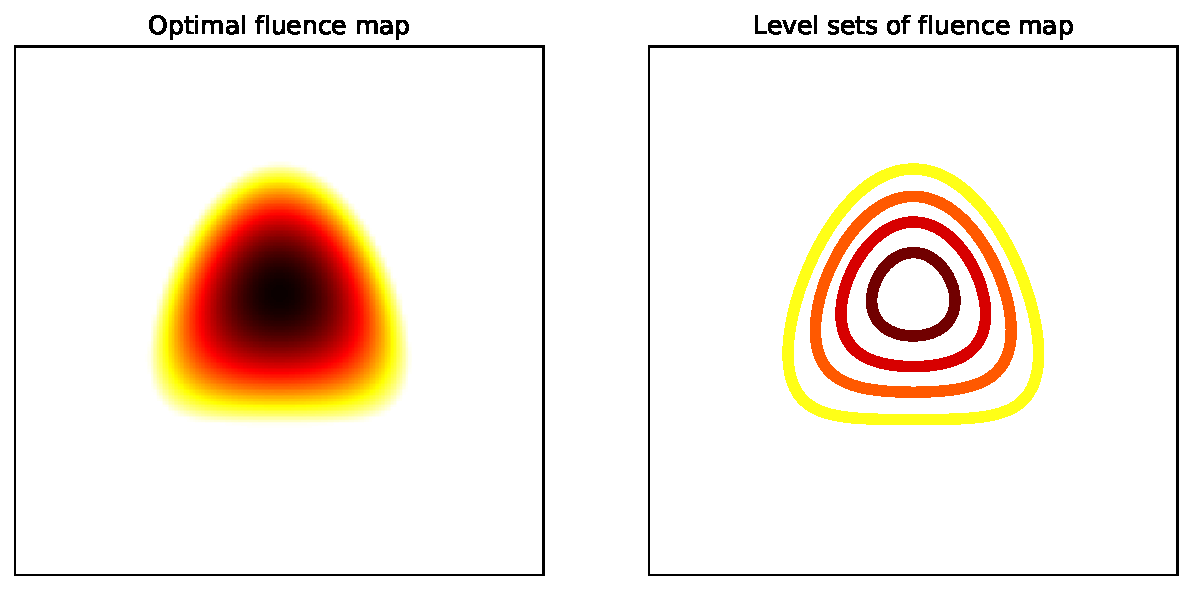
\includegraphics[height=4.5cm]{_fluence_map_discretization.pdf}
	\caption{Example of a fluence map discretization.}
	\label{fig:fluence_map_discretization}
\end{figure}
The fluence maps are divided into discrete levels (figure \ref{fig:fluence_map_discretization}).
\begin{figure}
	\centering
	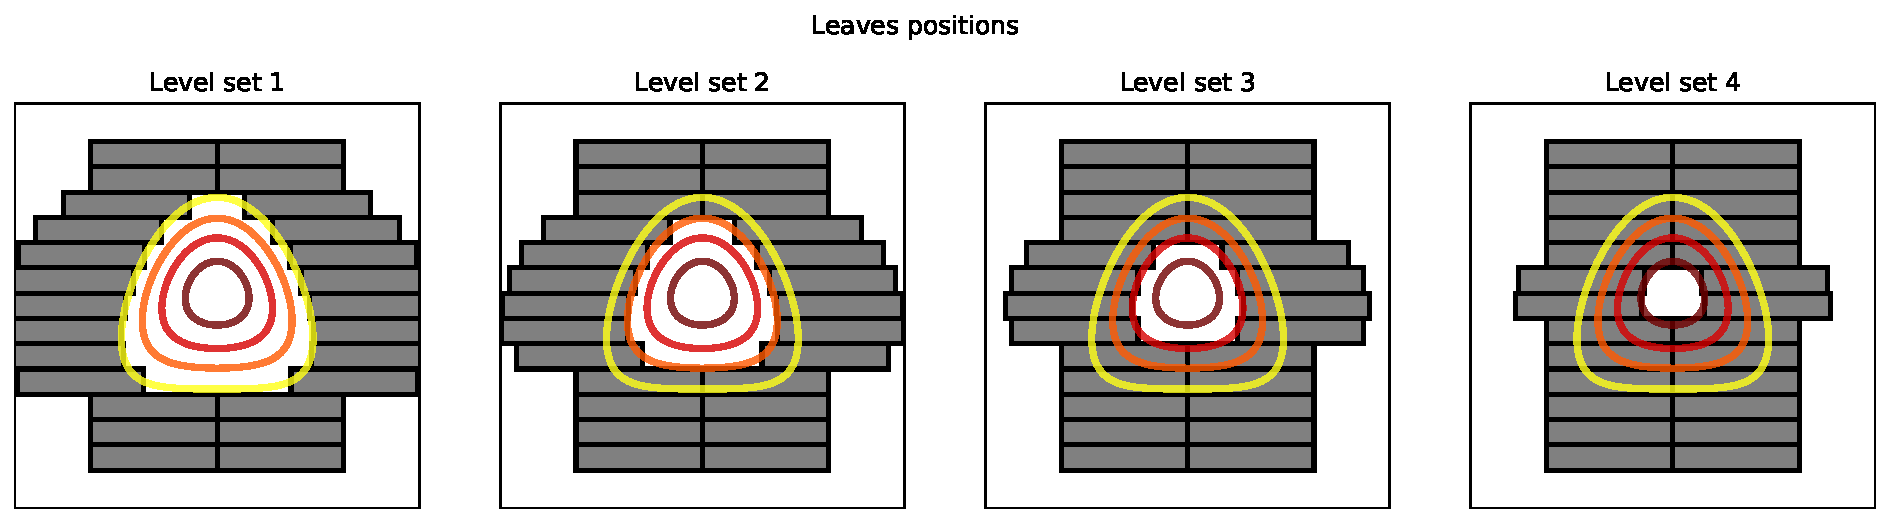
\includegraphics[height=4cm]{_level_set_matching_with_leaves.pdf}
	\caption{Example of level set matching with leaves.}
	\label{fig:level_set_matching_with_leaves}
\end{figure}
Then, the MLC leaves are positioned so that the open area of the irradiation head matches the level set (figure \ref{fig:level_set_matching_with_leaves}).
\begin{figure}
	\centering
	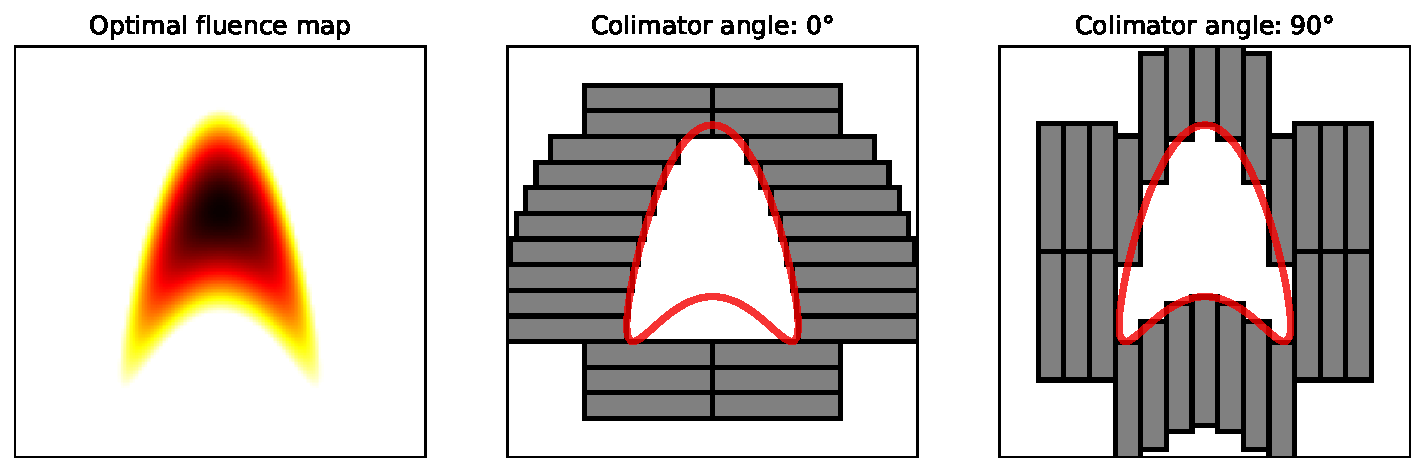
\includegraphics[height=4.2cm]{_leaves_angle.pdf}
	\caption{Example of a concave level matched with leaves.}
	\label{fig:leaves_angle}
\end{figure}
Note that convex level sets can all be matched with the MLC leaves; in case the level set is concave, changing the collimator angle may still allow the leaves to match the level set shape (figure \ref{fig:leaves_angle}).
Each level set is delivered as a static beam in sequence.
As the level sets are refined, the irradiation time increases
There is therefore a tradeoff to find between achieving greater accuracy and maintaining an efficient treatment time.

\paragraph[SW]{Sliding Window}
The "Sliding Window" technique, in contrast, is more computationally intensive:
The MLC leaves continuously move during beam delivery.
Finding the appropriate leaves motions requires solving a linear programming problem for each pair of leaves (sometimes called "Inverse Sliding Window Algorithm").
The fluence is segmented in one dimensional fluence curve along each leaf pair axis.
Correctly solving the linear programming problem allows a leaf pair to deliver any fluence within arbitrary approximation, in a reasonable amount of time.
A playground to calculate the leaves motion for an arbitrary fluence is available here:
\url{https://mics-lab.github.io/PresentationJuin2023PRFD/demo}.
% add playground demo for multi-leaf?

The sliding window technique is used most of the time, as delivery time is much (about twice) faster \cite{Ning2003}.

\subsection[DAO]{(Optional) Direct Aperture Optimization}
% mostly used for VMAT
% is sometimes used to fine tune IMRT



% %%%%%%%%%%%%%%%%%%%%%%%%%%%%%%%%%%%%%%%%%%%%%%%%%%%% %
% %%%%%%%%%%%%%%%%%%%%%%%%%%%%%%%%%%%%%%%%%%%%%%%%%%%% %
% %%%%%%%%%%%%%%%%%%%%%%%%%%%%%%%%%%%%%%%%%%%%%%%%%%%% %
% %%%%%%%%%%%%%%%%%%%%%%%%%%%%%%%%%%%%%%%%%%%%%%%%%%%% %
% %%%%%%%%%%%%%%%%%%%%%%%%%%%%%%%%%%%%%%%%%%%%%%%%%%%% %



\section{Simulation}
lots of approximations were made in the dosimetry, so there is a need to re-simulate to check that the machine instructions send a dose that is not too far from what was expected .
% https://oncologymedicalphysics.com/dose-calculation-algorithms/



% %%%%%%%%%%%%%%%%%%%%%%%%%%%%%%%%%%%%%%%%%%%%%%%%%%%% %
% %%%%%%%%%%%%%%%%%%%%%%%%%%%%%%%%%%%%%%%%%%%%%%%%%%%% %
% %%%%%%%%%%%%%%%%%%%%%%%%%%%%%%%%%%%%%%%%%%%%%%%%%%%% %
% %%%%%%%%%%%%%%%%%%%%%%%%%%%%%%%%%%%%%%%%%%%%%%%%%%%% %
% %%%%%%%%%%%%%%%%%%%%%%%%%%%%%%%%%%%%%%%%%%%%%%%%%%%% %



\section{Treatment Planning Systems}
Treatment Planning Systems (TPS) are the crucial tools that calculate the precise machine (MLC) motions according to the dosimetrists priorities and the irradiation technique chosen.

\subsection{Manufacturer}
%\columnratio{0.6}
%\begin{paracol}{2}
%	\paragraph{Eclipse\texttrademark\ (Varian)}
%	\ \\
%	Eclipse\texttrademark\ \cite{eclipse}, developed by Varian, is one of the most widely used TPS globally.
%	It supports VMAT with one or multiple arcs, and IMRT with any number of beams.
%	Eclipse\texttrademark\ integrates with Varian's suite of treatment machines, and integrates an automatic contouring tool \cite{eclipse_brochure}.
%	
%	\switchcolumn
%	
%	\begin{figure}[H]
%		\centering
%		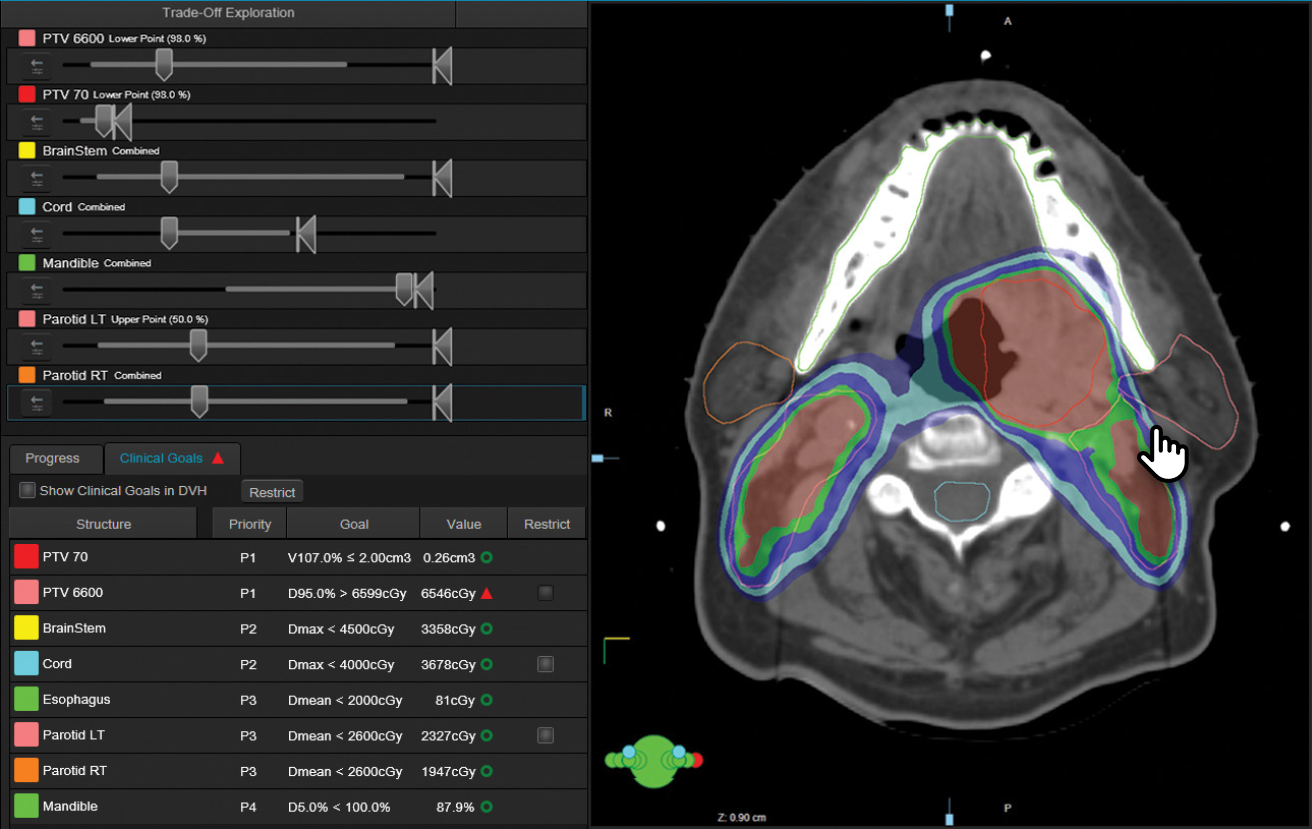
\includegraphics[width=\linewidth]{EclipseVarian.png}
%		\caption{Advertisement screenshot of \\ Eclipse\texttrademark\ (Varian's TPS).}
%		\label{fig:screenshot_eclipse}
%	\end{figure}
%\end{paracol}
\begin{multicols}{2}
	\paragraph{Eclipse\texttrademark\ (Varian)}
	\ \\
	Eclipse\texttrademark\ \cite{eclipse}, developed by Varian, is one of the most widely used TPS globally.
	It supports VMAT with one or multiple arcs, and IMRT with any number of beams.
	Eclipse\texttrademark\ integrates with Varian's suite of treatment machines, and integrates an automatic contouring tool \cite{eclipse_brochure}.
	
	\columnbreak
	
	\begin{figure}[H]
		\centering
		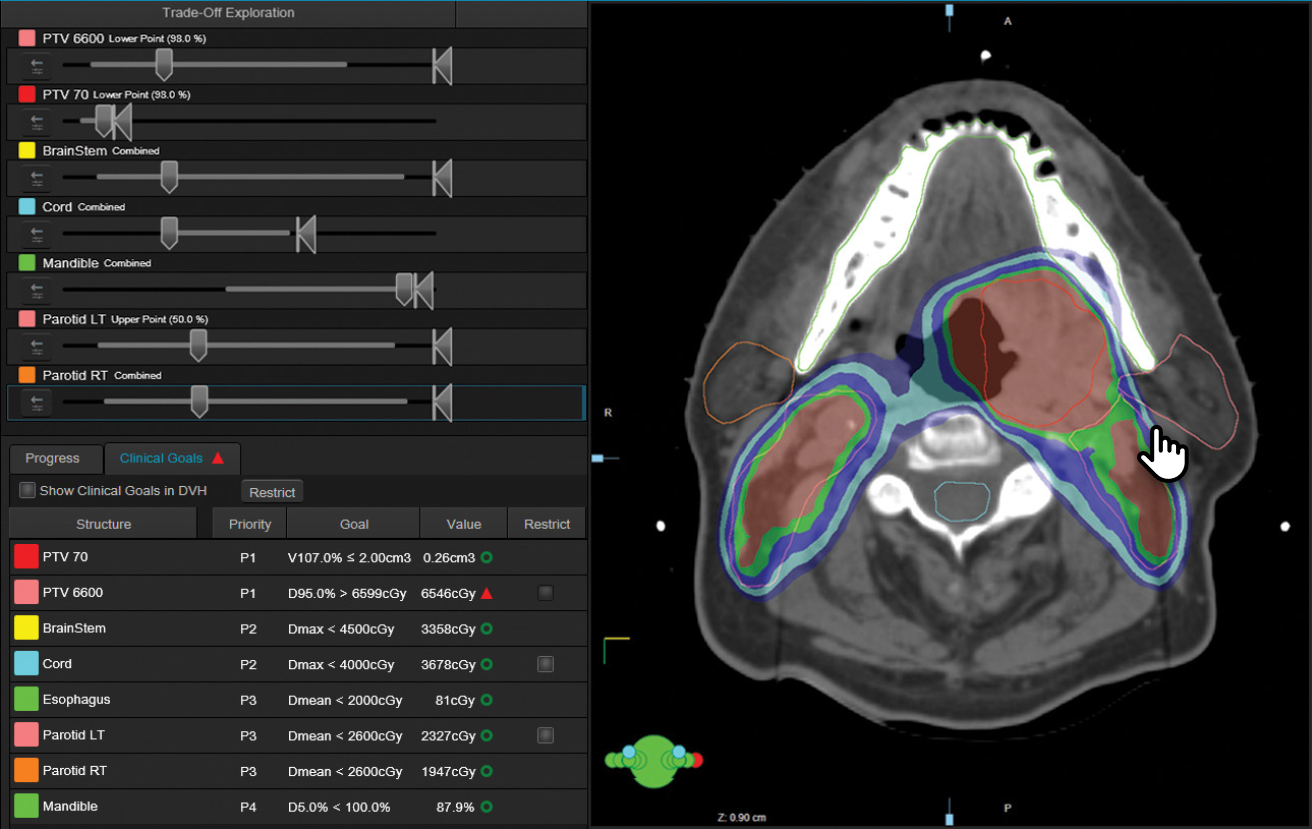
\includegraphics[width=\linewidth]{EclipseVarian.png}
		\caption{Advertisement screenshot of \\ Eclipse\texttrademark\ (Varian's TPS).}
		\label{fig:screenshot_eclipse}
	\end{figure}
\end{multicols}

\begin{multicols}{2}
	\paragraph{ONE® | Planning (Elekta)}
	\ \\
	ONE® | Planning \cite{one_planning} is Elekta's TPS, and is also widely used, supporting IMRT and VMAT.
	It is renowned for its speed with high-precision dose calculation using the Monte Carlo method.
	
	\columnbreak
	
	\begin{figure}[H]
		\centering
		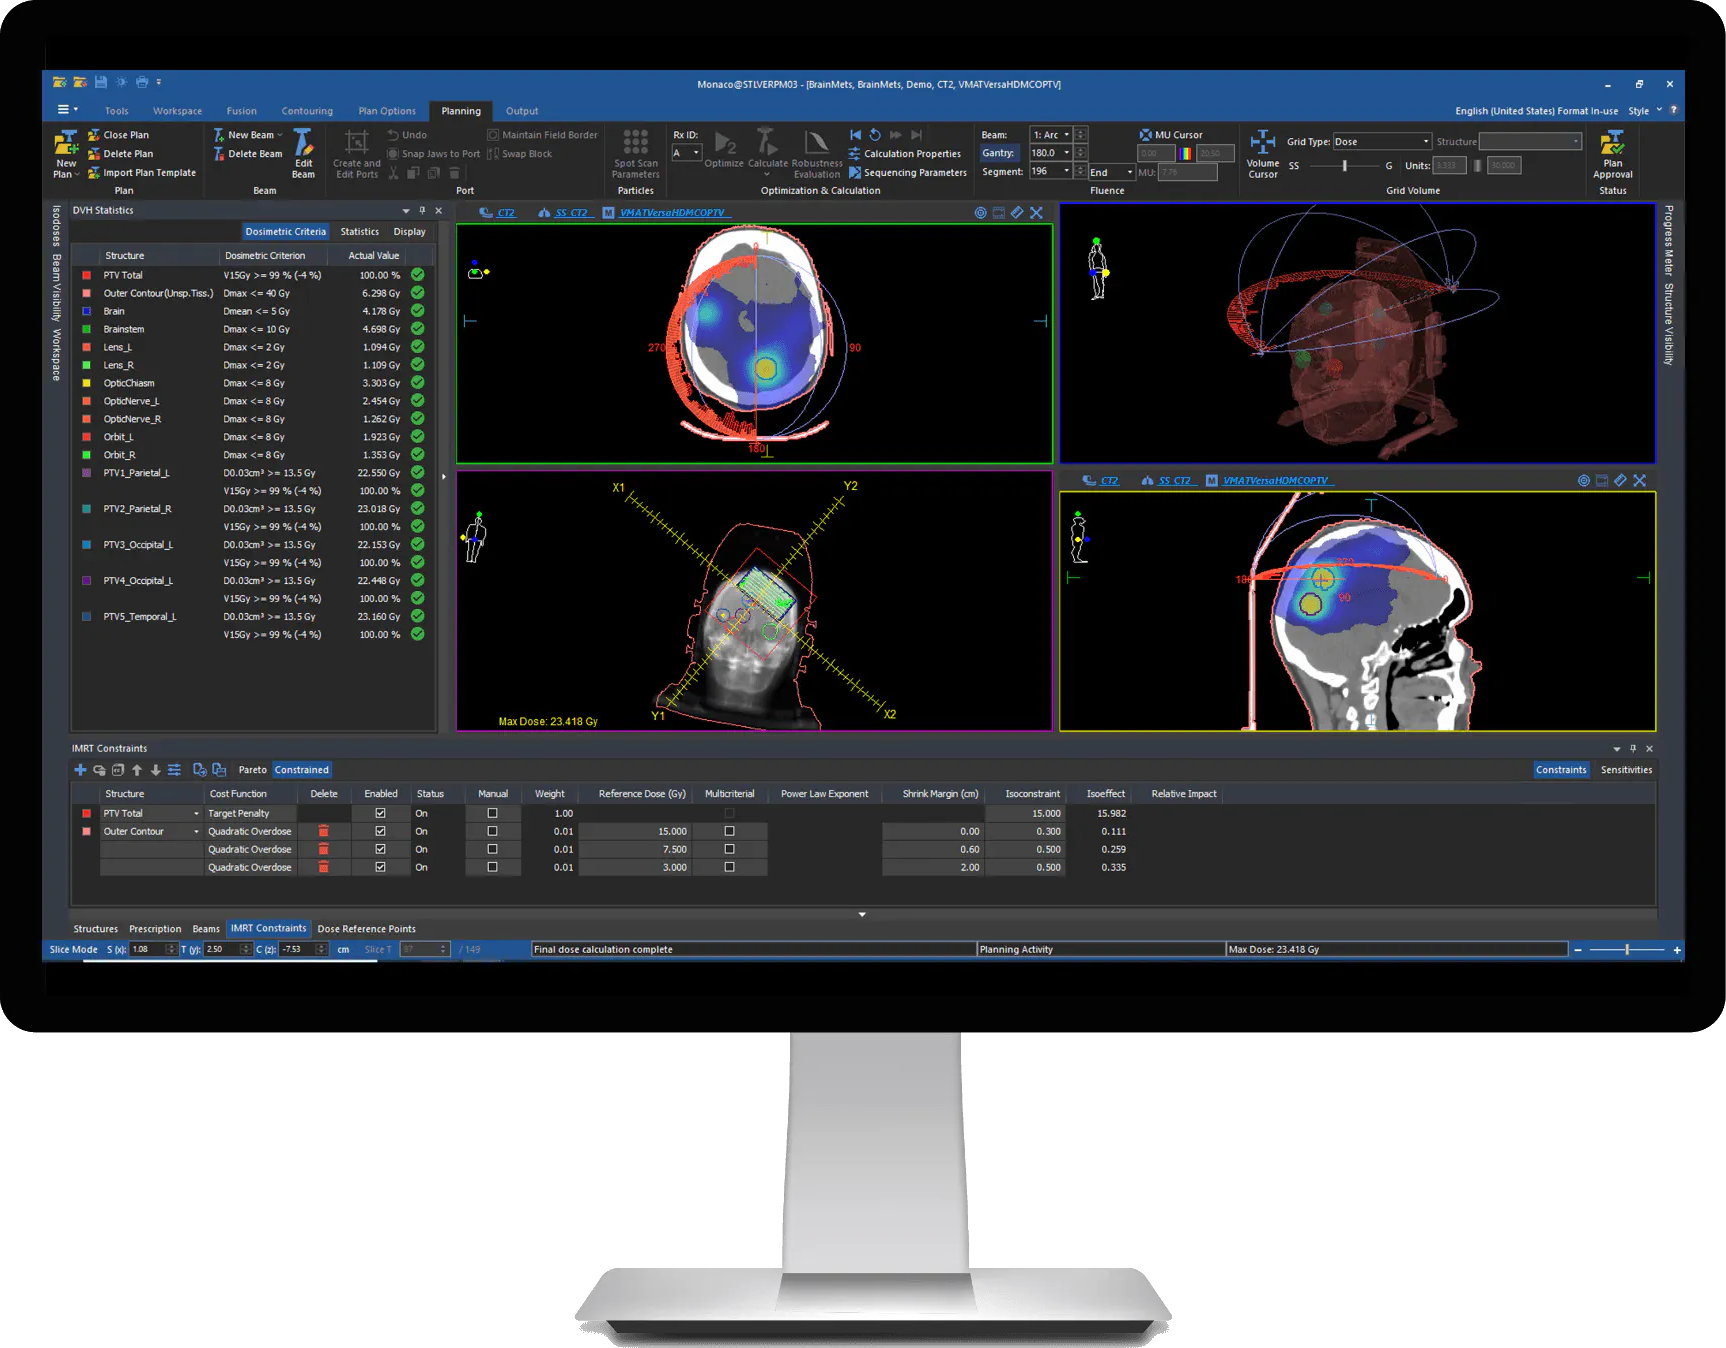
\includegraphics[width=\linewidth]{OnePlanningElekta.png}
		\caption{Advertisement screenshot of \\ ONE® | Planning (Elekta's TPS).}
		\label{fig:screenshot_one_planning}
	\end{figure}
\end{multicols}

\begin{multicols}{2}
	\paragraph{Precision® (Accuray)}
	\ \\
	Developed by Accuray, Precision® \cite{precision} is the dedicated TPS for CyberKnife and TomoTherapy systems.
	
	\columnbreak
	
	\begin{figure}[H]
		\centering
		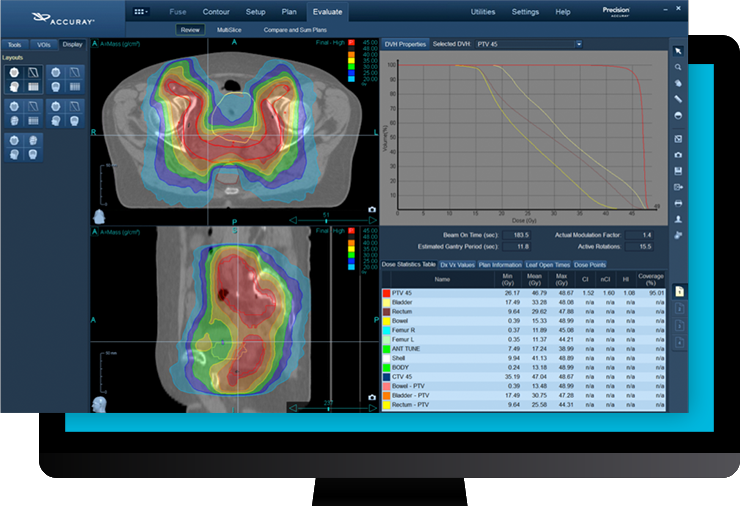
\includegraphics[width=\linewidth]{PrecisionAccuray.png}
		\caption{Advertisement screenshot of \\ Precision® (Accuray's TPS).}
		\label{fig:screenshot_precision}
	\end{figure}
\end{multicols}

\subsection{Non-manufacturer}
\begin{multicols}{2}
	\paragraph{RayStation (RaySearch)}
	\ \\
	RayStation \cite{raystation}, developed by RaySearch Laboratories, is a TPS known for its advanced optimization algorithms.
	Unlike manufacturer-specific systems, RayStation can output plans for a wide range of linear accelerators and imaging devices.
	It offers robust support for various treatment techniques, including VMAT, IMRT, 3D-CRT, Cyberknife, and TomoTherapy.
	
	\columnbreak
	
	\begin{figure}[H]
		\centering
		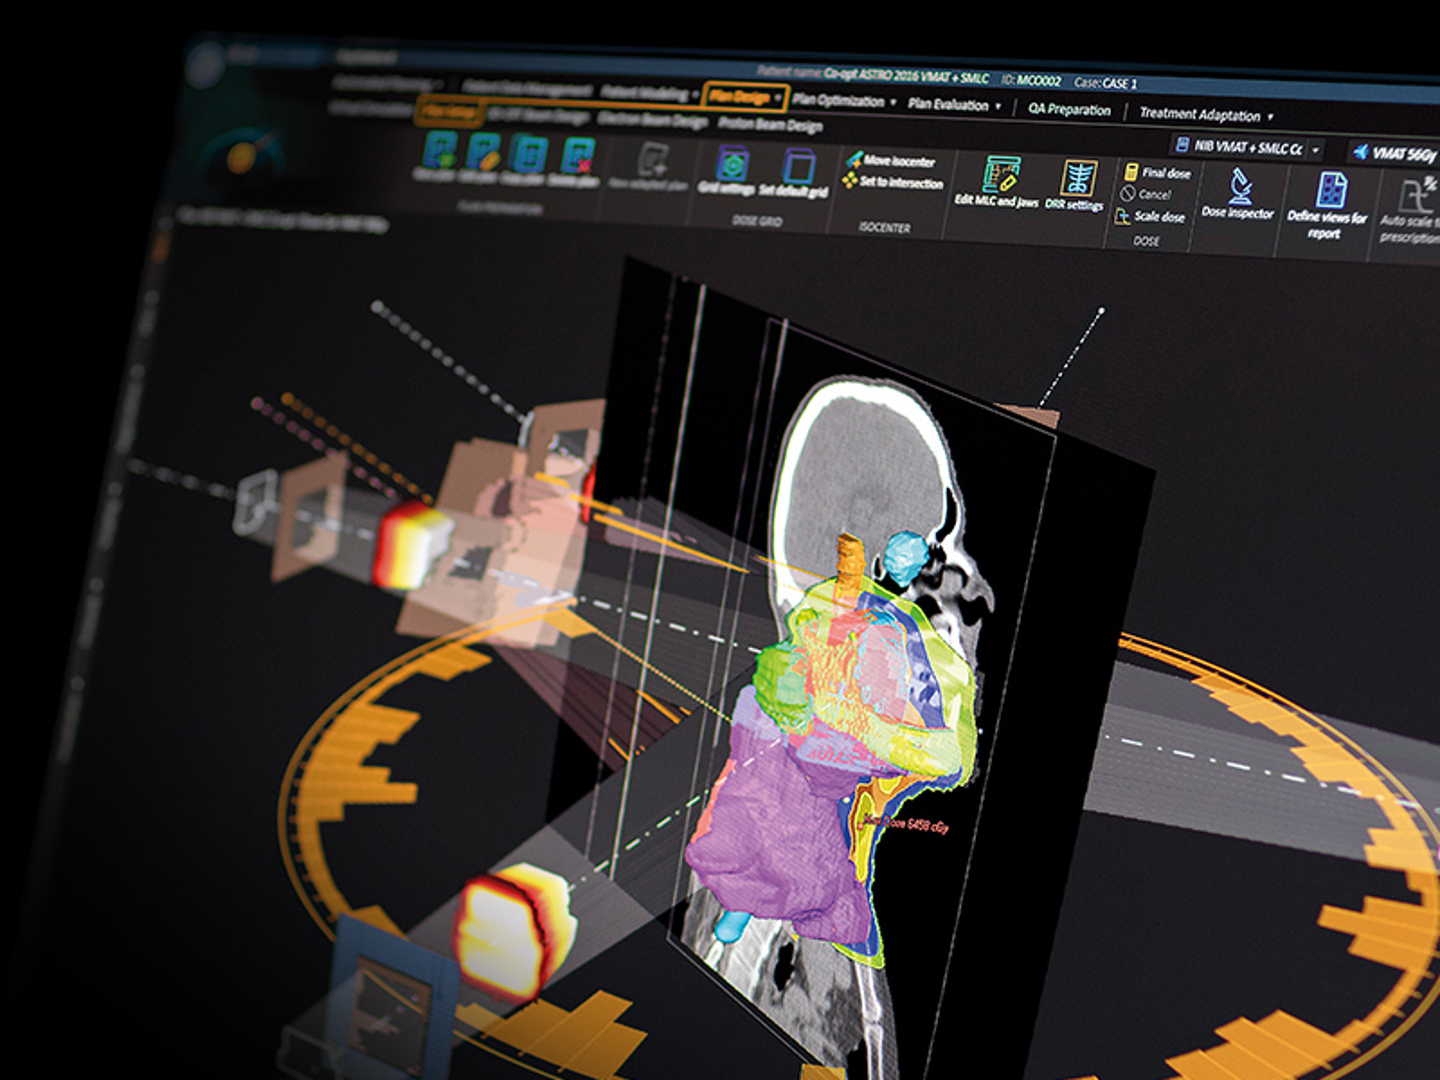
\includegraphics[width=\linewidth]{RaySearchRayStation.png}
		\caption{Advertisement screenshot of \\ RayStation (RaySearch's TPS).}
		\label{fig:screenshot_raysearch}
	\end{figure}
\end{multicols}

\begin{wrapfigure}{r}{0.3\textwidth}
	\vspace{-0.5cm}
	\centering
	
\includegraphics[width=0.3\textwidth]{matRad.png}
	\caption{matRad Logo}
	\label{fig:matRad_logo}
	\vspace{-0.5cm}
\end{wrapfigure}
\paragraph{matRad (German Cancer Research Center - DKFZ)}
\ \\
matRad \cite{matrad} is an open-source TPS developed by the German Cancer Research Center (DKFZ) for research and education.
While not intended for clinical use, matRad offers a flexible platform for testing and developing new treatment-planning algorithms.

\paragraph{AutoPlan (TheraPanacea - Unpublished)}
\ \\
AutoPlan is the upcoming TPS from TheraPanacea, designed to incorporate artificial intelligence and machine learning into the treatment planning process.


	
	\chapter{Introduction}
	\begin{chapterabstract}
		\lipsum[1-2]
	\end{chapterabstract}
	\clearpage
	\localtableofcontents
	\section{Context}
Cancer remains one of the leading causes of mortality worldwide, with its incidence projected to rise in the coming decades \cite{Quante2016,Smittenaar2016}.
As our understanding of cancer biology evolves and diagnostic techniques improve, the demand for effective and personalized treatment strategies continues to grow \cite{Howard2017}.
Radiotherapy has emerged as a cornerstone in cancer management, either as a standalone treatment or in combination with other modalities such as surgery, chemotherapy, and immunotherapy \cite{Rivoirard2015,Reynders2015}.
Radiotherapy leverages ionizing radiation to damage cancer cells' DNA, impeding their ability to proliferate and ultimately leading to cell death \cite{Yard2015}.
The efficacy of radiotherapy lies in its ability to deliver precise doses of radiation to tumor volumes while minimizing exposure to surrounding healthy tissues \cite{Malicki2012}.
This delicate balance between tumor control and normal tissue toxicity underscores the importance of treatment planning in radiotherapy \cite{Das2009}.

The advent of advanced imaging technologies \cite{Li_Zhang_2024}, coupled with sophisticated delivery systems like Multi-Leaf Collimator Linear Accelerators (MLC-LINACs), Tomotherapy units, and CyberKnife systems, has revolutionized the field of radiation oncology \cite{Klein_2009,Xia2001}.
These technological advancements have paved the way for highly conformal treatment techniques.
Intensity-Modulated Radiation Therapy (IMRT) and Volumetric Modulated Arc Therapy (VMAT) techniques offer unprecedented levels of dose sculpting, allowing for escalated doses to tumors while better sparing organs at risk \cite{Ng2018,Elith2011,Davidson2011}.
However, the increased complexity of modern radiotherapy techniques has led to a corresponding increase in the complexity of treatment planning \cite{Fraass2012,Robinson2008}.
The process of creating an optimal treatment plan involves multiple steps, including Beam Orientation Optimization (BOO) \cite{Pugachev2000,Pugachev2001}, Fluence Map Optimization (FMO) \cite{Lim2008,Romeijn_2004,Lee2006}, Leaf Sequencing (LS) \cite{Chen2003,Chen2005,Xia2002}, and (sometimes) Direct Aperture Optimization (DAO) \cite{Shepard2002,Earl_2003,Ahunbay2007}.
Each step requires careful consideration of numerous variables and constraints, making the planning process time-consuming and labor-intensive \cite{Wang2019}.

In this context, this thesis aims to explore and advance the radiotherapy treatment planning automation field, focusing on developing novel algorithms and methodologies to enhance treatment plans' efficiency, quality, and consistency.
By building upon the foundational knowledge of radiotherapy physics, biology, and clinical workflow, we seek to contribute to the ongoing evolution of radiation oncology and, ultimately, to improve outcomes for cancer patients.

\section{Problematic}
Traditional manual radiotherapy planning procedures are inherently subjective and time-consuming.
The reliance on individual planner expertise often leads to variability in treatment plan quality\cite{Chung2008,Bohsung2005,Das2008,Williams2007}.
This treatment plan diversity can induce inconsistencies in patient care.
While efforts have been made to enhance consistency \cite{Bahm2011}, significant variability among planners and institutions persists.
There is a pressing need for more standardized planning approaches.
The automation of treatment planning processes presents a promising solution to these challenges.

Moreover, the time-intensive nature of manual optimization \cite{Zhang2020} and the growing demand for radiotherapy services have created a pressing need to develop automated approaches to streamline the radiotherapy planning process.
Automation enables the treatment of more patients and facilitates exploring a broader range of treatment options.

By applying computational algorithms and artificial intelligence, automated planning systems offer the potential to enhance radiotherapy treatment delivery significantly.
These systems can improve patient throughput and resource allocation by reducing planning time and increasing departmental efficiency.
Automated planning can improve plan quality and consistency, reducing variability and ensuring optimal treatment outcomes.
Furthermore, the ability to enable rapid re-planning facilitates adaptive radiotherapy, allowing for adjustments to treatment plans in response to changes in tumor volume or patient anatomy.
Finally, automated systems can explore a more expansive solution space, potentially discovering novel and innovative planning strategies that may improve treatment outcomes.

However, the development and implementation of automated planning systems pose challenges.
These challenges include the creation of robust optimization algorithms, integrating with existing Treatment Planning Systems, and validating against current clinical standards.

\section{State of the Art}
\paragraph{Knowledge-based radiotherapy planning}
Knowledge-based radiotherapy planning (KBRP) represents an objective methodology for incorporating patient-specific data and historical experience into the treatment planning process \cite{Nwankwo_2014}.
By automating the optimization of KBRP, it is anticipated that a viable alternative to the current human-centric treatment planning paradigm can be established.
A prevalent KBRP approach involves leveraging a database of historical benchmark plans to learn patient-specific dosimetric parameters and generate new treatment plans.
Automated KBRP tools effectively set optimization parameters based on the desired dose-volume histogram.
Previous studies have reported notable dosimetric improvements in treatment plans generated by KBRP approaches compared to benchmark data, particularly regarding sparing organs at risk \cite{Fogliata2014,Tol2015}.

\paragraph{Conventional techniques}

\paragraph{Pareto surface exploration}
In DVH-based inverse optimization used by most commercial TPS, a cost function must be defined to solve the minimization problem.
This function combines data from all volumes of interest as a weighted sum of penalties from each DVH constraint.
The weighting coefficients reflect trade-offs between the target(s) and different OARs.
However, this approach requires reoptimization if dosimetric preferences change during plan evaluation, making it time-consuming to find the optimal balance.
To address this, multi-criteria optimization (MCO) was introduced, enabling the simultaneous generation of multiple "anchor" plans.
Each anchor plan optimizes one OAR’s DVH criterion for maximal sparing without compromising tumor target dosimetry.
These plans form a hypersurface in the $N$-dimension space, where $N$ is the number of independent OAR dosimetric constraints.
Referred to as the Pareto surface, this hypersurface contains the optimal plans following different dosimetric criteria.

Previous research has explored Pareto optimal tradeoffs in various domains.
Gebru et al., for instance, investigated methods for evaluating Pareto optimality \cite{Gebru2023}.
Similarly, Cilla et al. conducted a comprehensive analysis of Pareto fronts \cite{Cilla2018}.
These studies provide valuable insights into the principles and techniques associated with Pareto optimization.
Craft et al. proposed a method for generating multiple Pareto optimal dose distributions, allowing clinicians to make informed decisions based on their specific preferences and clinical contexts \cite{Craft2007}

\section{Unsolved problems}
Numerous approaches have been investigated to automate the radiotherapy treatment planning process.
Despite these efforts, a consensus on the optimal method has yet to be established, and few automated solutions have been adopted in clinics.
The challenges associated with automating radiotherapy treatment planning remain a significant area of inquiry within the field.
This thesis addresses this critical issue by proposing advancements in key areas that may contribute to developing a fully automated treatment planning system.

\section{Thesis overview}
This section provides a comprehensive summary of the forthcoming chapters of this thesis.

\subsection{Fluence Map Optimization}
Chapter 3 is dedicated to developing computational methods for Fluence Map Optimization (FMO).
The chapter begins by assessing the discretization strategies.
Naive approaches for optimization are explored, stepping up to a formalization of the classical FMO problem.
A significant focus is placed on incorporating medical constraints and the corresponding importance factors associated with each constraint, which are critical in ensuring clinically viable treatment plans.
The performance of various optimization algorithms is evaluated and compared, providing insights into their relative efficiencies in solving the FMO problem.
This primary work was published in the form of an ArXiV article.

\subsection{Semi-automation}
\subsubsection*{Using graph-based analysis}
Chapter 4 explores the interrelationships between radiotherapy treatment plans by defining a distance metric.
This distance is then used to cluster plans into meaningful groups.
The clustering forms a basis for developing a semi-automated framework for treatment plan optimization.
Leveraging graph-based methodologies, this approach reduces the need for manual intervention in the planning process while ensuring the generation of high-quality plans.
The potential of this semi-automated framework to streamline clinical workflows was presented at the 2024 European Society for Radiotherapy and Oncology (ESTRO) conference.

\subsection{Full-automation}
\subsubsection*{With reinforcement learning and conventional treatment optimization techniques}
Chapter 5 addresses the limitations of classical optimization techniques in fully automating the treatment planning process.
This chapter introduces a novel framework that integrates reinforcement learning with conventional optimization.
The reinforcement learning agent is driven by clinical expertise and can be specialized to center-specific guidelines.
The findings from this work have been disseminated through a peer-reviewed journal article, a presentation at the Artificial Intelligence in Medicine (AIME) 2024 conference, and a poster presentation at the American Society for Radiation Oncology (ASTRO) 2024 meeting.

\subsection{Hybrid-automation}
\subsubsection*{Via target DVHs deep dose and dose mimicking technique}
The final research chapter, Chapter 6, presents a hybrid approach to automating treatment planning.
This approach combines deep learning for dose prediction with target Dose-Volume Histograms (DVHs) and plan-mimicking strategies.
This methodology bridges the gap between fully automated AI-driven techniques and traditional planning methods, offering a more adaptable and clinically feasible solution.
The hybrid model provides a mechanism for mimicking high-quality plans from experienced planners.
This research has been presented at the French Society of Medical Physics (SFPM) and the French Society for Radiation Oncology (SFRO) 2024 meetings.

	
	\chapter{Dosimetry Optimization}
	\begin{chapterabstract}
		Biological tissues are sensible to radiations in a non-linear manner \cite{Liu2003}, and slight variations in dose can have significant biological effects.
Organs have differing sensibilities to radiation, which increases further the difficulty in formulating the goals to achieve when designing a radiation dose.
Some organs can tolerate high cumulative doses if the radiation is well distributed.
In contrast, others may withstand high doses at localized points ("hot spots") but cannot handle large doses overall.
To address these differences, clinicians impose dose-volume histogram constraints in addition to the prescribed dose.
Although the ideal objective is to minimize or eliminate radiation exposure to organs, achieving $0\,\text{Gy}$ is impossible.
The necessity of finding compromises drives the need for advanced optimization techniques to generate fluence maps that best satisfy the medical constraints.
Therefore, various techniques can be used to calculate fluence maps (i.e., performing the critical fluence map optimization step).
In this chapter, we explore some fluence map optimization techniques.
% These techniques will be used in the remaining manuscript.

	\end{chapterabstract}
	\clearpage
	\localtableofcontents
	%In modern radiotherapy, the precision of dose delivery is essential to maximize the therapeutic effect on cancerous tissues while minimizing exposure to surrounding healthy organs.
%Achieving this balance relies heavily on advanced dose optimization techniques that tailor radiation to each patient's specific anatomical and clinical needs.
\section{Discretization}
The optimization process starts with transforming the continuous nature of both the radiation field and the human body into discrete elements.
This transformation enables computation with modern computers.

\subsection[Bixels]{Fluence Map Discretization: Bixels}
Fluence maps are broken down into discrete elements called "bixels" (\textbf{be}am \textbf{el}ements).
Bixels represent small and independent beams of radiation.

The width of each bixel is constrained by the width of the multi-leaf collimator leaves.
Modern multi-leaf collimator systems typically have a leaf width of 0.5 cm.

The height of a bixel can be selected arbitrarily, as the leaf can move continuously.
Nevertheless, square bixels (akin to image pixels) are commonly used and will be employed throughout this manuscript.

Bixels whose beams do not affect the planning target volume are typically excluded from calculations to improve computational efficiency.
Activating these bixels could only degrade dose quality by increasing the dose to organs at risk without benefiting the dose distribution within the planning target volume.

\subsection[Voxels]{Human Body Discretization: Voxels}
The human body of the patient is also divided into discrete elements, as it is a three-dimensional object; the elements are "voxels" (\textbf{vo}lume \textbf{el}ements).
Each voxel represents a small portion of tissue within the patient's body, and will determine the granularity of the dose computed.

The maximum resolution of the voxel grid is defined by the planning image, which is typically a CT scan.
It is common practice to resample the planning image to reduce computational demands.
In this manuscript, where new techniques are explored, we have opted to resample the voxel grid to a resolution of 5 mm, ensuring a balance between computational efficiency and accuracy.

Additionally, to further optimize the computational process, only voxels corresponding to the planning target volume (PTV) and organs at risk (OARs) are retained for calculations.
This selective approach reduces unnecessary computation.

\subsection[DI-Matrix]{Dose-Influence Matrix}
The Dose-Influence Matrix (or DI-Matrix) links the discretized fluence map (the bixels values) and the discretized dose distribution within the patient (the dose on each voxel).
This matrix defines how the radiation from each individual bixel influences the dose delivered to every voxel in the patient's body.

We start by converting the 2D fluence map, composed of individual bixel values, into a column vector $b$.
Similarly, we represent dose distribution in the patient's 3D space as a vector $\mathbf{d}$, where each entry corresponds to the dose in a specific voxel.
The DI-Matrix $L$ governs the relationship between these vectors $\mathbf{b}$ and $\mathbf{d}$ via the matrix-vector multiplication $\mathbf{d} = L\mathbf{b}$.
This mathematical operation computes the total dose at each voxel by summing the contributions from all active bixels (here, we assume that the effect of bixels is linear).

The DI-Matrix is constructed by simulating the radiation delivered by each individual bixel.
For each bixel, the jaws of the multi-leaf collimator are virtually opened to allow only that specific beamlet to go through.
A radiation transport model calculates the dose deposited in each voxel, considering the beam's spread and attenuation as it travels through the body.
The resulting 3D dose deposition fills one column of the matrix $L$, corresponding to that bixel's influence on all voxels.
Repeating this process for each bixel generates the entire DI-Matrix.

The accuracy of the dose calculation depends on the precision of the DI-Matrix.
Simple models like pencil beam approximations, which assume a linear trajectory with minimal scattering, are considered too coarse.
In contrast, more advanced simulations, such as Monte Carlo methods, provide a detailed and accurate dose calculation, although at a higher computational cost.
In this manuscript, we employ collapsed cone convolution techniques, which balance efficiency and accuracy.

\section{Naive Optimization Method}
A natural starting point in dose optimization is to attempt to directly achieve the delivery of a uniform dose, equal to the prescription, on all voxels within the PTV, and no dose elsewhere.
We can attempt to find the bixels values delivering this dose by solving a least squares problem.
We attempt to find the fluence map $\mathbf{b}$ that minimizes the difference between the actual dose $\mathbf{d}$ and the target dose $\mathbf{d}_{\text{target}}$, which is set to the prescribed dose within the PTV.

Formally, the optimization problem can be stated as:
$$ \min_\mathbf{b} \| \mathbf{d}_{\text{target}} - L\mathbf{b} \|^2 $$

where $\mathbf{d}_{\text{target}}$ is the target dose vector, defined as follow for a prescription of $p$Gy:
$$ \mathbf{d}_{\text{target}} = p \cdot  \mathds{1}_{\text{PTV}} $$

Here, $\mathds{1}_{\text{PTV}}$ is the indicator vector for PTV that is equal to $1$ for voxels within the PTV and $0$ elsewhere.

To solve this problem, we perform a least squares minimization to find the optimal fluence map $\mathbf{b}$, where the matrix-vector multiplication $L\mathbf{b}$ yields the dose distribution $\mathbf{d}$ across the entire patient volume.

However, this method is often inadequate in practice, as it attempts to solve the system based solely on the prescribed dose within the PTV, while neglecting any constraints on doses to the organs at risk (OARs).
Since no constraints are imposed on the OAR doses, this naive optimization can result in high doses to critical structures, leading to unacceptable treatment plans.
As a result, more sophisticated optimization methods that incorporate dose constraints on OARs and account for dose-volume constraints are necessary to achieve clinically viable treatment plans.
% add 3D dose & DVHs of dose obtained using this technique

\section{Constraints and Importance Factors}
In order to obtain clinically acceptable doses, we need to incorporate the clinical aims in the optimization.

\subsection{Constraints Formulation}
Different organs exhibit varying sensitivities to radiation, which influence their dose tolerance limits \cite{Withers1988} \cite{ICRU83}.
Normal tissues are categorized as serial, parallel, or mixed, based on the functional organization of their sub-units.
This classification determines the appropriate absorbed dose limits for normal tissues.

Serial organs (figure \ref{fig:serial_organ}), such as the spinal cord or esophagus, are characterized by a functional dependence on the integrity of every sub-unit.
Damage to even a tiny region in these tissues can result in the loss of the organ's overall function.
In contrast, parallel organs (figure \ref{fig:parallel_organ}), such as the lung or liver, possess a reserve capacity where damage to a portion of the tissue does not necessarily impair overall function, as long as a critical volume remains intact.

\begin{figure}
	\begin{subfigure}{0.6\textwidth}
		\centering
		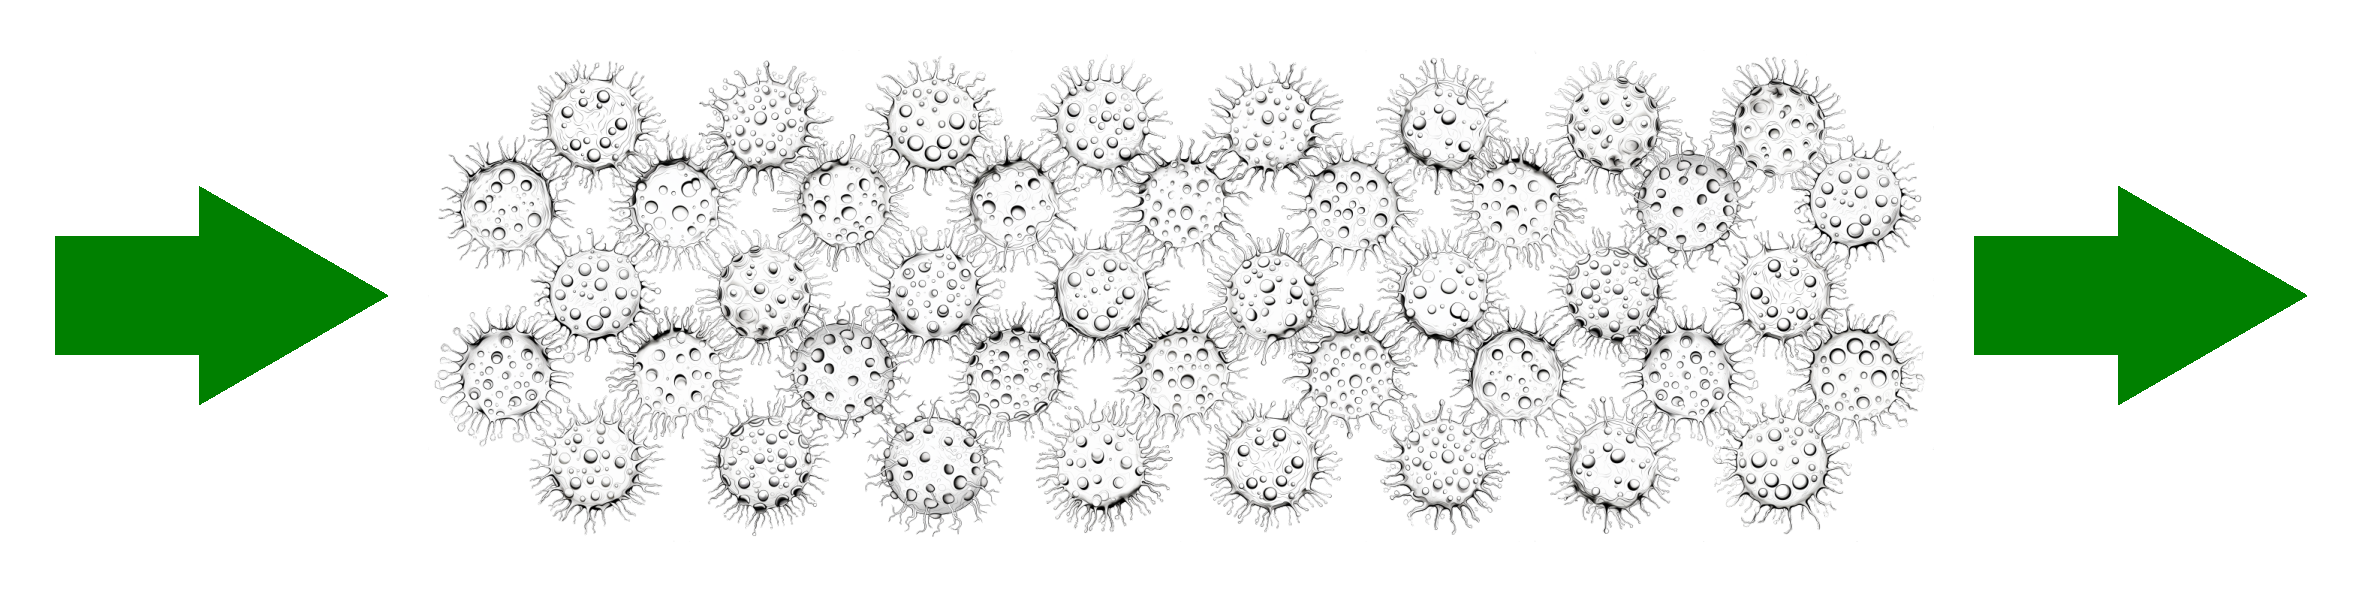
\includegraphics[width=0.9\textwidth]{serial_organ.pdf}
		\vspace{4mm}
		\caption{Organ functioning in a serial-like way.}
		\label{fig:serial_organ}
	\end{subfigure}
	\hfill
	\unskip\ \vrule\
	\hfill
	\begin{subfigure}{0.38\textwidth}
		\centering
		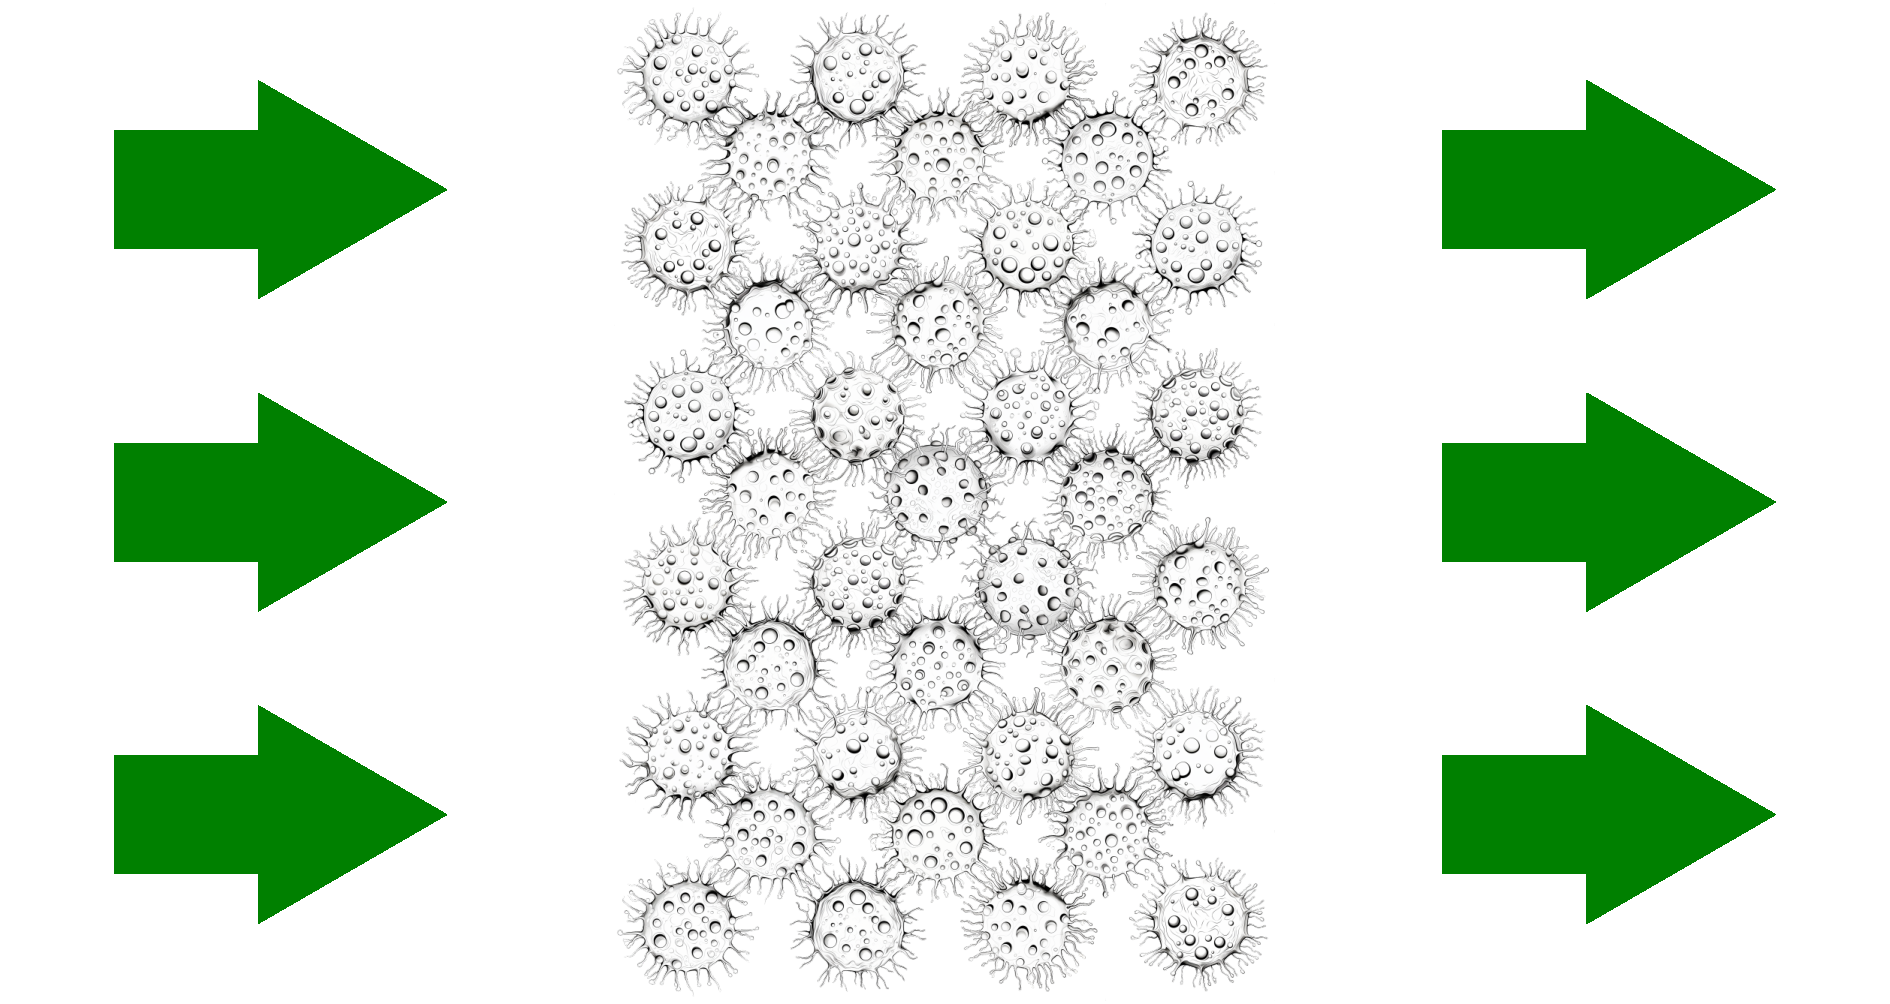
\includegraphics[width=0.9\textwidth]{parallel_organ.pdf}
		\caption{Organ functioning in a parallel-like way.}
		\label{fig:parallel_organ}
	\end{subfigure}
	\caption{Organs functioning types.}
	\label{fig:serial_parallel_organ}	
\end{figure}

We define two DVH value measures $V_X$ and $D_{X\%}$ for a structure $S$.
For a given dose $d: \R^3 \to \R^+$, $V_X$ is defined as the volume of the three dimensional structure $S \subseteq \R^3$ that receives a dose equal to or higher than $X$, that is:
$$ V_X = \frac{\vol{\left\lbrace p \in S \subset \R^3 \mid d(p) \geq X \right\rbrace}}{\vol{S}}.$$
This can be approximated using the discretized dose $\mathbf{d}$:
$$ V_X \approx \frac{ \#{\left\lbrace v \in S \mid \mathbf{d}_v \geq X \right\rbrace}}{\#\left\{ v \in S \right\}}$$
with $v \in S$ voxels of the structure $S$, $\mathbf{d}_v$ the dose of $\mathbf{d}$ associated with voxel $v$, and $\#$ refers to voxel count.

Similarly, we define $D_{X\%}$ as the minimal dose (in Gy) delivered to that the $X\%$ most irradiated region of the structure, that is:
$$D_{X\%} = \min \left\lbrace d(p) \mid p \in S_{X\%} \right\rbrace$$
where $S_{X\%} \subseteq S$ is the $X\%$ most irradiated region of $S$.
$$D_{X\%} \approx \min \left\lbrace \mathbf{d}_v \mid v \in S_{X\%} \right\rbrace$$
where $v \in S_{X\%}$ are the $X\%$ most irradiated voxels of $S$.

This $D_{X\%}$ can also be defined as the maximal dose $D$ such that $V_D$ the volume of $S$ that receives a dose equal to or higher than $D$ is greater than or equal to $X$:
$$D_{X\%} = \max \left\lbrace D \in \R^+ \mid V_D \geq X\% \right\rbrace.$$
The DVH curve is the plot of $x \mapsto V_x$ on the range of $d$.

For parallel-like structures, dose–volume reporting specifying $V_D$ is commonly used, with $D$ adapted to the specific organ.
For instance, \cite{Graham1995} demonstrated a correlation between the incidence and severity of lung pneumonitis and $V_{20 \text{ Gy}}$, the volume of the lung receiving more than 20 Gy.
Additionally, in parallel-like structures, the median absorbed dose ($D_{50\%}$), provides a valuable measure of the total dose delivered to the organ at risk.

For serial-like organs, it is recommended to report $D_{2\%}$ as the maximum absorbed dose, as $D_{0\%}$ is subject to noise.

Finally, for organs with a mixed parallel-serial structure, it is advised to report $D_{50\%}$, $D_{2\%}$, and $V_D$, with $D$ selected based on the threshold beyond which there is a significant risk of serious complications.

\begin{figure}
	\begin{subfigure}[b]{0.48\textwidth}
		\caption{Irradiation of organs at risk with one heat point.}
		\label{fig:organ_radiation_point}
		\centering
		\vspace{3mm}
		\hspace{1.2cm}
		Treatment Dose
		\\
		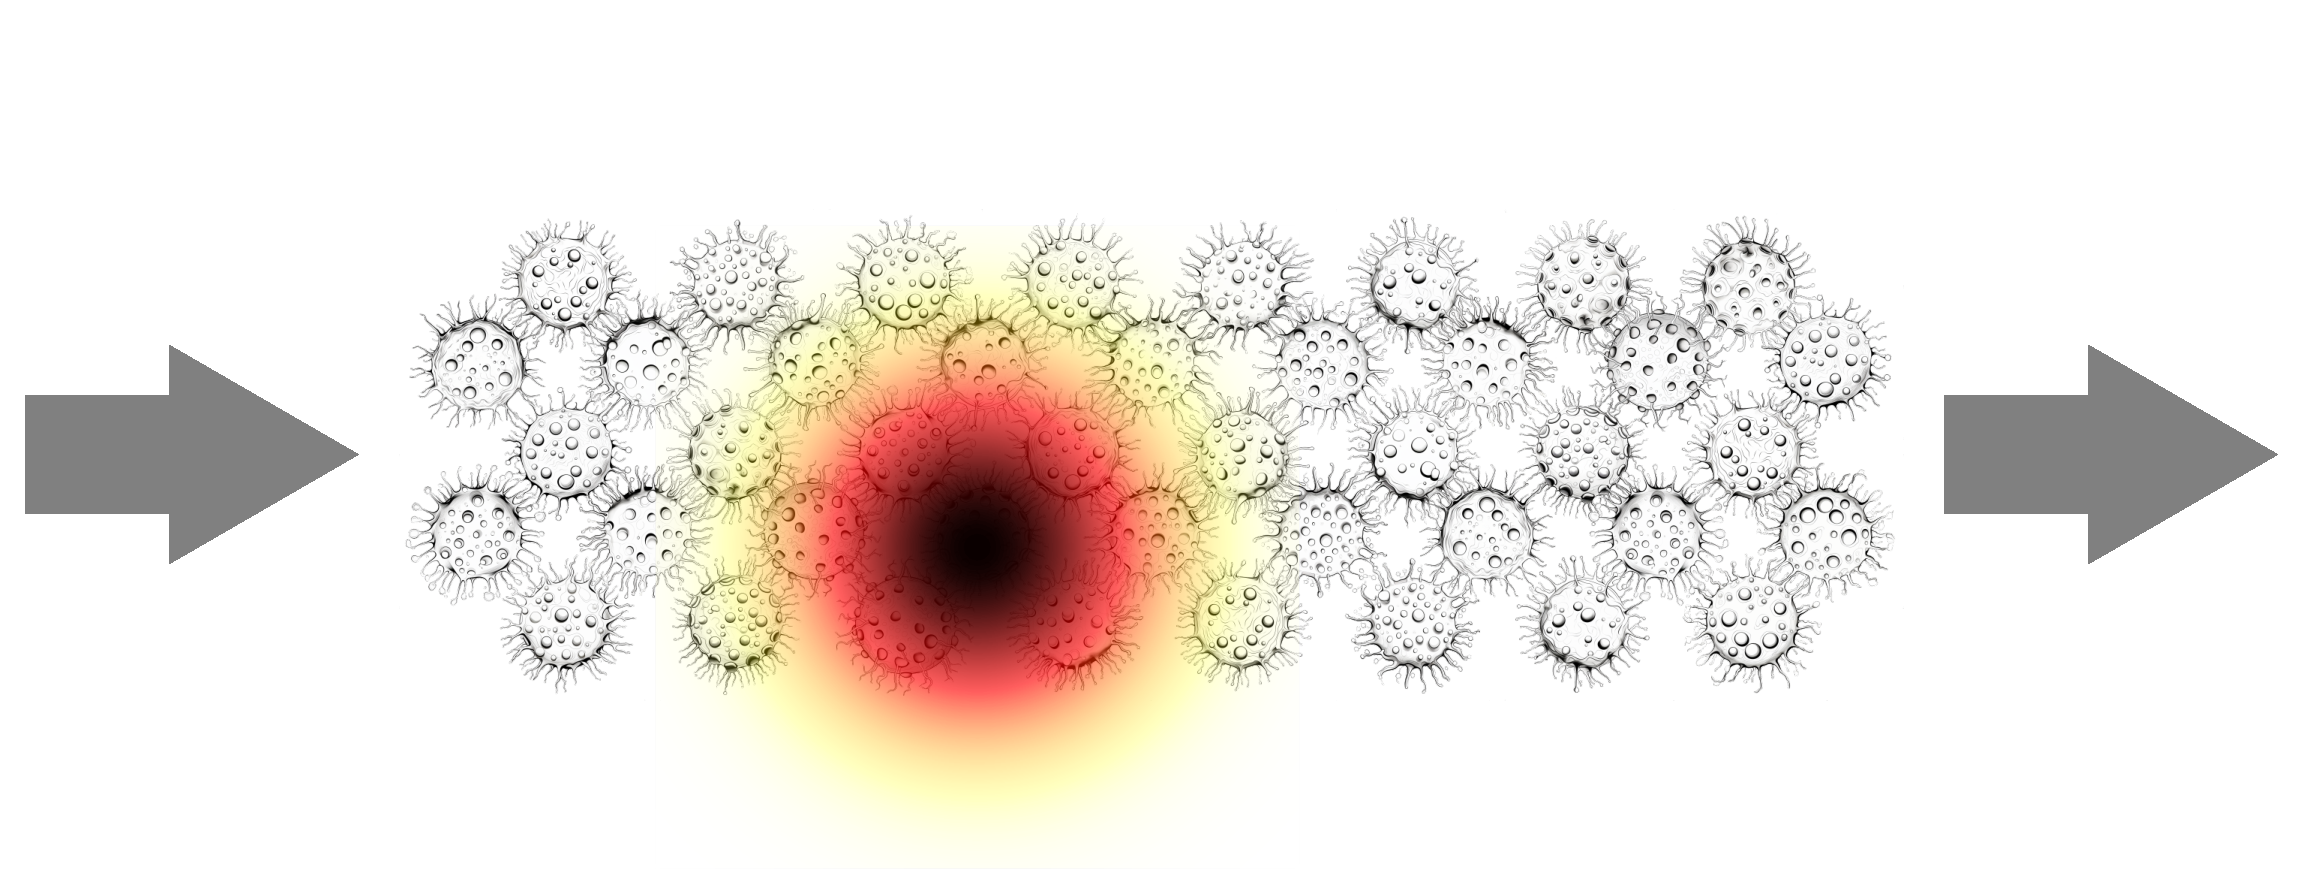
\includegraphics[width=0.55\textwidth]{serial_heat_point.pdf}
		\vbar
		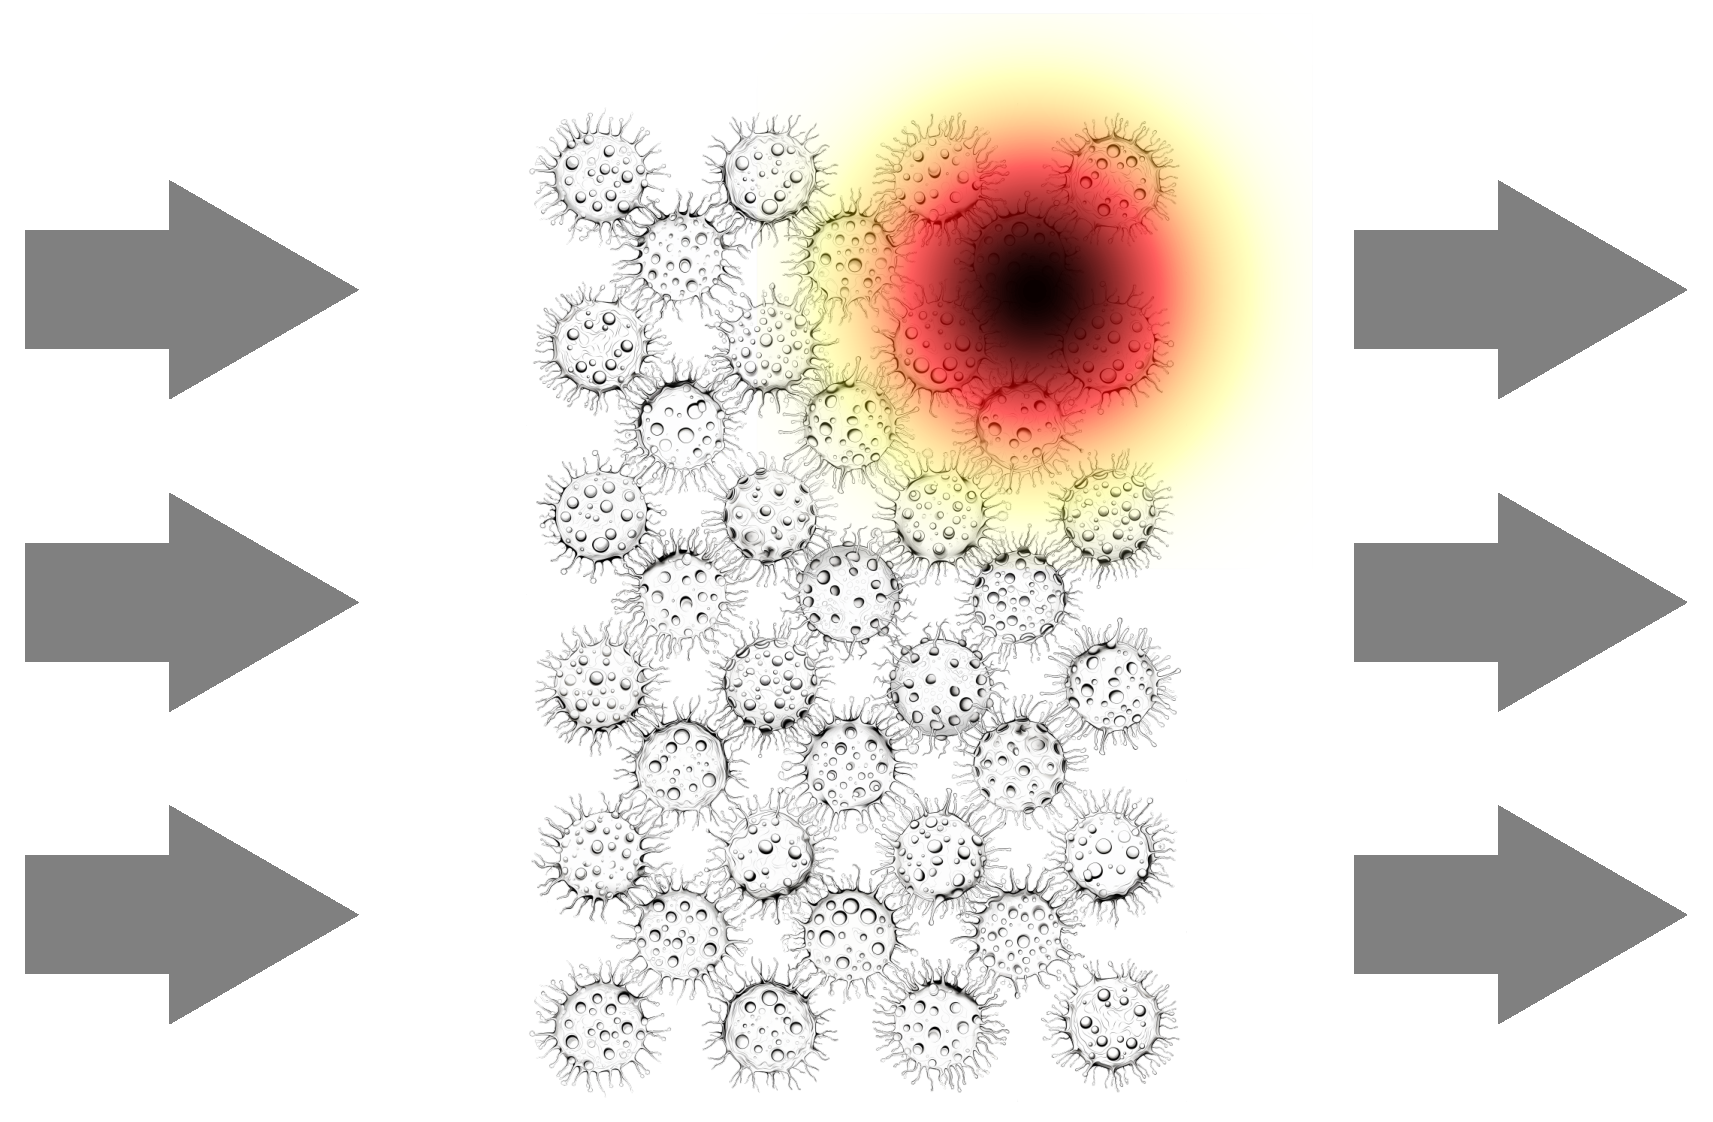
\includegraphics[width=0.35\textwidth]{parallel_heat_point.pdf}
		\\
		\hspace{1.1cm}
		Post Treatment
		\\
		\noindent
		\begin{subfigure}[b]{0.55\textwidth}
			\addtocounter{subfigure}{-1}
			\renewcommand\thesubfigure{\alph{subfigure}1}
			\centering
			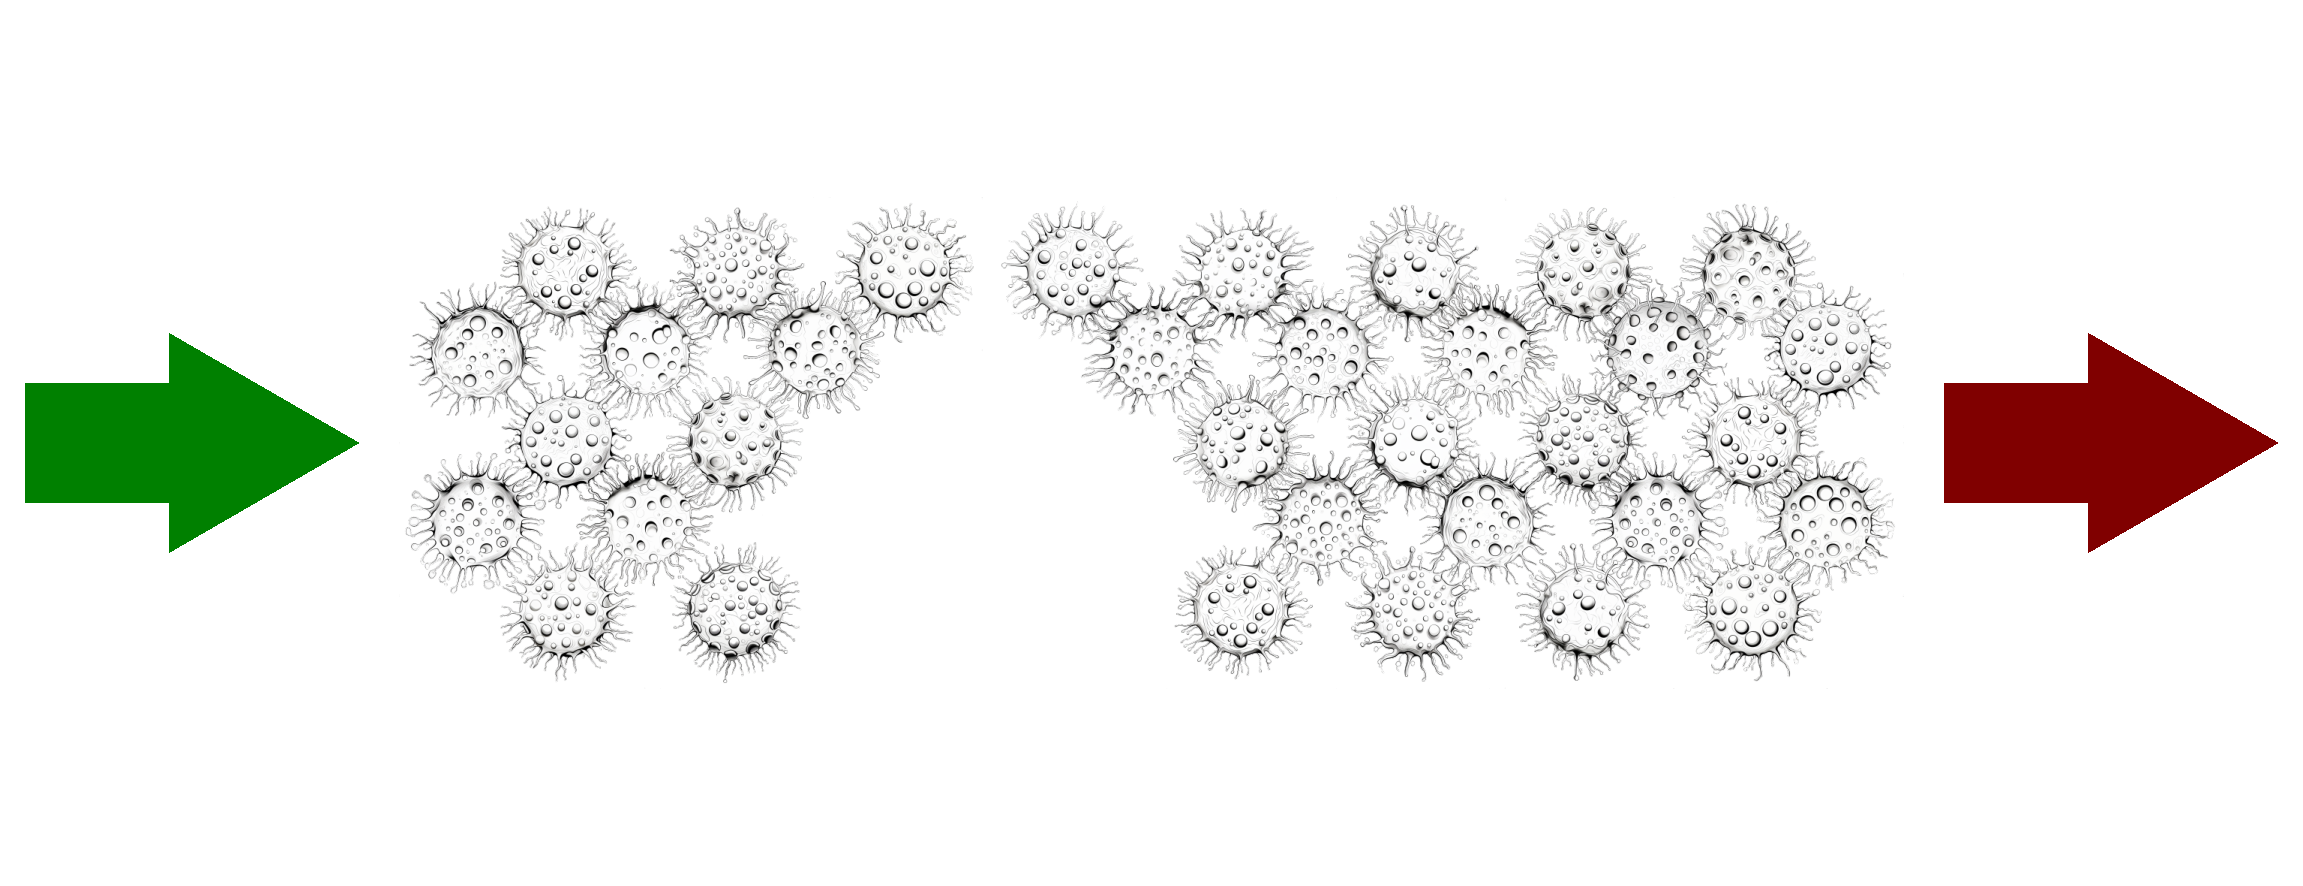
\includegraphics[width=\textwidth]{serial_heat_point_post.pdf}
			\vspace{0.5mm}
			\caption{Serial organ dies.}
		\end{subfigure}
		\vbar
		\begin{subfigure}[b]{0.35\textwidth}
			\addtocounter{subfigure}{-1}
			\renewcommand\thesubfigure{\alph{subfigure}2}
			\centering
			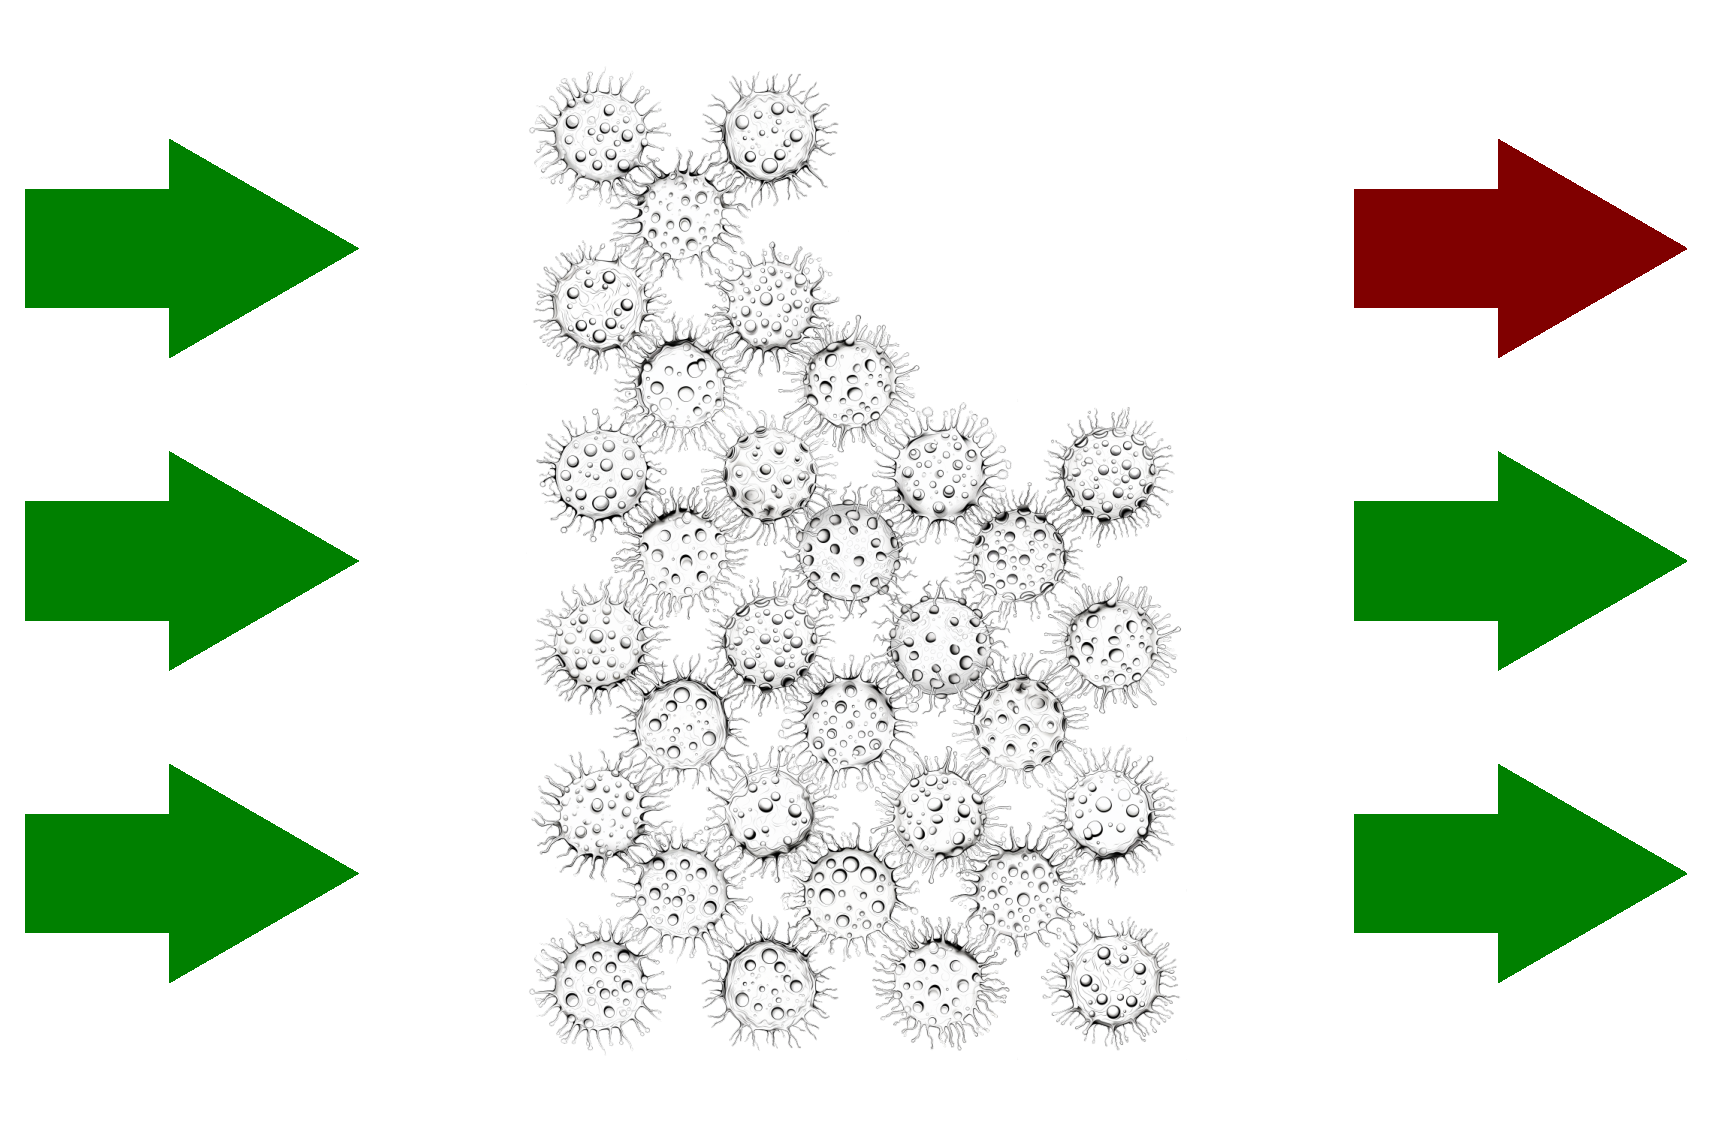
\includegraphics[width=\textwidth]{parallel_heat_point_post.pdf}
			\caption{Parallel organ survives.}
		\end{subfigure}	
	\end{subfigure}
	\vbar
	\begin{subfigure}[b]{0.48\textwidth}
		\caption{Irradiation of organs at risk with spread heat dose.}
		\label{fig:organ_radiation_square}
		\centering
		\vspace{3mm}
		\hspace{1.2cm}
		Treatment Dose
		\\
		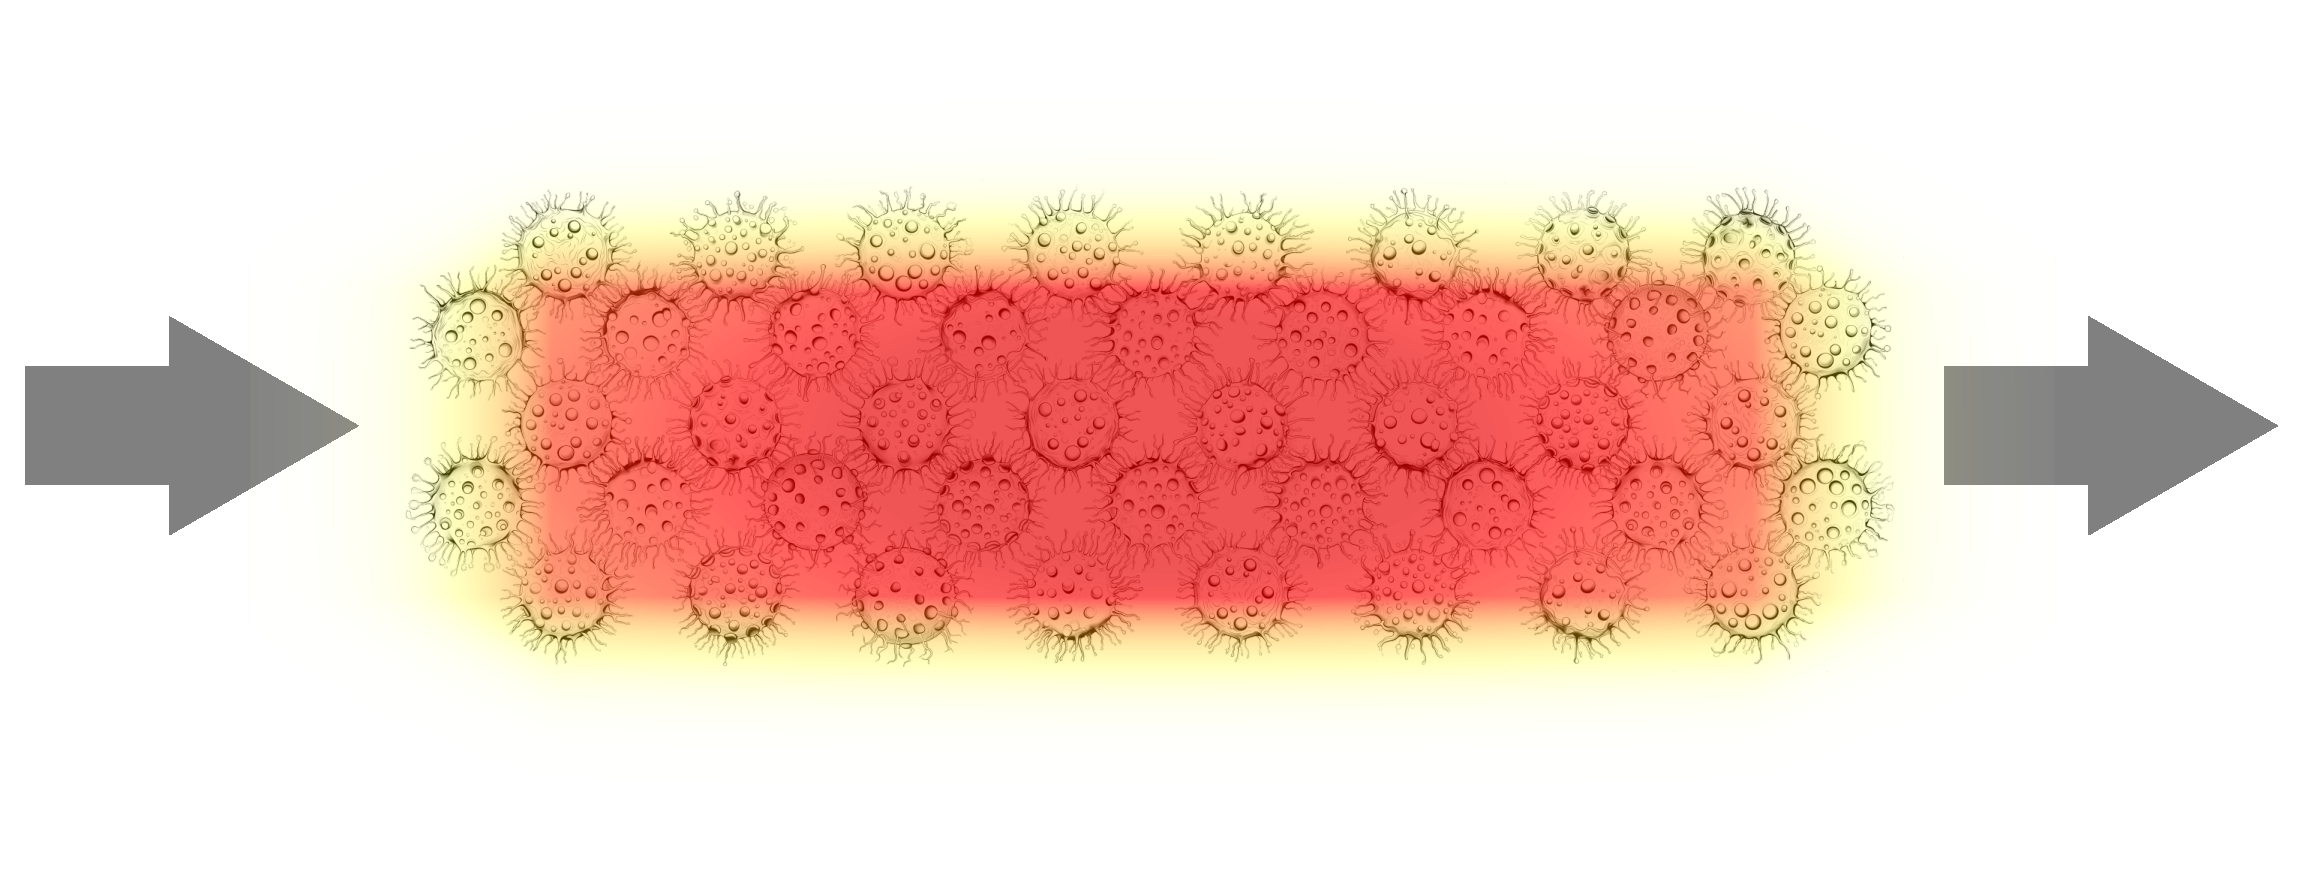
\includegraphics[width=0.55\textwidth]{serial_heat_square.pdf}
		\vbar
		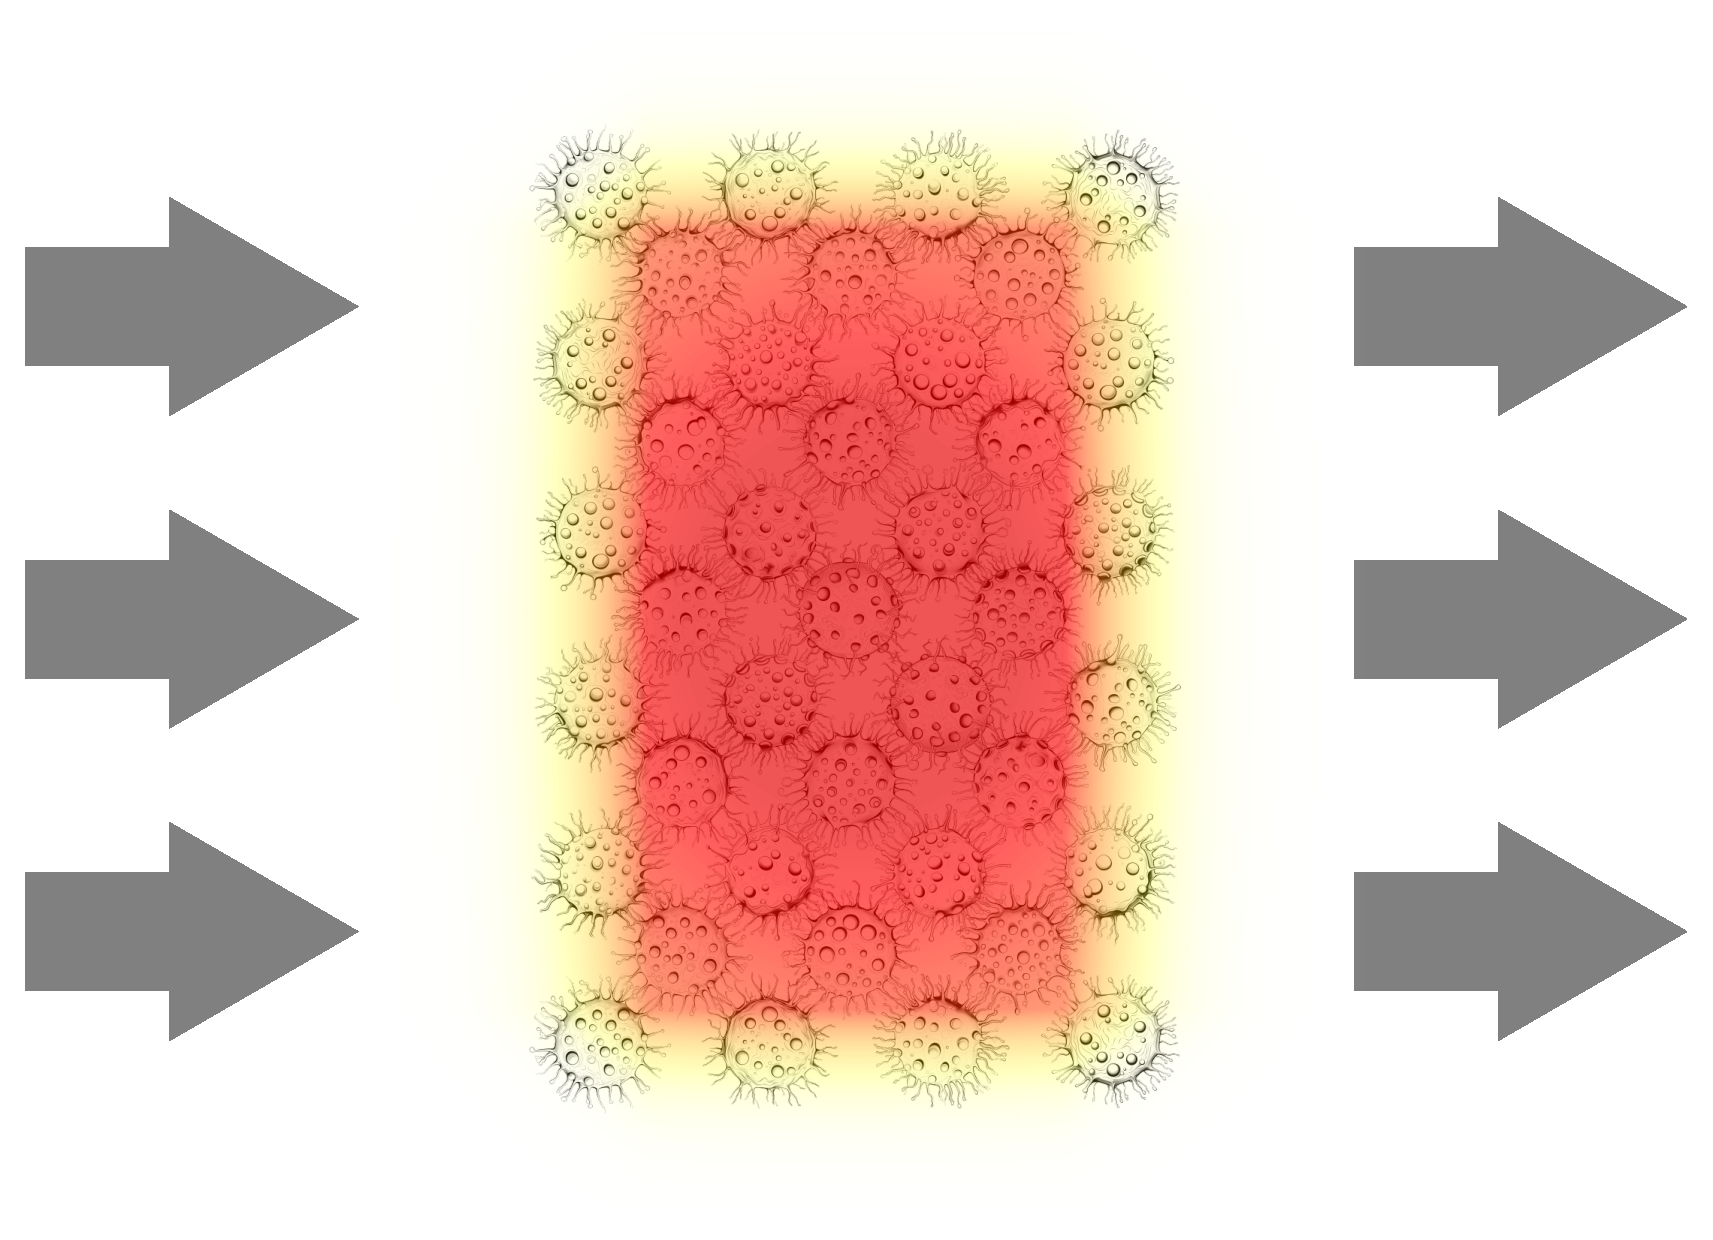
\includegraphics[width=0.35\textwidth]{parallel_heat_square.pdf}
		\\
		\hspace{1.1cm}
		Post Treatment
		\\
		\noindent
		\begin{subfigure}[b]{0.55\textwidth}
			\addtocounter{subfigure}{-1}
			\renewcommand\thesubfigure{\alph{subfigure}1}
			\centering
			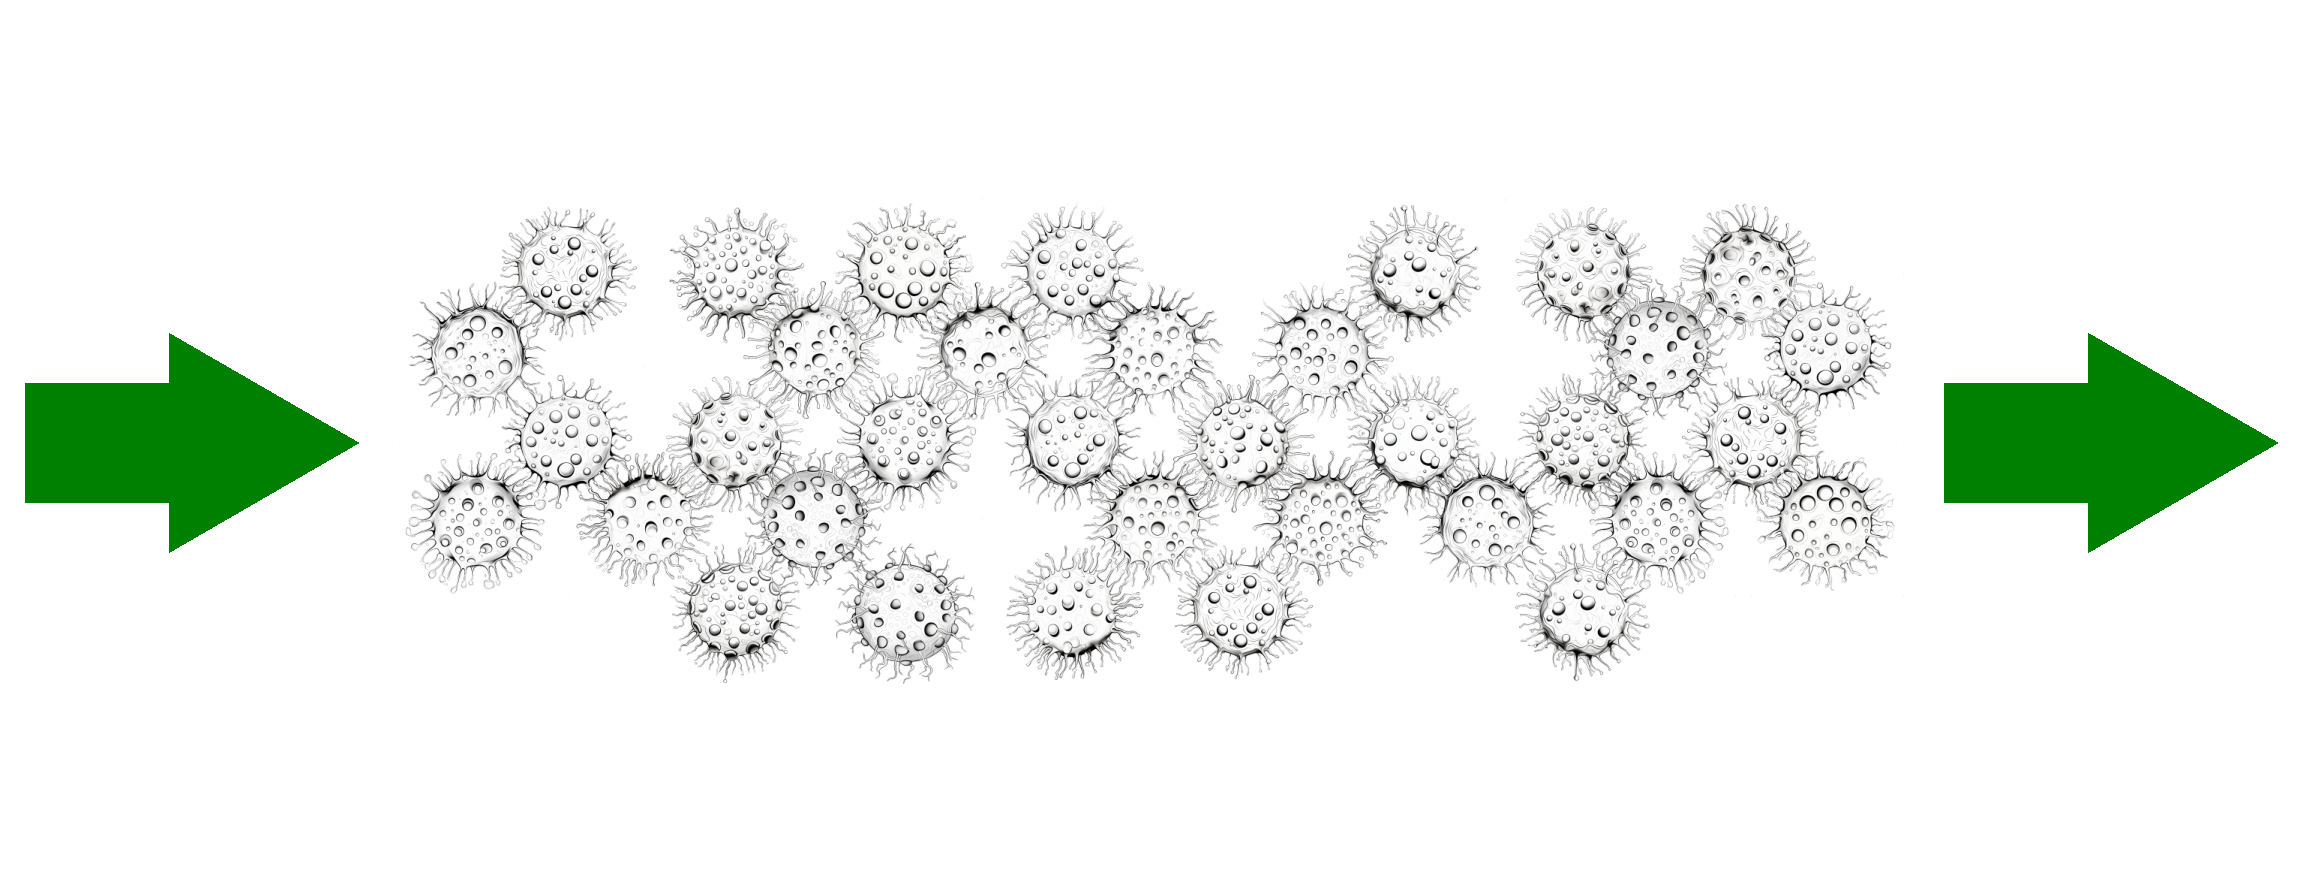
\includegraphics[width=\textwidth]{serial_heat_square_post.pdf}
			\vspace{0.5mm}
			\caption{Serial organ survives.}
		\end{subfigure}
		\vbar
		\begin{subfigure}[b]{0.35\textwidth}
			\addtocounter{subfigure}{-1}
			\renewcommand\thesubfigure{\alph{subfigure}2}
			\centering
			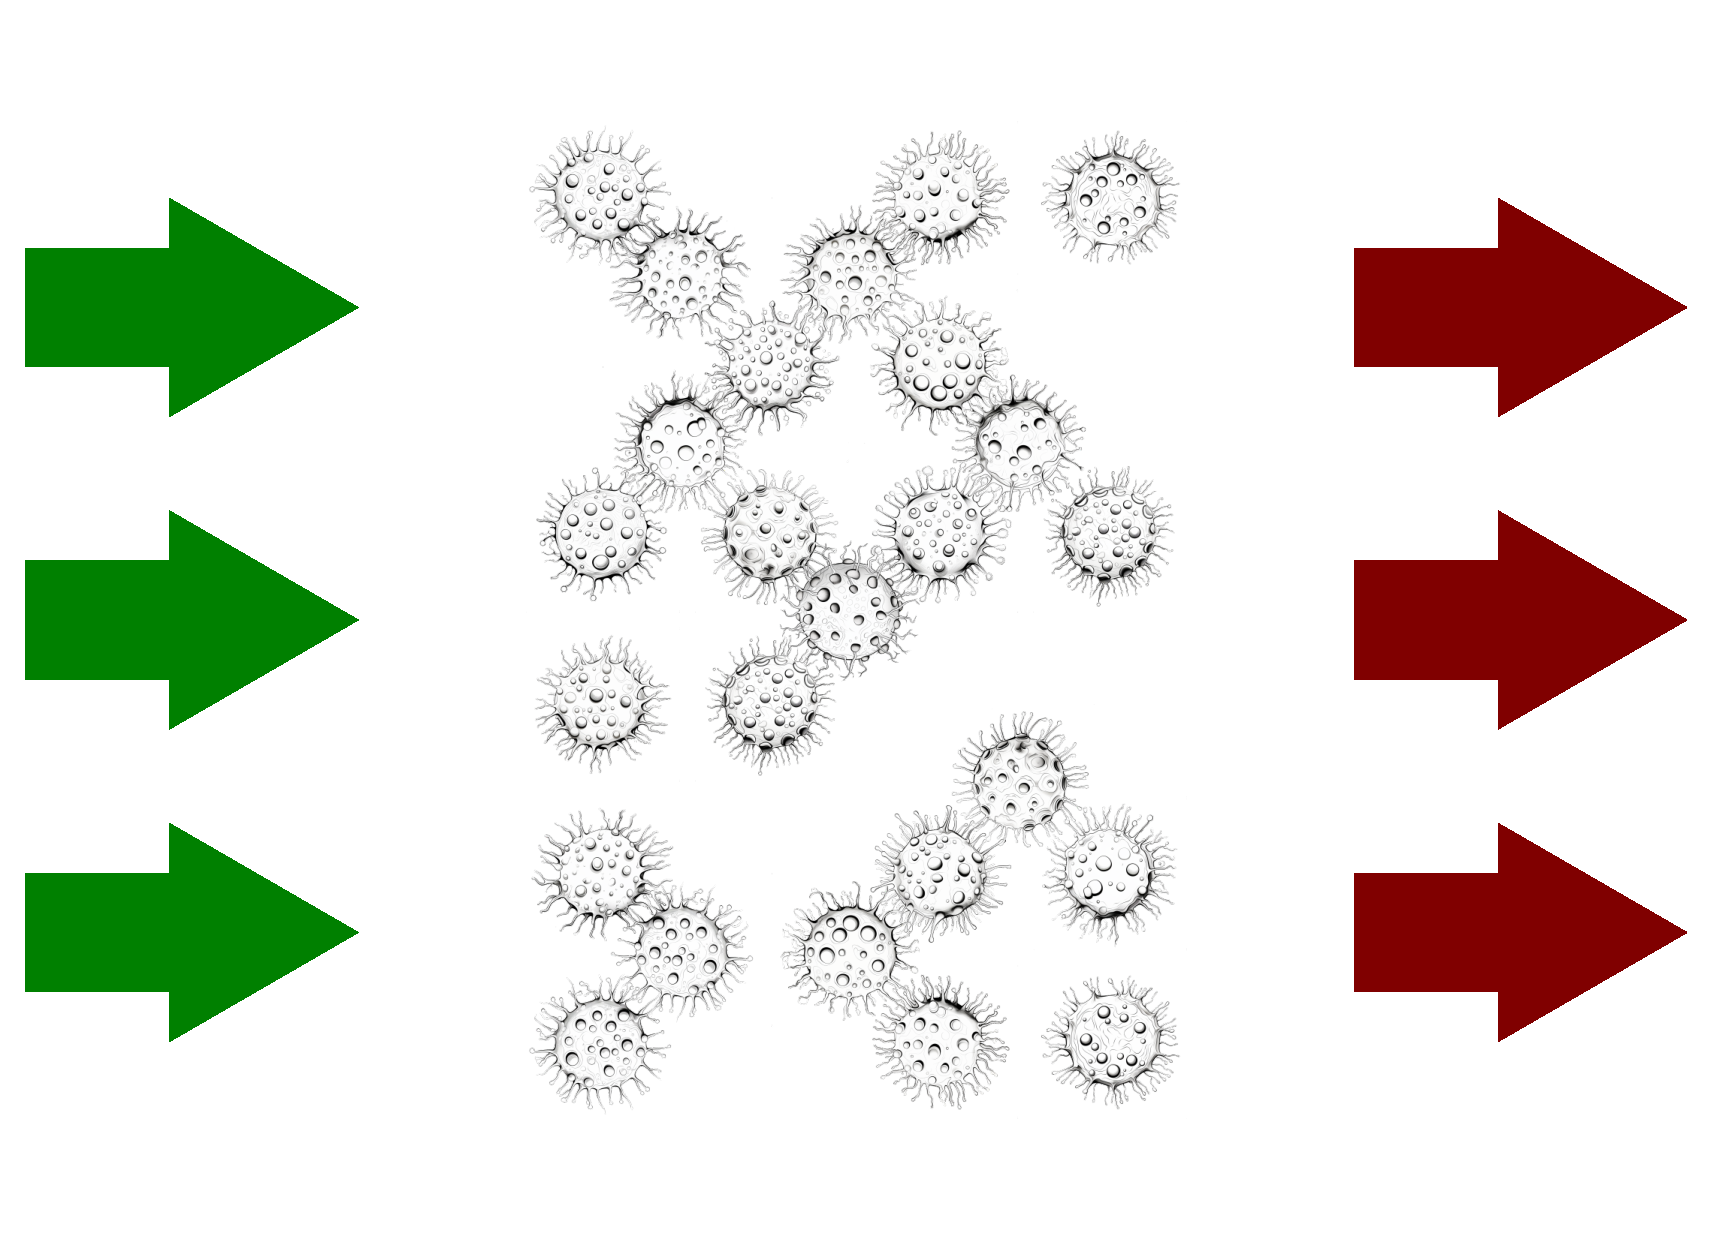
\includegraphics[width=\textwidth]{parallel_heat_square_post.pdf}
			\caption{Parallel organ dies.}
		\end{subfigure}	
	\end{subfigure}
	\addtocounter{subfigure}{-1}
	\caption{Irradiation type survival of organs serial-like and parallel-like.}
	\label{fig:serial_parallel_organ_radiation}	
\end{figure}

\subsection{Optimization Problem}

\paragraph{Ideal}
% minimize dose while reaching constraints

\paragraph{Practical}
% get as close as possible to meeting constraints
% building of cost function

\section{Dose Mimicking}
% principle
% => is a simpler problem
% => only works if dose to mimick is nearly acheaivable
% => can arise if machine is changing during treatment
% optim problem

\section{Optimization Algorithm Review for Dosimetry}
\subsection{Introduction}
% ArXiV paper

\subsection{Methods}
%Efficiently solving this optimization problem often involves designing the objective function to be convex, thereby providing a well-defined target for the optimization process.
%Gradient-based methods, Newtonian algorithms, or quasi-Newtonian algorithms are commonly employed for this purpose.
%We aim at benchmarking state-of-the-art open-source optimization algorithms for the specific task of radiotherapy dosimetry.

\subsection{Data}
% TG-119 \cite{AAPM-TG119}
\subsection{Objective function}
% details on the one used for this study
% => tested variations (p=1,2), changed importance factors, but v similar results
\subsection{Open-source Optimizers}
\paragraph{(Stochastic) Gradient Descent}
\paragraph{Conjugate Gradient}
\paragraph{Newton}
\paragraph{SLSQP}
\paragraph{RMSprop}
\paragraph{BFGS-based}
\subparagraph{Pure BFGS}
\subparagraph{L-BFGS}
\paragraph{Adam-based}
\subparagraph{Pure Adam}
\subparagraph{RAdam}
\subparagraph{NAdam}
\subparagraph{AdamDelta}
\subparagraph{Adamax}
\paragraph{Rprop}
\paragraph{Other optimizers variations}
%In addition, we also tested AdamW, Adagrad and ASGD.
%However, AdamW \& Adagrad behaved similarly to Adam, and ASGD behaved similarly to SGD.

\subsection{Results}
% 4 TGG-119 cases figures
\paragraph{Newton's method}
\paragraph{Best Algorithms}
\paragraph{LBFGS vs BFGS}

\subsection{Discussion}

	
	\chapter{Doses Relationship}
	\begin{chapterabstract}
		\lipsum[1-2]
	\end{chapterabstract}
	\clearpage
	\localtableofcontents
	% Full paper:
% https://github.com/pauldubois98/ESTRO2024/blob/main/full_paper.pdf
\section{Distance Between Doses}
In this section, we aim to establish a robust metric for quantifying the distance between different dose distributions.
Such a distance should provide a numerical comparison that reflects the clinical discrepancies between two dose distributions.
By developing a distance measure that captures these nuances, we can better evaluate and compare treatment plans.

\paragraph{A non-trivial task}
Quantifying the difference between two dose distributions, particularly regarding clinical impact, is inherently challenging.
This complexity arises because not all patient anatomy regions contribute equally to treatment outcomes.
Dose variations in critical structures may significantly influence clinical effects, while similar variations in less critical areas may have negligible impact.
Moreover, the potential for dose compensation (underdosing in one region counterbalancing overdosing in another) further complicates the development of a reliable metric for comparing dose distributions.
This compensatory effect is only sometimes applicable, making establishing a standardized method for assessing dose distribution clinical differences challenging.

\paragraph{Dose Evaluation}
To assess the quality of a dose distribution, dosimetrists primarily focus on DVHs as the key metric.
While they also consider aspects of the three-dimensional (3D) dose distribution, such as inter-structure dose gradients and the presence, number, and location of hot spots, their primary attention is directed towards the analysis of DVHs, which provide a comprehensive overview of dose coverage and sparing of organs at risk.

\subsection{Method}

\paragraph{Naive Doses Comparison}
The most straightforward method for comparing two dose distributions, thus defining a distance metric, is to perform a voxel-by-voxel comparison of the dose values.
However, this approach overlooks the inherent anatomical structure of the human body and the fact that not all voxels have the same clinical significance.
Consequently, even if the voxel-wise distance between two dose distributions is considerable, their overall clinical effects may still be similar.

\paragraph{Pathological example}
We constructed a simplified example, as illustrated in Figure \ref{fig:pathological_example}.
This hypothetical scenario involves a phantom model consisting of a homogeneous water-equivalent material containing a cubic planning target volume (PTV) and a cubic organ-at-risk (OAR).
Although this model lacks anatomical realism, it effectively highlights the limitations of using basic voxel-wise comparisons for dose evaluation.
It emphasizes the need for more sophisticated techniques to capture clinically relevant differences in dose distributions accurately.
\begin{figure}
	\centering
	\begin{subfigure}{0.44\linewidth}
		\includegraphics[width=\linewidth]{dose_distances_figures/example\_3d\_doses.pdf}
		\caption{3D visualization of the two doses on the phantom body.}
		\label{fig:pathological_example-3d_doses}
	\end{subfigure}
	\begin{subfigure}{0.55\linewidth}
		\includegraphics[width=\linewidth]{dose_distances_figures/example\_bixels.pdf}
		\caption{2D view of the bixels activation of the two doses.}
		\label{fig:pathological_example-bixels}
	\end{subfigure}
	\begin{subfigure}{0.75\linewidth}
		\includegraphics[width=\linewidth]{dose_distances_figures/example\_dvh.pdf}
		\caption{Dose-Volume Histograms of the two doses on the phantom body.}
		\label{fig:pathological_example-dvh}
	\end{subfigure}
	\caption{Example of two doses that have the same clinical effect (measured from the DVHs), but very different voxel-wise dose values.}
	\label{fig:pathological_example}
\end{figure}

\subsubsection{Doses Samples}
We assessed the efficacy of our proposed method for comparing radiation doses using the TG-119 Prostate case, a well-established benchmark for evaluating radiation therapy plans \cite{AAPM-TG119}.
The TG-119 dataset includes predefined dose objectives, which we utilized to formulate our cost function.
We performed optimizations with different weight assignments applied to each constraint to generate varying treatment dose distributions for the same patient case under identical constraints.

\subsubsection{Distances Between Doses}
\paragraph{Comparing Doses Voxel-wise}
%If two doses are very close together, than voxel-wise comparison is a good measure: we can suppose that the global repartition is similar, and voxel-wise comparison is a good tool to compare local distribution of the dose.
%Mathematically, we take $\textbf{d}$, the dose voxel-wise, and define the distance between $\textbf{d}_1$ and $\textbf{d}_2$ as the norm of the difference: $\sum_{v \in \mathcal{V}} \abs{d_1(v)-d_2(v)}$, $v$ being voxels in the set of voxels of interest $\mathcal{V}$, and $d_i(v)$ the value of the dose $d_i$ on voxel $v$ (we usually write $\abs{ \textbf{d}_1 - \textbf{d}_2}$, implicitly summing over voxels).
%
%However, if two regions of equal volume, located in the same structure have their dose values swapped, the voxel-wise difference would be high, although clinically, the two doses are equivalent.
%Thus, voxel-wise distance is not a good measure between doses for comparing global distribution.

\paragraph{Comparing Dose Volume Histogram Curves}
%We propose to compare the curves on the Dose Volume Histogram (DVH).
%We have one curve for each structure; we define the distances between doses for each structure, and in the end, we sum up for all structures to end up with a single scalar distance between two doses.

\subparagraph{Discrete DVH Approximation}
%The DVH is obtained after sorting the voxel-wise dose of the structure:
%Let $\textbf{d} \left[s\right]$ bet the voxel-wise dose of the structure $s$ (therefore, a list, of length $n(s)$, the number of voxels that belong to the structure).
%Let $\dot{\textbf{d}\left[s\right]}$ be the list above in descending order (i.e. $\dot{\textbf{d}\left[s\right]}_i > \dot{\textbf{d}\left[s\right]}_j$ if $0 < i < j \leq n(s)$).
%Then, the DVH of $s$ can be approximated by the continuous line composed of the segments linking the following points:
%$\left( \dot{\textbf{d}\left[s\right]}_i, i/n(s) \right) \quad 0 < i \leq n(s)$.
%Since we compute the dose voxel-wise, we may only have an approximation of the DVH.
%However, in practice, most structures of interest have more than a hundred voxels, which makes the DVH approximation very precise.
%
%Since we draw one curve per structure of interest, this capture some of the importance of voxel over others.
%In fact, when analyzing a dose, doctors look at the dose volume (voxel-wise), but they also take a close look at the DVHs; this is an incentive that DVHs should contain meaningful information.
%
%To measure how different two DVH curves, we can imagine several techniques:
%\begin{itemize}
%	\item Fréchet distance (treating DVHs as curves in a 2D space)
%	\item Hausdorff distance (treating DVHs as 1D manifolds in a 2D space)
%	\item Wasserstein distance (treating DVHs as probability distributions)
%	\item Kolmogorov-Smirnov test (treating DVHs as probability distributions)
%	\item Total variation between curves (treating DVHs as functions)
%\end{itemize}
%We tried all the distances above, but propose to retain only the one giving the best results.

\subparagraph{Fréchet Distance}
%We can look at DVH curves as lines in $\R^2$ \ \footnote{(Or, in the case of our voxel-wise dose approximation, poly-lines in $\R^2$.)}.
%In this case, the Fréchet distance is a well known measure of similarity between two curves, and is particularly used for poly-lines \cite{Efrat2002}.
%It measures the minimum distance that must be covered by a particle moving along two curves simultaneously.
%In our case, these curves are the DVH curves of two radiation doses.
%The Fréchet distance is therefore, a metric of similarity between two curves.
%
%Formally, if $P$ and $Q$ are the curves being compared, $\gamma$ being a parametrization defined on the interval $\left[ 0,1 \right]$, $P(\gamma(t))$ and $Q(\gamma(t))$ the positions of a particle along curves $P$ and $Q$, respectively, at time $t$, the Fréchet distance is then defined as:
%$$d_{\text{Fréchet}}(P,Q) = \inf_{\gamma}{ \max_{t \in \left[ 0,1 \right]} d(P(\gamma(t)), Q(\gamma(t)))}$$
%
%Now, adapting this to DVH curves:
%Let $\mathcal{C}_A$ and $\mathcal{C}_B$ represent the (discrete) DVH curves of two doses.
%Let them respectively be consisting of line segments joining the series of points $\left\lbrace \mathcal{C}_A(i) = (d_i, v_i), \ 1 \leq i \leq n_A \right\rbrace $ and $\left\lbrace \mathcal{C}_B(j) = (\tilde{d}_j, \tilde{v}_j), \ 1 \leq j \leq n_B \right\rbrace $; where $d_i$ and $\tilde{d}_j$ denote the dose levels, $v_i$ and $\tilde{v}_j$ represent the corresponding volumes, and $n_A$ and $n_B$ are the number of points forming $\mathcal{C}_A$ and $\mathcal{C}_B$\footnote{Since we are always comparing two DVH curves of the same structure, we always have $n_A = n_B$.}.
%
%The Fréchet distance is the infimum of all possible traversal times.
%The curves being discrete line segments, we can express the Fréchet distance as:
%
%$$d_{\text{Fréchet}}(\mathcal{C}_A, \mathcal{C}_B) = \min_{\substack{j: \llbracket 1, n_A \rrbracket \to \llbracket 1, n_B \rrbracket \\ j \nearrow \ (j \text{ increasing})}} \sum_{i=1}^{n_A} dist\left( \mathcal{C}_A(i), \mathcal{C}_B(j(i)) \right)$$
%$$\text{where } dist\left( \mathcal{C}_A(i), \mathcal{C}_B(j(i)) \right) = \sqrt{(d_i-\tilde{d}_{j(i)})^2 + (v_i-\tilde{v}_{j(i)})^2}$$
%%$$\text{i.e.: } d_{\text{Fréchet}}(\mathcal{C}_A, \mathcal{C}_B) = \min_{\substack{j: \llbracket 1, n_A \rrbracket \to \llbracket 1, n_B \rrbracket \\ j \nearrow \ (j \text{ increasing})}} \sum_{i=1}^{n_A} \sqrt{(d_i-\tilde{d}_{j(i)})^2 + (v_i-\tilde{v}_{j(i)})^2}$$
%
%Here, $j$ represents a (discrete) a parametrization, and $dist\left( \mathcal{C}_A(i), \mathcal{C}_B(j(i)) \right)$ is the distance between points $\mathcal{C}_A(i)$ and $\mathcal{C}_B(j(i))$.
%
%The main drawback of this distance measure is that it is computationally expensive, especially for structures with many voxels.
%Thus, we had to couple it with an algorithm for curve simplification: the Ramer–Douglas–Peucker algorithm \cite{PRASAD2012843}.
%We used the Ramer–Douglas–Peucker algorithm with $\varepsilon = 0.05$.
%After testing on a few curves, using this algorithm made calculations 3-5 times faster, while affecting the value of the Fréchet distance by less than $0.5\%$.
%It is therefore used in the results presented thereafter.

\subparagraph{Hausdorff Distance}
%The Hausdorff distance is another metric of similarity between two curves \cite{Henrikson1999CompletenessAT}.
%It is defined as the maximum distance between any point on one curve to its closest point on the other curve.
%Formally, let $X$ and $Y$ be two non-empty sets;
%the Hausdorff distance between $X$ and $Y$, denoted as $d_\text{Hausdorff}(X, Y)$, is defined as:
%$$d_\text{Hausdorff}(X, Y) = \sup_{x \in X}\inf_{y \in Y} {dist(x, y)}$$
%where $dist(x, y)$ is the distance between points $x$ and $y$.
%
%In our analysis, we treat the DVH curves as sets of points in a 2D space ($\R^2$) and use the Hausdorff distance to measure the difference between them.
%Using the same notation for DVH curves $\mathcal{C}_A$ and $\mathcal{C}_B$ as before, the discrete Hausdorff distance can be computes as follows:
%$$d_\text{Hausdorff}(\mathcal{C}_A, \mathcal{C}_B) = \max_{i \in \llbracket 1,n_A \rrbracket} \min_{y \in \mathcal{C}_B} {dist(\mathcal{C}_A(i), y)}$$
%with $\mathcal{C}_B = \left\lbrace \left( (1-\lambda) \tilde{d}_j + \lambda \tilde{d}_{j+1}, (1-\lambda) \tilde{v}_j + \lambda \tilde{v}_{j+1} \right) \mid \lambda \in \left[ 0,1 \right], j \in \llbracket 1, n_B-1 \rrbracket \right\rbrace $, and $dist$ the 2D distance (as before).

\subparagraph{Wasserstein Distance}
%The Wasserstein distance, also known as the Earth Mover's Distance, is a metric that quantifies the difference between two probability distributions \cite{OLKIN1982257}.
%
%Formally, letting $\mu$ and $\nu$ be two probability distributions defined on a metric space $X$;
%the Wasserstein distance, denoted as $d_{\text{Wasserstein}}(\mu, \nu)$, is defined as the infimum cost of transporting the mass from the distribution $\mu$ to the distribution $\nu$, where the cost is determined by the distance metric $dist$ on $X$.
%That is:
%$$d_{\text{Wasserstein}}(P, Q) = \inf_{\gamma \in \Gamma(\mu, \nu)} E_{(x,y) \sim \gamma} \left[ dist(x, y) \right]$$
%where $\Gamma(\mu, \nu)$ is all possible joint distributions $\gamma(x, y)$ with marginals $\mu$ and $\nu$.
%
%In our analysis, we treat the DVH curves as probability distributions and use the Wasserstein distance to measure the difference between them.
%The main advantage of this distance measure is its ability to capture both local and global differences between the curves.
%However, it can be computationally expensive, especially when dealing with DVH of large structures.

\subparagraph{Kolmogorov-Smirnov Distance}
%Another distance metric that can be used to compare two dose volume histogram (DVH) curves is the Kolmogorov-Smirnov (KS) distance \cite{Stephens1974}.
%The KS distance measures the maximum vertical distance between the two curves and is particularly useful when comparing two non-parametric distributions, such as the DVH curves.
%
%Mathematically, let the two DVH curves be described by $f$ and $g$ (from the dose domain to the volume ratio domain), we then have the KS distance $d_{KS}$ given by:
%$$d_{KS} = \sup_{x \in \R^+} \abs{f(x)-g(x)}.$$
%In our case of discrete DVH, $f$ and $g$ will be linear by segment continuous functions from $\R^+$ to $\left[ 0,1 \right]$ (with value zero above the maximal dose).

\subparagraph{Total Variation Distance}
%Finally, we propose a distance metric that computes the integral of the absolute difference between the two DVH curves.
%This distance measure is simple to compute and provides a good balance between capturing local and global differences between the curves \cite{Chatterjee2007}.
%Moreover, it is computationally efficient and can handle large structures with many voxels.
%It is the one that gave the best results, hence, we chose this distance for our analysis.
%
%Initially, the total variation distance measures the integral of the absolute difference between two dose volume histogram (DVH) curves.
%The dose is (theoretically) unbounded, while the relative volume is bounded (0-100\%).
%We preferred to integrate over a bounded volume instead of an unbounded dose.
%Hence, we flipped the $x$ and $y$ axes before integrating the absolute dose difference on the range $\left[ 0,1 \right]$; that is, we have the dose on the $y$ axis, and the volume on the $x$ axis.
%
%Mathematically, standard DVHs are given by $V: \R^+ \to \left[ 0,1 \right]$.
%With two DVHs $V(d)$ and $\tilde{V}(d)$, the total variation will be
%$$d_{\text{TotalVariation}} = \int_{0}^{+\infty} \abs{V(x)-\tilde{V}(d)}.$$
%However, we choose to express DVHs with dose as a function of volume, that is $D: \left[ 0,1 \right] \to \R^+$.
%With two DVHs $D(v)$ and $\tilde{D}(v)$, the total variation will be
%$$d_{\text{TotalVariation}} = \int_{0}^{1} \abs{V(x)-\tilde{V}(d)}.$$
%The value of the integral should not change (in theory); we prefer to integrate over a finite domain ($\left[ 0,1 \right]$) than over an unbounded one ($\R^+ = \left[ 0,+\infty \right[$).
%
%An illustration of the differences between classical DVH and after swapping $x$ and $y$-axes is available on figure \ref{fig:dose_volume_difference}.
%The two doses compared were optimized on the TG-119 fake prostate case with different weights (1 and 3) on the PTV objective.
%
%\begin{figure}
%	\centering
%	\includegraphics[width=0.95\textwidth]{dose_distances_figures/dose\_volume\_difference}
%	\subfloat[\label{fig:dose_volume_difference-normal} Classical DVH (dose on the $x$-axis)]{\hspace{1\linewidth}}
%	
%	\centering
%	\includegraphics[width=0.95\textwidth]{dose_distances_figures/dose\_volume\_difference-flipped}
%	\subfloat[\label{fig:dose_volume_difference-flipped} Flipped axes DVH (volume on the $x$-axis)]{\hspace{1\linewidth}}
%	
%	\caption{DVHs: Comparison of classical and flipped axes styles.}
%	\label{fig:dose_volume_difference}
%\end{figure}
%
%We observe (on fig. \ref{fig:dose_volume_difference}) that the difference between DVHs is less noisy (it fluctuates less) when we have the dose on the $x$-axis.
%This suggest lower numerical error, and is therefore another incentive to have the volume as the $x$-axis.
%
%The calculation of the total variation distance is computationally efficient, requiring only $\mathcal{O}(n_s)$ operations for each structure, where $n_s$ is the number of voxels in the structure of interest $s$.
%Overall, it provides a good balance between capturing local and global differences of DVH curves.



\subsection{Results}
\subsubsection{Dose Distances Comparison}
%For each constraint, we perform an optimization with all weights set to $1$, but one, that we sequentially set to $3$, $10$, $100$.
%This gives us 18 doses that we can compare.
%We can calculate the pairwise distance between each pair of doses, for each of the distance techniques described above.
%Considering each optimized dose as a node, we can create a graph for each of the defined distance; and calculating the pairwise distance is equivalent to calculating the adjacency matrix if the associated dense graph.
%See figure \ref{fig:pairwise_distances} for a comparison of the adjacency matrices.
%\begin{figure}
%	\centering
%	\includegraphics[width=\textwidth]{dose_distances_figures/pairwise\_distances.pdf}
%	\caption{Pairwise distances between doses\\(with different distances calculation method)}
%	\label{fig:pairwise_distances}
%\end{figure}
%
%Ideally, we want a new distance that:
%\begin{itemize}
%	\item matches the voxel distance when voxel distance is low
%	\item remains small in some cases of a high voxel distance: when the clinical meaning og the two doses is the same, despite being voxel-wise (very) different
%\end{itemize}
%
%Observing pairwise distances on fig. \ref{fig:pairwise_distances}, we have that:
%\begin{itemize}
%	\item Frechet and Haussdorff are very similar to voxel-wise; we interpret them as being too sensitive.\\
%	They are therefore not suitable for our purpose.
%	\item Kolmogorov-Smirnov degenerates; it probably captured some noise due to approximation in the DVH calculation (small numerical error).\\
%	It is therefore not suitable for our purpose.
%	\item Wasserstein and Total variation seem to produce acceptable results.\\
%	We therefore chose to continue studying these two distances.
%\end{itemize}

\subsubsection{Link between Total Variation and Wasserstein}
%One may remark that the adjacency matrices for Wasserstein and Total Variation are very similar.
%And in fact, since we used Earth moving distance (Wasserstein with $p=1$), there is an equivalence between the two measures.
%More precisely, the total variation distance can be seen as a special case of the Wasserstein distance.
%
%The Wasserstein distance, also known as the earth mover's distance, is a metric that quantifies the distance between two probability distributions.
%Given two probability distributions $X$ and $Y$ with CDFs $F$ and $G$, the Wasserstein distance between them is defined as:
%$$W_p(F,G) = \inf_{\pi \in \Pi(F,G)} \left( \iint_{x,y \in \mathbb{R}^2} \abs{x-y}^p d\pi(x,y) \right)^{1/p}$$
%
%On the other hand, the total variation distance between two curves $F$ and $G$ is defined as:
%$$\text{TotalVariation}(F, G) = \int_{x \in \R} \abs{F(x) - G(x)} dx$$
%
%The Wasserstein distance is equivalent to the total variation distance for $p=1$:
%$$W_1(F, G) \equiv \text{TotalVariation}(F, G).$$
%
%In the end, the only difference should be numerical error.

\subsubsection{Bounding of Total Variation and Voxel Distance}
%It is possible to bound the total variation distance with the Voxel Distance.
%The other way around, however, is impossible, as shown with the example int the introduction (where two doses have close to identical DVHs, but very different Voxel distances).
%
%We will bound the total variation of one DVH, hence being generalizable to the sum of all DVHs total variation distances.

\paragraph{Definitions}
%Let $\mathcal{S}$ be the structure of interest, and $v_\mathcal{S}$ the set of voxels associated to the structure, with $n_\mathcal{S} = \abs{v_\mathcal{S}}$ the number of voxels.
%Let $d$ and $\tilde{d}$ be the two doses to be compared.

\paragraph{Sorting lists}
%\begin{lemma}
%	\label{lemma:sorting_lists}
%	Let $\dot{l}, l^* \in \R^n$. Let $\dot{l}$ be sorted and $\dot{l^*} \in \R^n$ be sorted version of $l^*$.
%	Then, we have:
%	$$\abs{\dot{l} - l^*} \geq \abs{\dot{l} - \dot{l^*}}$$
%\end{lemma}
%\begin{proof}
%	Suppose $a<b$ and $c<d$, and WLOG, $a\leq c$.\\
%	We have $\abs{a-d} = \abs{a-c}+\abs{c-d}$
%	so $\abs{a-d}+\abs{b-c} = \abs{a-c}+\abs{c-d}+\abs{b-c}$
%	using triangle inequality ($\abs{c-d}+\abs{b-c} \geq \abs{b-c}$):
%	$\abs{a-d}+\abs{b-c} \leq \abs{a-c}+\abs{b-d}$.\\
%	Thus, with $\dot{l}$ sorted, swapping elements $l_i$ and $l_j$ ($i<j$) of $l^*$ decreases $\abs{\dot{l} - l^*}$ if $l_i \geq l_j$.
%	Now, bubble sort on $l^*$, we obtain $\dot{l^*}$ doing only permutations satisfying the condition just stated.
%	
%	Hence, we obtain $\abs{\dot{l} - l^*} \geq \abs{\dot{l} - \dot{l^*}}$ at the end of the bubble sort.
%	\qed
%\end{proof}
%\begin{corollary}
%	\label{corollary:sorting_lists}
%	Let $l, l^* \in \R^n$. Let $\dot{l},\dot{l^*} \in \R^n$ be sorted version of $l, l^*$.
%	Then: $$\abs{l - l^*} \geq \abs{\dot{l} - \dot{l^*}}$$
%\end{corollary}
%\begin{proof}
%	The order in which we perform $\abs{l - l^*} = \sum_{k=1}^{n} \abs{l_k-l^*_k}$ can be chosen, so $\abs{l - l^*} = \sum_{k=1}^{n} \abs{l_{\sigma(k)}-l^*_{\sigma(k)}}$ (with $\sigma$ a permutation of $\llbracket 1,n \rrbracket$).
%	Taking $\sigma$ such that $l_{\sigma(i)} \leq l_{\sigma(j)}$ for $i<j$ and using lemma finishes the proof.
%	\qed
%\end{proof}

\paragraph{Proof Outline}
%Suppose the voxel-wise difference is $\varepsilon$-small (i.e. $\abs{d_i-\tilde{d}_i} < \varepsilon$).
%Then, the total variation of the unsorted vector doses is $\abs{d-\tilde{d}} < n_\mathcal{S} \varepsilon$.
%Let $\dot{d}$ be sorted $d$ and $\dot{\tilde{d}}$ be sorted $\tilde{d}$.
%Then, by Corollary \ref{corollary:sorting_lists}, we have:
%$\abs{\dot{d}-\dot{\tilde{d}}} \leq \abs{d-\tilde{d}} < n_\mathcal{S} \varepsilon$.
%
%Therefore, if $d$ and $\tilde{d}$ are sufficiently close, $\varepsilon \to 0$ and $\abs{\dot{d}-\dot{\tilde{d}}} \to 0$.

\paragraph{Conclusion}
%Thus, voxel-wise very close doses distributions will also have close DVHs distances, which ensure DVHs distances are non-degenerative.

\subsubsection{Distances Distribution Comparison}
%\begin{figure}
%	\centering
%	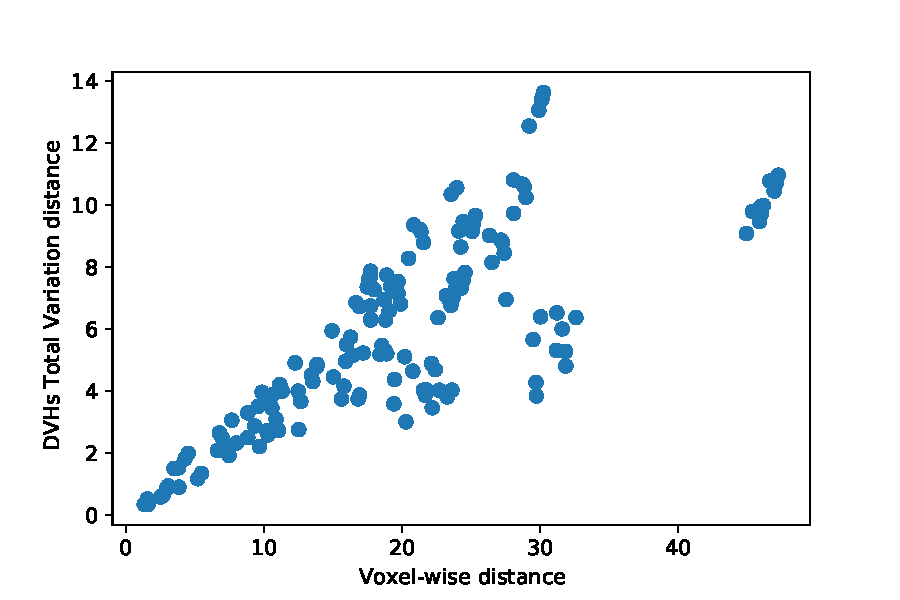
\includegraphics[width=0.49\textwidth]{dose_distances_figures/TotalVariation-Voxelwise.pdf}		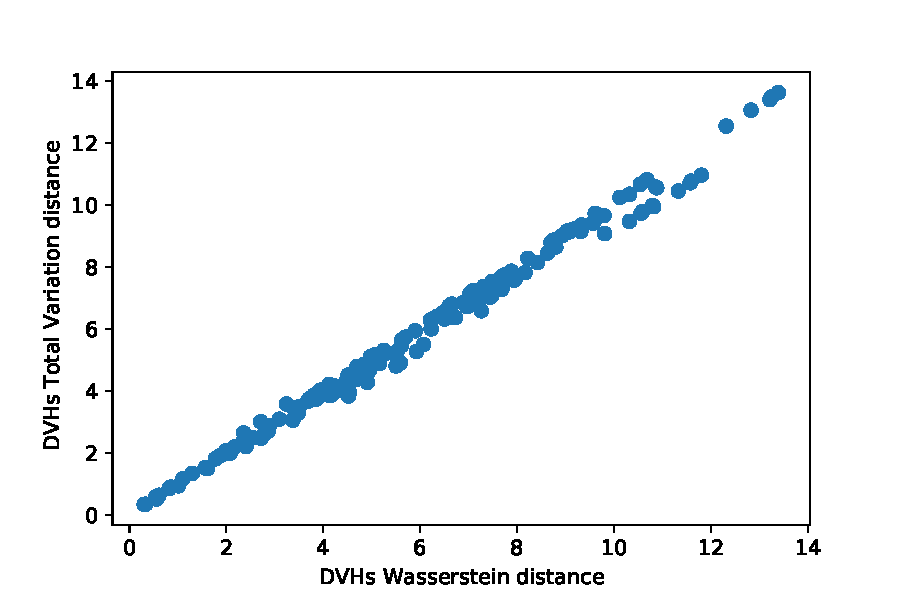
\includegraphics[width=0.49\textwidth]{dose_distances_figures/TotalVariation-Wasserstein.pdf}
%	\subfloat[\label{fig:TotalVariation-Voxelwise} DVHs Total Variation vs Voxel-wise]{\hspace{.5\linewidth}}
%	\subfloat[\label{fig:TotalVariation-Wasserstein} Total Variation vs Wasserstein]{\hspace{.5\linewidth}}
%	\caption{Comparing Distances}
%\end{figure}

\paragraph{Comparing Total Variation and Voxel-wise}
%The bounding of the total variation DVH distance in terms of voxel-wise distance is clear on figure \ref{fig:TotalVariation-Voxelwise} (there is a linear upper bound to the scatter plot).
%However, we can remark that some pair of distances are closer in terms of DVH than we imagined using just the voxel-wise distance; hence proving the necessity to analyze further than just the voxel-wise comparison.

\paragraph{Comparing Total Variation and Wasserstein}
%We observe (on figure \ref{fig:TotalVariation-Wasserstein}) that the two DVH distances are almost perfectly proportional.
%This was expected as they are equivalent mathematically, we only swapped axis of integration in the total variation (hence, the small fluctuations).



\subsection{Discussion}
%In this article, a novel metric for comparing radiation doses is introduced.
%This metric has the advantage of being insensitive to dose changes in some regions if being compensated in another region, which was the intended goal.
%This metric can be useful in several applications, such as dose mimicking and early stopping time for fluence map optimization optimization.
%
%However, there are some limitations to this distance metric.
%One drawback is that it does not capture spatial distribution, which can be a problem in some cases.
%There may be some pathological examples where the DVHs are similar, but the clinical interpretation is different.
%Other factors, such as the distribution of the dose within the target area or the surrounding tissues, can also play a crucial role in determining the effectiveness of the treatment.
%For example, if two doses have the same amount of high dose, one spread in several small high dose regions, and the other having one large high dose region, then the DVH could look alike, while doctors will interpret the two doses differently.
%These types of edge cases are, however, extremely rare in practice.
%We still advise, for critical cases, to use the voxel invariant metric in conjunction with other techniques to obtain a comprehensive evaluation of radiation doses.
%
%When comparing two different doses, a large distance between them could indicate a significant difference in the intensity or frequency of the treatment, but this does not necessarily mean that one dose is better than the other.
%The effectiveness of a dose also depends on several other factors such as the individual patient's characteristics, medical history, and response to the treatment.
%Thus, simply looking at the distance between doses may not provide an accurate picture of which dose is superior or more effective in a particular case.
%It is essential to consider all relevant factors when evaluating the efficacy of a treatment dose.
%
%Overall, our dose comparison technique is a promising tool.
%While it has some limitations, it can be a valuable addition to the arsenal of techniques used by radiation oncologists and medical physicists to optimize treatment plans and improve patient outcomes.

\paragraph{Stop Criterion}
Defining a meaningful stopping criterion for the FMO optimization process is a critical challenge in the context of radiotherapy dose optimization.
While optimization in clinical practice is often guided by dosimetrists, who may stop optimizing when they are satisfied with the result, the need for full automation of the optimization process necessitates the establishment of a systematic and objective stopping criterion.
One possible approach to defining a stopping criterion is to compare the clinical effect of two doses.
This would provide a useful tool for comparing different solutions and determining the point at which the optimization process can be terminated.



%%%%%%%%%%%%%%%%%%%%%%%%%%%%%%%%%%%%%%%%%%%%%%%%%%%%%%%%%%%%%%%%%%%%%%%%
%                                                                      %
%   %%%%%%%%%%%%%%%%%%%%%%%%%%%%%%%%%%%%%%%%%%%%%%%%%%%%%%%%%%%%%%%%   %
%   %%%%%%%%%%%%%%%%%%%%%%%%%%%%%%%%%%%%%%%%%%%%%%%%%%%%%%%%%%%%%%%%   %
%   %%%%%%%%%%%%%%%%%%%%%%%%%%%%%%%%%%%%%%%%%%%%%%%%%%%%%%%%%%%%%%%%   %
%   %%%%%%%%%%%%%%%%%%%%%%%%%%%%%%%%%%%%%%%%%%%%%%%%%%%%%%%%%%%%%%%%   %
%                                                                      %
%%%%%%%%%%%%%%%%%%%%%%%%%%%%%%%%%%%%%%%%%%%%%%%%%%%%%%%%%%%%%%%%%%%%%%%%



\section{Network of Doses}
% Clinically Meaningful Dose Clustering for Radiotherapy
\subsection{Introduction}
%Radiotherapy is a prevalent intervention for treating cancer, utilizing ionizing radiation to eliminate malignant cells.
%Among the various radiotherapy approaches, intensity-modulated radiation therapy (IMRT) stands out as a technique that administers high radiation doses to the tumor while minimizing exposure to surrounding healthy tissues \cite{ReportIMRT2003}.
%Traditional IMRT strategies employ several beams, usually 5, 7, or 9, originating from different angles around the patient \cite{Bortfeld2009TheNO}.
%Each beam's intensity is modulated to optimize radiation dose delivery to the tumor while reducing healthy tissue exposure.
%This technique surpasses the efficacy of the 3D-conformal radiotherapy (3D-CRT) approach \cite{KOLE2012} \cite{PALMA2008} \cite{VERHEY1999}.
%The multi-leaf collimator (MLC), a computer-controlled device, shapes the radiation beam to match the tumor's contours, facilitating precise and efficient delivery of the therapy.
%
%The efficacy of a radiotherapy treatment plan is contingent upon the optimization procedure.
%Optimization encompasses multiple steps:
%The first step is the beam angles choice.
%Most of the time, equispaced angles is chosen, as they offer the greatest flexibility \cite{Bortfeld_2006}.
%The second step (on which we will focus our study) is the Fluence Map Optimization (FMO).
%It consist of actually calculating a two dimensional map of fluence power for each angle.
%The fluence maps need to be a compromise between contradicting constraints on the Principal Target Volume (PTV) and the Organs At Risks (OARs).
%The third ans final step is the leaf sequencing.
%This is where we convert the ideal fluence maps computed before into machine instructions.
%Modern leaf sequencing algorithm (in particular, "sliding window" algorithm) perform very well \cite{Iqbal2013} \cite{Nicolini2005}.
%In this paper, we assume this part of optimization can be done perfectly.
%
%FMO is a key step to guarantee the most favorable administration of radiation.
%Computer softwares performing the optimization process, are called Treatment Planning Systems (TPSs).
%The use of a TPS is necessary given the complexity of the mathematical inverse problem to solve for the FMO.
%TPSs typically incorporate the patient's anatomy, tumor/organs' location and size, and the radiation objectives defined by medical professionals.
%
%There have been multiple attempts to automate the process of treatment optimization in radiation therapy.
%Several studies have focused on dose prediction (\cite{McIntosh_2017} \cite{Nguyen_2019}).
%These approaches aim to predict the optimal radiation dose for patients. Another avenue explored is the application of Pareto frontier exploration, as discussed in \cite{Kuipers2023} and \cite{Ottosson_2010}.
%This approach aims to identify a set of treatment plans that represent a trade-off between conflicting objectives.
%Additionally, \cite{CristianCotrutz_2003} proposed a method for directly extracting leaf movements from patient data.
%Despite these efforts, these automated approaches have not yet been adopted in clinical practice due to various limitations.
%In this paper, we present a hybrid approach that combines manual and automatic treatment optimization.
%Our algorithm generates a shortlist of potential doses, and the final selection is made by a medical professional.
%This approach aims to leverage the advantages of automation while incorporating the expertise and judgment of a doctor to ensure clinically usable treatment plans.


\subsection{Radiotherapy}
%This section provides a comprehensive description of the overarching framework encompassing the general setup of radiotherapy, elucidating the seamless integration of its various components within the clinical workflow.

\paragraph{Dose Optimization Inputs}
%The initial phase of the optimization process involves the generation of a virtual representation of the patient's anatomy using medical imaging technologies such as CT or MRI scans.
%This model is subsequently exploited to identify the tumor's size and location and delineate the adjacent healthy tissues that require protection from radiation exposure.
%The subsequent step is to establish the requisite radiation dose for effective treatment, with physicians typically prescribing dose-volume objectives (e.g., 95\% of Principal Target Volume or PTV should receive a minimum of 76Gy).
%The dose is determined based on factors such as tumor size, location, and type, as well as the patient's medical history and general well-being.
%These steps are undertaken by medical professionals.

\paragraph{Dose Simulation}
%In the radiation therapy optimization process, the next step involves computing the dose on the patient's volume by simulating one multi-leaf collimator (MLC) parametrization on the patient's body using medical imaging data.
%The computed dose is a map from the three-dimensional volume of the patient's body to a positive number of Grays, which is the unit used to measure the absorbed radiation energy.
%In practice, a discrete version of the dose is used, where the dose is calculated for each voxel of the patient's body.
%The influence of rays is mathematically modeled as a linear function of the transmitted energy within the radiation therapy optimization process.

\paragraph{Dose-Volume Histograms}
%Doctors have delineated the various relevant structures in the patient's anatomy to allow calculation of the dose-volume histogram (DVH) for each structure based on a given dose.
%The dose-volume objectives are then represented as points on the DVH that should be maintained either above (in case of minimum dose constraints) or below (in case of maximum dose constraints).

\paragraph{Evaluation of Doses}
%Doctors evaluate the quality of a dose using several criteria.
%First, they examine the 3D distribution of the dose on the patient's body, looking at the inter-structure distribution as well as the presence, number, and location of hot spots.
%Second, they analyze the DVH to determine if the curves match the predefined DVH objectives.
%This evaluation step is critical for ensuring that the surrounding healthy tissues are spared from unnecessary radiation exposure.
%By optimizing the treatment plan and verifying the quality of the dose, doctors can ensure the best possible outcome for the patient.


\subsection{Methods}
%The assurance of accuracy and efficacy in radiation therapy necessitates the implementation of robust dose optimization process.
%This is achieved after the optimization of an inverse problem \cite{Webb2003}; our specific implementation is described below.

\subsubsection{Radiotherapy Dose Optimization}

\paragraph{Simulation \& Approximation}
%The optimization process involved finding the optimal values for the bixels, denoted as $\textbf{b}$, while considering the dose distribution voxel-wise $\textbf{d}$ calculated based on the precomputed dose-influence matrix $\textbf{L}$, which relates bixels to the corresponding voxels.
%Here, we make the assumption that bixels activation and dose deposition are linearly linked.
%This assumption is very commonly used. %add citation?

\paragraph{Physical Limitations}
%It is important to note that due to the physical constraints of radiation therapy, it is not possible to have negative energy rays.
%Consequently, each bixel value should be non-negative ($b \geq 0 \quad \forall b \in \textbf{b}$).
%To ensure positive bixel values in practice, we applied an absolute value operation, computing $\textbf{d}=\textbf{L}\abs{\textbf{b}}$, where $\abs{\textbf{b}}$ represents the element-wise absolute value of $\textbf{b}$.

\paragraph{Mathematical Objective Function}
%In order to capture the diverse dose goals specified within the TG-119 data-set \cite{AAPM-TG119}, we designed a cost function that incorporates multiple objectives.
%The cost function employed in our study is a weighted sum of multiple objective functions, with each objective corresponding to a specific dose goal.
%The construction of the cost function is defined as follows, using a square over/under-dose penalty function for each objective:
%$$f(\textbf{d}) = \sum_{o \in \mathcal{O}} w_o f_o(\textbf{d})$$
%$$f_o(\textbf{d}) = \sum_{d \in \textbf{d}\left[ o_s \right]}(d - o_d)_+^2 \text{ if $o$ is a maximal dose-volume constraint}$$
%$$f_o(\textbf{d}) = \sum_{d \in \textbf{d}\left[ o_s \right]}(o_d - d)_+^2 \text{ if $o$ is a minimal dose-volume constraint}$$
%with:
%\begin{itemize}
%	\item $\textbf{d}$ the voxel-wise dose; $\textbf{d} \left[s\right]$ the dose on voxels of the structure $s$.
%	\item $\mathcal{O}$ the set of objectives (dose-volume goals)
%	\item $w_o$ is the weight of the objective $o \in \mathcal{O}$ (ranges typically between 0 and 100)
%	\item $o_s$, $o_d$ \& $o_v$ respectively the structure, dose and volume goals of $o \in \mathcal{O}$ (e.g.: $o_s$: PTV; $o_d$: 80Gy; $o_v$: 95\%)
%\end{itemize}
%The final function to optimize is $g(\textbf{b}) = f(\textbf{L}\abs{\textbf{b}})$.

\paragraph{MLC Fluence Discretization}
%We approximated the fluence of each beam using bixels.
%Bixels (\textbf{be}am-\textbf{el}ement) is a discrete element of the radiation beam that can be individually controlled to achieve spatially varying intensity levels.
%In our study, the width of these bixels was set to 5mm, corresponding to the width of leafs of the commonly used multi-leaf collimator.

\paragraph{Bixels Smoothness}
%To promote smoothness and consistency in the distribution of bixel values, we introduced a regularization term in our optimization.
%This penalty term that penalizes variations between neighboring bixels.
%Specifically, a square penalty was applied to the differences between bixel values and their neighboring counterparts.

\paragraph{Convexity}
%The cost function employed in our study is constructed to be convex by design, ensuring desirable mathematical properties for optimization.
%As a result, regardless of the specific set of weights assigned to the objectives, minimizing this cost function is expected to consistently converge to the same optimal radiotherapy plan.

\paragraph{Multiple Plans Generation}
%To generate diverse treatment doses for a given patient case and set of constraints, we employed a strategy of optimizing the cost function with different weight assignments for each constraint.
%Varying the weights associated with individual dose goals is how dosimetrists are now guiding optimization engines toward the best (clinically acceptable) solution.
%Playing with these weights allows to explore different trade-offs and prioritize certain aspects of the treatment plan over others.

\paragraph{Optimizer}
%The optimization of the main objective function was performed using the open-source optimizer L-BFGS (Limited-memory Broyden-Fletcher-Goldfarb-Shanno).
%This optimizer has been demonstrated to exhibit superior performance compared to other open-source optimizer available \cite{dubois2023}.

\subsubsection{Data}
\paragraph{(Phantom) Patient}
%The evaluation of our proposed method for clustering radiation doses was conducted using the TG-119 Prostate case \cite{AAPM-TG119}, which is a well-established benchmark data-set commonly employed for assessing the quality of radiation therapy plans.
%The TG-119 data-set encompasses predefined dose goals, which were utilized in the formulation of our cost function.

\paragraph{Dose normalization}
%We normalized the doses according to the "D50" normalization method, which is a common practice in the field of radiation therapy.
%It consists in normalizing the dose such that the median dose of the PTV is equal to the prescription dose.

\subsubsection{Dose Clustering Techniques}
\paragraph{Dose Distance}
%To cluster the doses, we first need to define a distance between them.
%We used the Euclidean distance between the voxel-wise doses.
%We defined the weight of the edge between two doses as the inverse of the distance between them
%(since we want to maximize the weight of the edges between similar doses).
%Defining the weight of the edge as the inverse of the distance between the doses is quite standard in the field of graph theory \cite{Maleika2020} \cite{Li2018}.

\paragraph{Community Detection}
\label{clustering_evaluation}
%We used the Louvain's method for community detection to cluster the doses.
%This method is a greedy optimization method that maximizes the modularity of the graph.
%The modularity of a graph is a measure of the quality of the partition of the graph into communities.
%We used the implementation of the Louvain's method in the python library networkx.

\paragraph{Evaluating Communities Split}
%Evaluation of clustering quality was performed using dose-volume histograms (DVH) obtained from different doses.
%The mean and standard deviation of the DVH were computed for each cluster versus the entire data-set:
%
%We conducted an analysis on the relative volume doses for the four distinct structures.
%A total of 101 dose values were sampled for each structure, with volume ranging from 0\% to 100\% equally spaced).
%These values were aggregated into a single vector, resulting in a vector length of 404 for each dose.
%
%To assess the variability within these dose vectors, we calculated the standard deviation for the 404 elements of each vector.
%This statistical measure provides insight into the dispersion of the dose values within a given structure.
%By averaging the obtained standard deviations, we derived a scalar metric that quantifies the degree of separation among a group of doses.


\subsection{Results}
\subsubsection{Doses Network}
\paragraph{Graph Plots}
%In figure \ref{fig:graph}, each node represents a dose.
%The communities are attributed using Louvain method and are identified by colors.
%Since the graph is clearly not planar, we choose to plot it in a circular layout (fig. \ref{fig:graph-circular}) and in a spring layout (fig. \ref{fig:graph-spring}).
%\begin{figure}
%	\centering
%	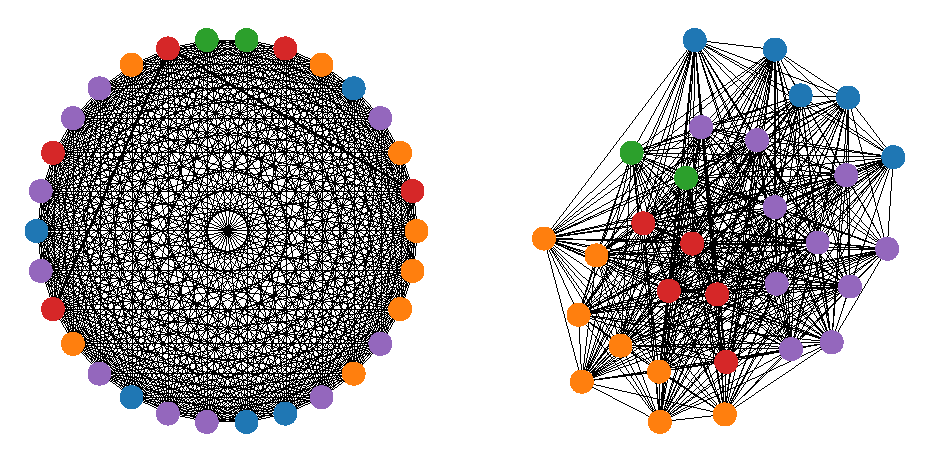
\includegraphics[width=0.40\textwidth]{dose_clustering_figures/graph.pdf}
%	\includegraphics[width=0.59\textwidth]{dose_clustering_figures/graph_bis.pdf}
%	\subfloat[\label{fig:graph-circular} (Circular Layout)]{\hspace{.5\linewidth}}
%	\subfloat[\label{fig:graph-spring} (Spring Layout)]{\hspace{.5\linewidth}}
%	\caption{
%		Plot of the Network\\
%		edges width $\propto$ edge weight $\propto$ $\nicefrac{\text{1}}{\text{distance}}$\\
%		node's color reflects community attribution
%	}
%	\label{fig:graph}
%\end{figure}

%In order to obtain a more precise understanding of the edge weights in the network, one can refer to the adjacency matrix of the edge weights, as depicted in Figure \ref{fig:adjacency}.
%\begin{figure}
%	\centering
%	\includegraphics[width=0.65\textwidth]{dose_clustering_figures/weight_adjacency_matrix.pdf}
%	\caption{Weight Adjacency Matrix of the Network}
%	\label{fig:adjacency}
%\end{figure}

\paragraph{DVH Plot}
%Figure \ref{fig:dvh} illustrates the Dose-Volume Histograms (DVHs), with the colors of the plots corresponding to the communities identified in the network analysis.
%To ensure clarity and prevent confusion, each structure is presented on a separate plot.
%Notably, our observations align with expectations, as doses assigned to nodes within the same community (indicated by the same color) exhibit nearly overlapping DVHs.
%\begin{figure}
%	\centering
%	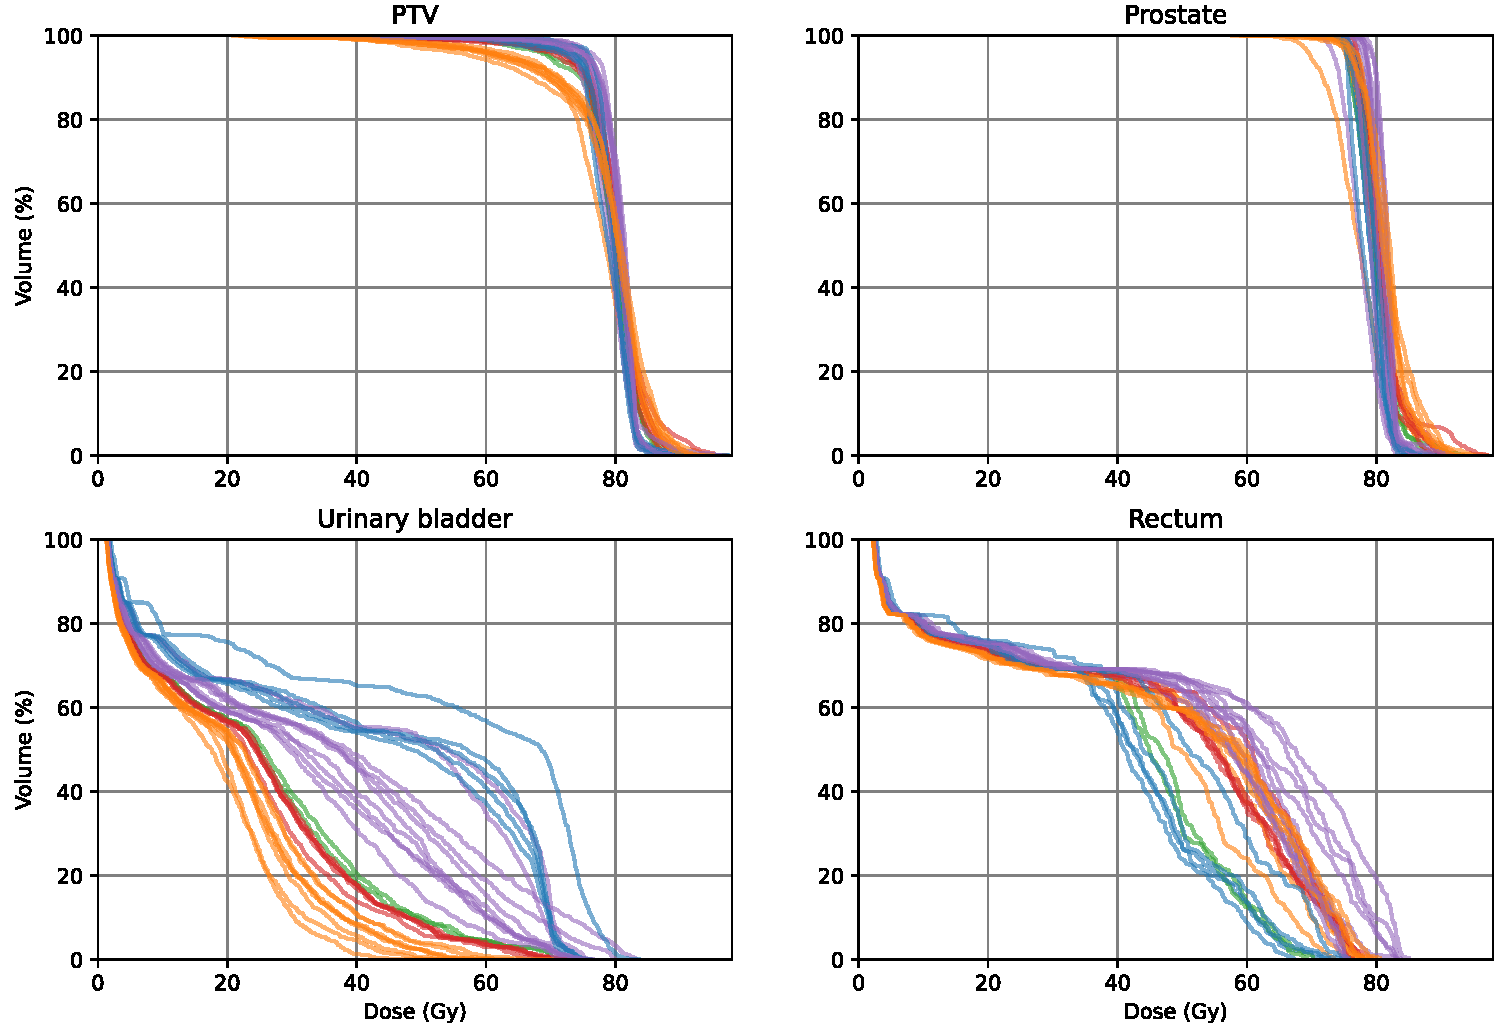
\includegraphics[width=\textwidth]{dose_clustering_figures/dvh.pdf}
%	\caption{Dose-Volume Histogram}
%	\label{fig:dvh}
%\end{figure}

%The visualization of DVHs provides valuable insights into the distribution of doses received by different structures.
%The close correspondence between dose patterns and community assignment underscores the potential of network analysis in uncovering meaningful patterns within radiation therapy data.
%By associating the colors of the DVH plots with the communities identified in the network, we gain a deeper understanding of the relationship between dose assignments and structural characteristics.
%This analysis further supports the notion that nodes (doses) within the same community share similar profiles, suggesting they could be merged, as they will likely have the same clinical effect.

\subsubsection{Dose Clustering Evaluation}
%As explained in \ref{clustering_evaluation}, we use the mean standard deviation of doses at 101 equispaced values of volume to obtain a scalar value of how far apart are a set of doses; see table \ref{table:cluster_std} for results.
%
%\begin{table}
%	\centering
%	\begin{tabular}{|l|c|c|}
%		\hline
%		Set & Set Size & Mean Standard Deviation \\
%		\hline
%		Cluster 1 \textcolor{plt-blue}  {\textbf{(blue)}}   & 4 & 2.0542 \\
%		Cluster 2 \textcolor{plt-orange}{\textbf{(orange)}} & 5 & 0.4049 \\
%		Cluster 3 \textcolor{plt-green} {\textbf{(green)}}  & 2 & 0.3618 \\
%		Cluster 4 \textcolor{plt-red}   {\textbf{(red)}}    & 2 & 0.4218 \\
%		Cluster 5 \textcolor{plt-purple}{\textbf{(purple)}} & 3 & 0.9702 \\
%		Cluster 6 \textcolor{plt-brown} {\textbf{(brown)}}  & 3 & 1.2418 \\
%		\textit{All} & \textit{19} & \textit{3.5122} \\
%		\hline
%	\end{tabular}
%	\caption{Clustering Quality}
%	\label{table:cluster_std}
%\end{table}
%
%The mean standard deviation of the clusters, with values of 2.0542, 0.4049, 0.3618, 0.4218, 0.9702, and 1.2418, averaging at 0.9091, is significantly lower (nearly 4 times lower) compared to the mean standard deviation of the full network, which is 3.5122 (see table \ref{table:cluster_std}).
%This notable reduction in standard deviation yells quantitatively that our clustering approach has favorable results.
%This quantitative assessment is further supported by qualitative results, as illustrated in Figure \ref{fig:dvh}, which demonstrates the meaningfulness and relevance of the dose clusters in characterizing radiation dose distributions.
%Our proposed clustering approach demonstrates strong performance in both qualitative and quantitative evaluations.

\subsection{Discussion}
%The ability to regroup doses into communities provides a valuable insights to understand clinical practices.
%An additional potential application of this technique is the utilization of dose clusters as a similarity measure for early stopping optimization purposes.
%Specifically, if the dose distribution exhibits similarities to the previous $n$ doses, it may serve as an indicator to halt the ongoing optimization process.
%
%However, the clustering of doses is a challenging task, as the dose space is high dimensional and the dose distribution is not smooth.
%The results presented here can not yet be used in clinical practice, they are promising and should be further investigated.

\subsection{Conclusion}
%In conclusion, this study has introduced a novel approach for clustering doses into communities based on their dose distributions, demonstrating the meaningfulness of such clustering both quantitatively and qualitatively.
%This suggests that doses belonging to the same cluster are likely to have indistinguishable clinical effects.
%
%The proposed clustering technique holds several potential applications.
%Firstly, it can be integrated into Fluence Map Optimization (FMO) to facilitate early stopping of the optimization process when the last few updates remain within the same cluster, providing efficiency gains.
%Secondly, if extended to clustering doses from different patients, it could enable the analysis of clinical center practices, offering insights into variations in treatment outcomes among centers for specific anatomies.
%
%Furthermore, this clustering approach has the potential to streamline the validation process between dosimetrists and physicists.
%Currently, multiple treatment plans are submitted for validation, leading to a cumbersome selection process for the physicist.
%However, by clustering the optimized doses with different weight parameters for constraints, the number of options can be reduced, resulting in a more efficient decision-making process and potentially reducing the personnel required in the dosimetry department.
%
%As further research and validation efforts are undertaken, this innovative approach holds considerable promise for enhancing treatment planning processes and, ultimately, improving patient outcomes.



%%%%%%%%%%%%%%%%%%%%%%%%%%%%%%%%%%%%%%%%%%%%%%%%%%%%%%%%%%%%%%%%%%%%%%%%
%                                                                      %
%   %%%%%%%%%%%%%%%%%%%%%%%%%%%%%%%%%%%%%%%%%%%%%%%%%%%%%%%%%%%%%%%%   %
%   %%%%%%%%%%%%%%%%%%%%%%%%%%%%%%%%%%%%%%%%%%%%%%%%%%%%%%%%%%%%%%%%   %
%   %%%%%%%%%%%%%%%%%%%%%%%%%%%%%%%%%%%%%%%%%%%%%%%%%%%%%%%%%%%%%%%%   %
%   %%%%%%%%%%%%%%%%%%%%%%%%%%%%%%%%%%%%%%%%%%%%%%%%%%%%%%%%%%%%%%%%   %
%                                                                      %
%%%%%%%%%%%%%%%%%%%%%%%%%%%%%%%%%%%%%%%%%%%%%%%%%%%%%%%%%%%%%%%%%%%%%%%%


\section[Novel Dosimetry Automation Approach with Graph Theory]{A Novel Framework for Multi-Objective Optimization and Robust Plan Selection Using Graph Theory (ESTRO 2024)}
% many-clicks to few-clicks solution, but goal is one-click
% N-clicks to 2/3-clicks solution, but goal is 1-click

% Poster:
% https://github.com/pauldubois98/ESTRO2024/blob/main/poster-dose_clustering.pdf
% Abstract:
% https://docs.google.com/document/d/1c5GWgAm6TgaTgsQqJVnz9GaSjIlCgfAideT8Rsz4frM/edit?usp=sharing

	
	\chapter{Classical Dosimetry Automation}
	\begin{chapterabstract}
		\lipsum[1-2]
	\end{chapterabstract}
	\clearpage
	\localtableofcontents
	\section{Meta Optimization Approach}

After the FMO step is developed and encapsulated, one may simply modify the weights used for the FMO iteratively, until a condition is met, or for a given number of steps.
We will therefore have one inner optimization (the FMO), and one outer optimization.
\begin{center}
	\begin{minipage}{.55\linewidth}
		\begin{algorithm}[H]
			\caption{Meta Optimization Algorithm Outline}
			\label{alg:meta_optim}
			\begin{algorithmic}
				\State initialize $w$
				\Repeat
					\State initialize $b$ \Comment{FMO starts}
					\Repeat
							\State \textcolor{Prune}{ $d = Lb$ \Comment{differentiable} }
							\State \textcolor{Prune}{ $c = \mathcal{C}(w, d)$ \Comment{differentiable} }
							\State \textcolor{Prune}{ back-propagate $c$ }
							\State \textcolor{Prune}{ update $b$ }
						\Until{\textit{FMO \textbf{stop condition}}} \Comment{FMO ends}
					\State update $w$
				\Until{\textit{Meta-optimization \textbf{stop condition}}}
			\end{algorithmic}
		\end{algorithm}
	\end{minipage}
\end{center}
The outer optimization step is not differentiable (or at least, not in a reasonable computation time).
Hence, we will be looking at gradient-free optimization methods.

\subsection{Expert Weight Adjustment}
Expert systems are computer systems emulating the decision-making of a human expert.

\paragraph{Simple Weight Increase}
One approach is to increase the weight of all constraints that are not met after each FMO optimization.
\begin{itemize}
	\item \textbf{Advantages:} Very simple to implement, and understand.
	\item \textbf{Disadvantages:} If none of the constraints is met, then the outer loop is stuck.
	This method might struggle to converge in complex cases where multiple constraints compete.
\end{itemize}

\paragraph{Inverse Proportional Weight Increase}
Another approach is to increase the weight of each constraint inversely proportional to how close it is to being met, quantifying the degree to which a constraint is satisfied.

Quantification Example: use the area bounded by the DVH constraint, and the DVH curve.
When this is zero, then the constraint is met.
\begin{itemize}
	\item \textbf{Advantages:} Still relatively easy to implement, and allows for a more nuanced adjustment of weights based on constraint satisfaction.
	\item \textbf{Disadvantages:} This method can lead to an oscillation phenomenon, where constraints fluctuate between satisfaction and violation.
\end{itemize}
Of course, 	one could add momentum to smooth the process, to fix the oscillation problem.
However, expert systems like these often require constant refinement, hence, this path is not viable for a credible clinical application.

\subsection{Metric-Based}
Here, we suppose that one can construct a measure of the quality of a plan.

\paragraph{Hill Climbing}
Hill climbing is a simple optimization technique where the solution iteratively moves towards a better solution based on a defined metric.

In our context, several metrics have been proposed to quantify the quality of a radiotherapy treatment plan, such as Normal Tissue Complication Probabilities (NTCP), target coverage, conformity index, and heterogeneity index, among others \cite{lyman_normal_1992,li_input_2022}\label{metrics}.
\begin{itemize}
	\item \textbf{Advantages:} Provides a systematic way to improve plans.
	\item \textbf{Disadvantages:} Defining the correct metric of interest is hard.
\end{itemize}
However, none of these metrics alone nor in combination with others has proven to satisfy radio-oncologists.
In practice, the most reliable way to assess a treatment plan is by manually evaluating the dose-volume histograms (DVHs), which provide a detailed look at the dose distribution across both the target and the organs at risk.

% Full paper:
% https://github.com/pauldubois98/AIME2024/blob/main/llncs_formatting.pdf
\section{Radiotherapy Dose Optimization via Clinical Knowledge Based Reinforcement Learning (AIME 2024)}
\paragraph{Abstract}
%% Achieving optimal dose distribution in radiation therapy planning is a complex task, with contradicting goals. Yet, this step is crucial with profound implications for patient treatment.
%% The absence of universally agreed-upon constraints prioritization in radiation therapy planning complicates the definition of an optimal plan, requiring a delicate balance between multiple objectives. This balance usually ends up being done manually.
%A radiation therapy plan finds an equilibrium between goals with no universal prioritization. The delicate balance between multiple objectives is typically done manually.
%The optimization process is further hindered by complex mathematical aspects, involving non-convex multi-objective inverse problems with a vast solution space.
%Expert bias introduces variability in clinical practice, as the preferences of radiation oncologists and medical physicists shape treatment planning.
%
%To surmount these challenges, we propose a first step towards a fully automated approach, using an innovative deep-learning framework.
%Using a clinically meaningful distance between doses, we trained a reinforcement learning agent to mimic a set of plans.
%This method allows automatic navigation toward acceptable solutions via the exploitation of optimal dose distributions found by human planners on previously treated patients.
%As this is ongoing research, we generated synthetic phantom patients and associated realistic clinical doses.
%Our deep learning agent successfully learned correct actions leading to treatment plans similar to past cases ones.
%The incapacity to reproduce human-like dose plans hinders adopting a fully automated treatment planning system; this method could start paving the way towards human-less treatment planning system technologies. % "tie conclusion of reasoning why we do this technique."
%In future work, we hope to be able to apply this technique to real cases.

\subsection{Introduction}
%In contemporary radiation therapy, photon intensity modulated radiation therapy (IMRT) is a pivotal technique to attain precise and conformal dose distributions within target volumes \cite{xu_comparison_2017}.
%This achievement owes its realization to the advent of the multileaf collimator (MLC) \cite{galvin_characterization_1993}.
%Radiation therapy is now a reliable treatment for oncology \cite{valentini_survival_2009}.
%Despite this consensus, the way to deliver radiotherapy for its best result remains very dependent upon doctors.
%Moreover, there appears to be a large variability across physicians and centres, but in terms of 3D structures contouring and irradiation, constrains priorities \cite{variability_2021}.
%
%To achieve the best treatment, doctors must solve a complex inverse mathematical optimization problem with multiple trade-offs \cite{oelfke_inverse_2001} \cite{webb_physical_2003}.
%However, a lack of standardized prioritization of constraints makes the optimization a real challenge.
%The standard procedure nowadays is to guide computer optimization manually: dosimetrists manually update the settings of an optimizing software so-called Treatment Planning System (TPS) \cite{planification_website}.
%
%There have been many tries to create a metric that quantifies the quality of a treatment plan, such as Normal Tissue Complication Probabilities (NTCP), target coverage, conformity index, and heterogeneity index, among others/to name a few \cite{lyman_normal_1992} \cite{li_input_2022}\label{metrics}.
%However, they have yet to satisfy all radio-oncologists, and the only reliable way to assess a doctor's plan is to evaluate the dose-volume histograms (DVHs) themselves.
%
%As a result, Pareto surface exploration is unsuitable due to the lack of impartial quantitative measurement for a particular plan \cite{huang_pareto_2021}.
%Other meta-optimization techniques are similarly bounded for the same reason \cite{wu_optimization_2001} \cite{xing_optimization_1999}.
%An extra challenge to attend for those is the fact that not all cases have the same difficulty.
%Hence, for an "easy" case, doctors will require an excellent dose (in terms of the metrics mentioned above), while they can be more permissive for "harder" cases.
%The context-aware acceptability criteria make the acceptability of a plan hard to define in general.
%
%Reinforcement learning (RL) is a machine learning paradigm that trains agents to make sequential decisions in dynamic environments \cite{brooks_what_2021}.
%Agents learn to optimize their actions to achieve long-term objectives through trial and error guided by rewards or penalties.
%The decisions taken by dosimetrists when optimizing treatment can be formalized as an RL problem.
%Moreover, dosimetrists can guide the TPS towards an acceptable plan but usually struggle to explain their decision while interacting with the TPS.
%The difficulty in explaining why certain decisions are taken suggests using deep RL over expert-based methods.
%This setup is similar to image recognition, where one can say a picture represents a car or a boat but struggles to explain why.
%
%The study’s primary hypothesis is that all the information needed to decide what weights should be changed in the objective function used by the optimizer relies on the Dose Volume Histograms (DVHs).
%Our hypothesis is supported by the fact that dosimetrists almost solely use DVHs plots.
%In order to learn the actions of dosimetrists who use a TPS to optimize doses, we leverage deep learning.
%This is done by training an agent that takes the DVHs as the input of the current optimized dose, and predicts the evaluation of possible weights changes.
%
%Typically, access to the exact actions taken by human dosimetrists on the TPS is unavailable (as clinics do not usually store this data; only the final plan is held).
%Therefore, we only use the dose distributions of previously treated patients to train our model.
%This partial availability of data suggests the use of RL.

\subsection{Materials and Methods}
%We introduce a new paradigm for reward-based dosimetrist RL agents.
%This new reward system aims to improve how human-optimized doses are mimicked.

\subsubsection{Reinforcement Learning Reward}

%\begin{figure*}
%	\centering
%	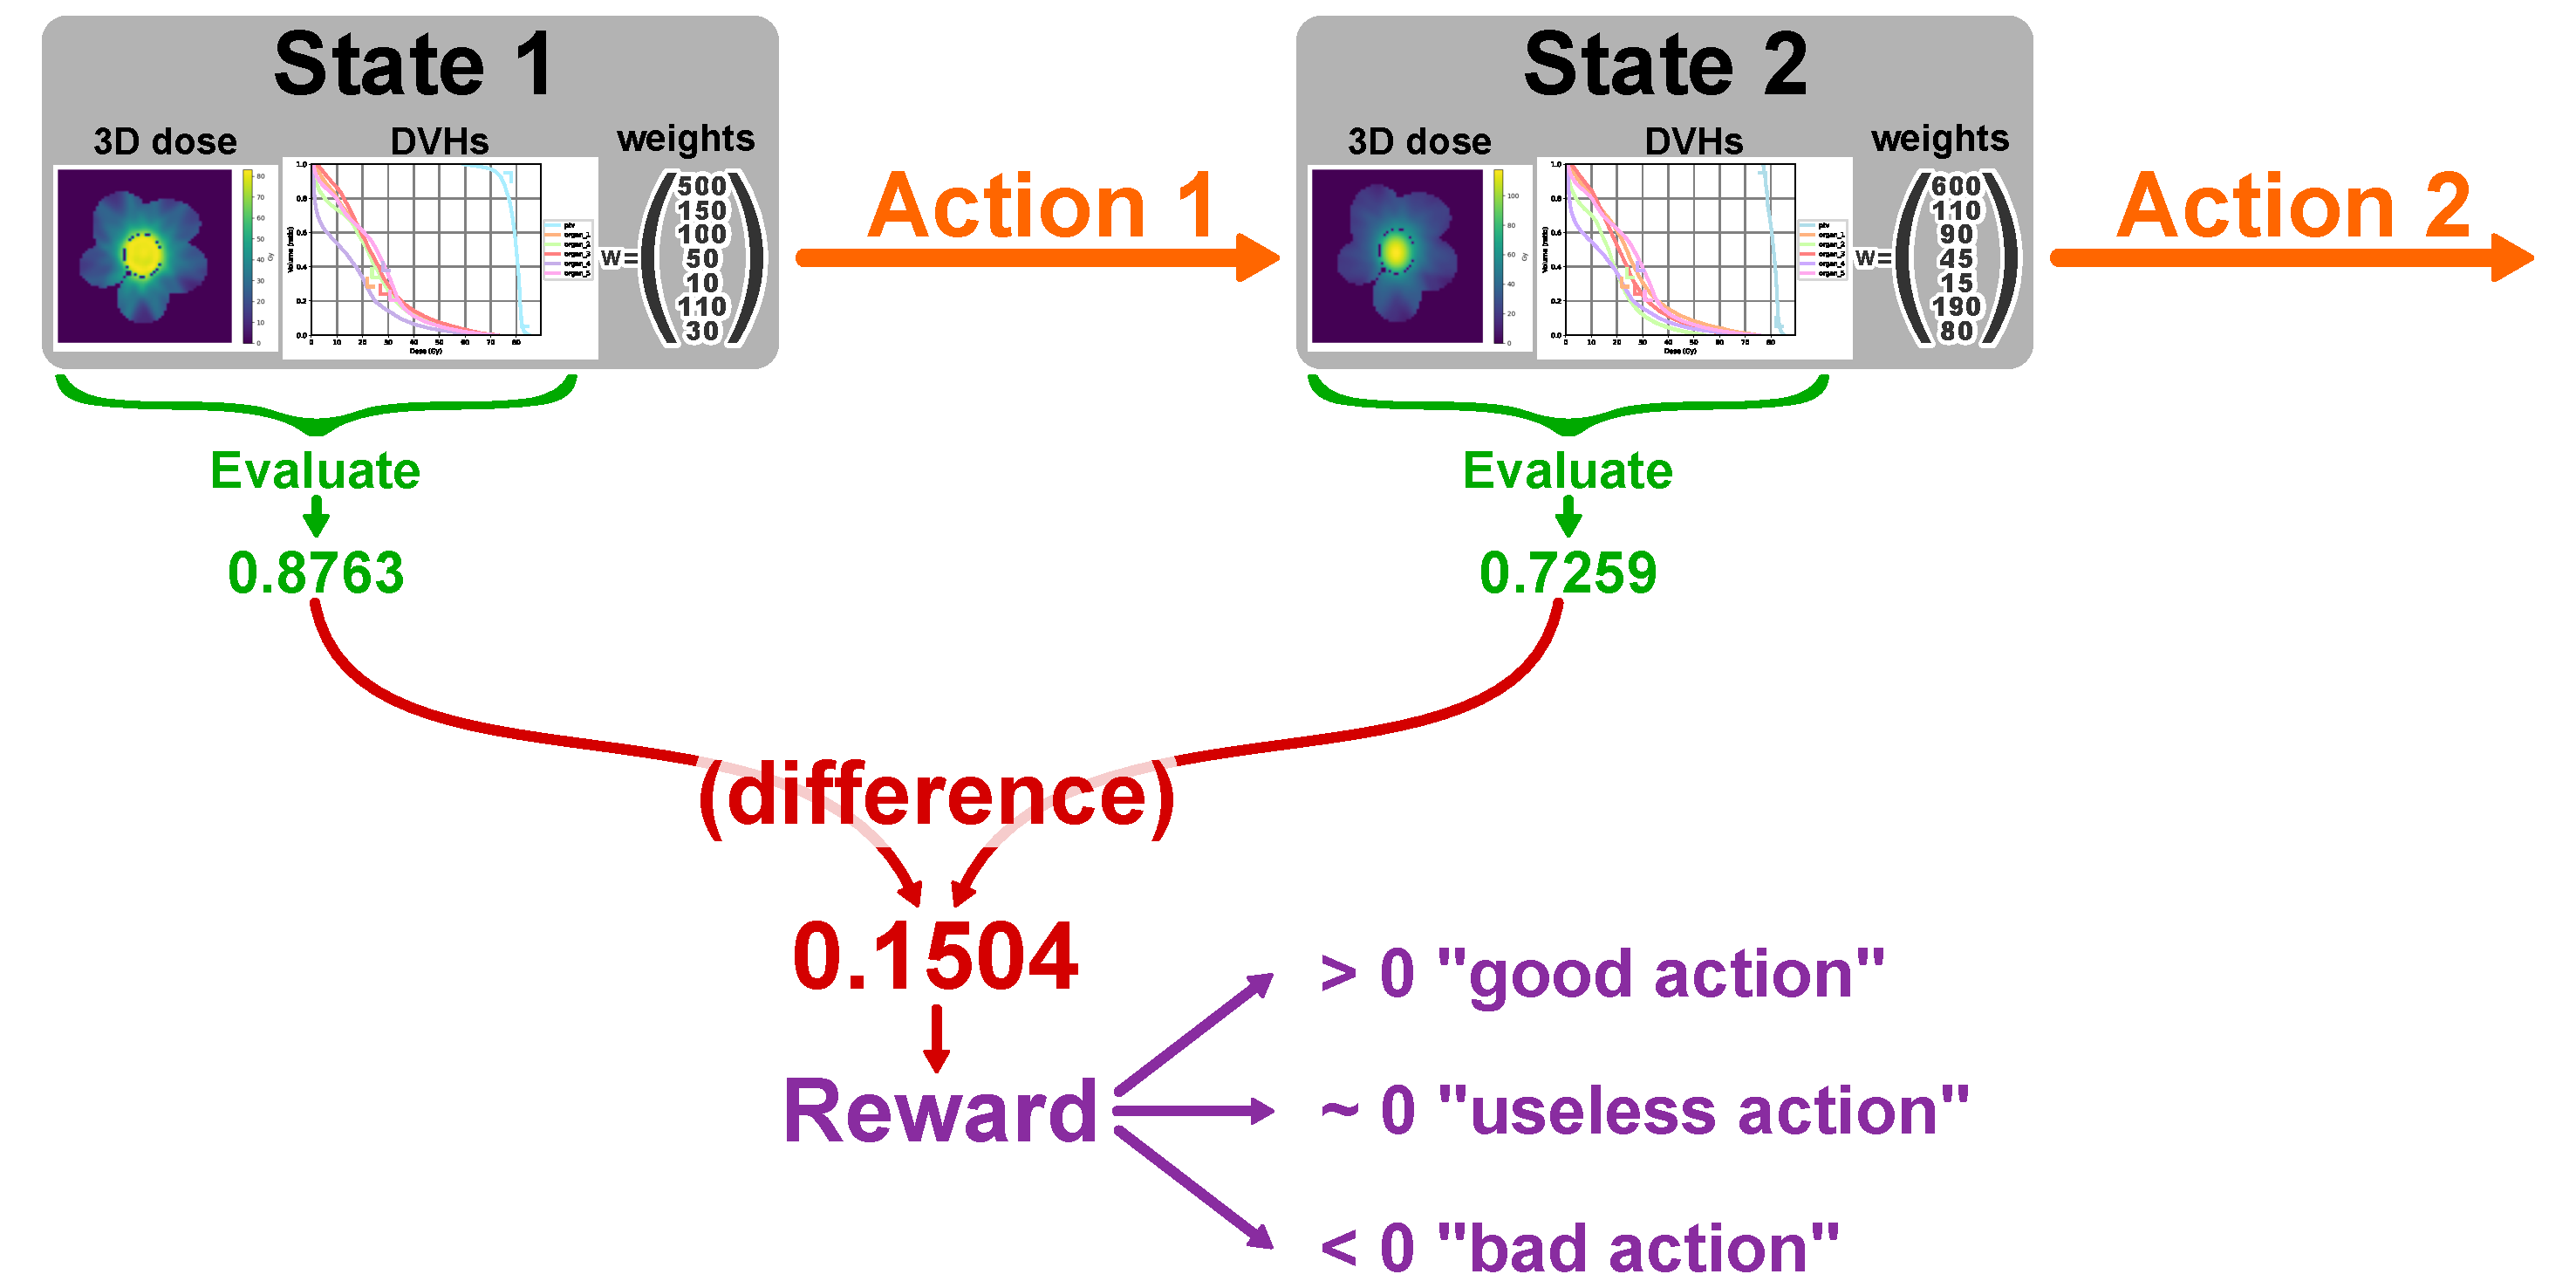
\includegraphics[width=0.9\textwidth]{AIME/reward.pdf}
%	\caption{Classical reinforcement learning reward for automatic dosimetry.}
%	\label{fig:reward_fig}
%\end{figure*}
%
%In classical RL, we want $V(S_t) = R_t + \gamma V(S_{t+1})$
%(so the update is $V(S_t) \leftarrow (1-\alpha) V(S_t) + \alpha \left[ R_{t+1} + \gamma V(S_{t+1}) \right]$).
%In the context of dose optimization, the reward $R_t$ is defined as $R_t = \mathcal{E}(S_{t+1}) - \mathcal{E}(S_t)$, where $\mathcal{E}$ is a function that evaluates the quality of a state (such that higher is better; if lower is better, then swap $s_t$ and $S_{t+1}$).
%
%The evaluation $\mathcal{E}$ can be one or a mixture of the metrics mentioned in the introduction (Section \ref{metrics}) \cite{shen_hierarchical_2021} \cite{shen_intelligent_2019} \cite{moreau_reinforcement_2021}.
%This setup may leverage knowledge about which actions to perform instead of guessing randomly, as a meta-optimizer would do.
%This could potentially gain some computation time.
%
%However, this technique does not use past plans; it only needs the optimizer inputs (CT, structures contours).
%We propose using the availability of past treatment plans to more accurately reflect the complexity of decisions made by dosimetrists and better match their expectations of a fully automatic treatment planning system.
%
%As developed in previous work, we can derive a distance between dose plans \cite{paul_dubois_novel_2024}.
%If we consider the clinical dose of past cases (used for training) as the best achievable one, we can evaluate a dose plan by computing its distance from the clinical dose plan.
%
%Let $D_t$ be the dose associated with $S_t$, and $D_C$ the clinical dose.
%We then define $\mathcal{E}(S_t) = \mathcal{D}(D_t, D_C)$.
%Since, in that case, $\mathcal{E}(S_t)$ should be minimized, we will define the reward as $$R_t = \mathcal{E}(S_t) - \mathcal{E}(S_{t+1}) = \mathcal{D}(D_t, D_C) - \mathcal{D}(D_{t+1}, D_C).$$
%This reward can be interpreted as the "distance gained to the clinical dose". 

\subsubsection{Architecture}
%We use a dense neural network, which inputs the DVHs and current normalized weight values.
%It outputs the $Q(s, a)$ value for each possible action $a$.
%Dense layers are very prone to overfitting.
%In order to force the network to actually predict the following evaluation for each possible action, without overfitting, we incorporated a bottleneck in the network (Figure \ref{fig:architecture}).
%Compressing the information stops the network from overfitting.
%Networks with such architecture show very little difference between training and validation sets (see Figure \ref{fig:losses_training}).
%
%\begin{figure*}
%	\centering
%	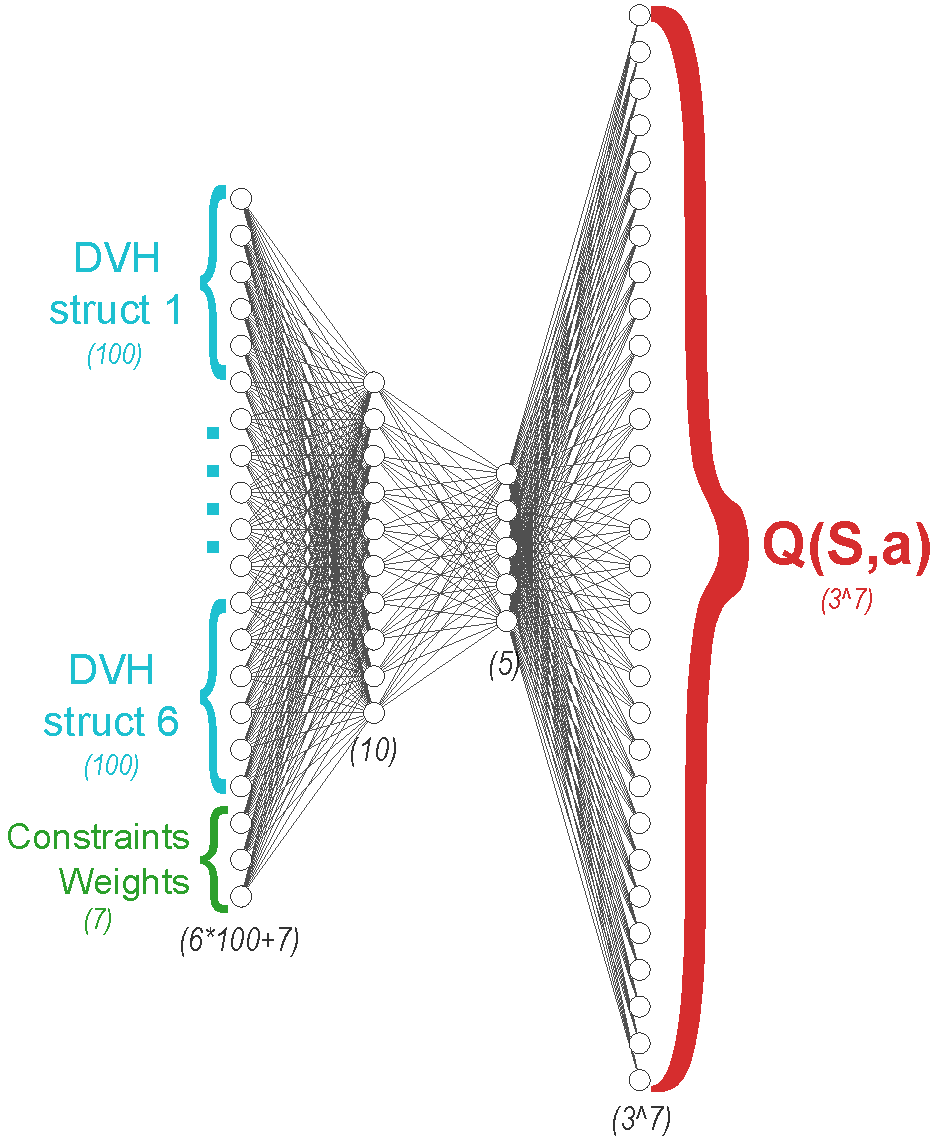
\includegraphics[width=5cm]{AIME/architecture_all_actions.pdf}
%	\hspace{0.5cm}
%	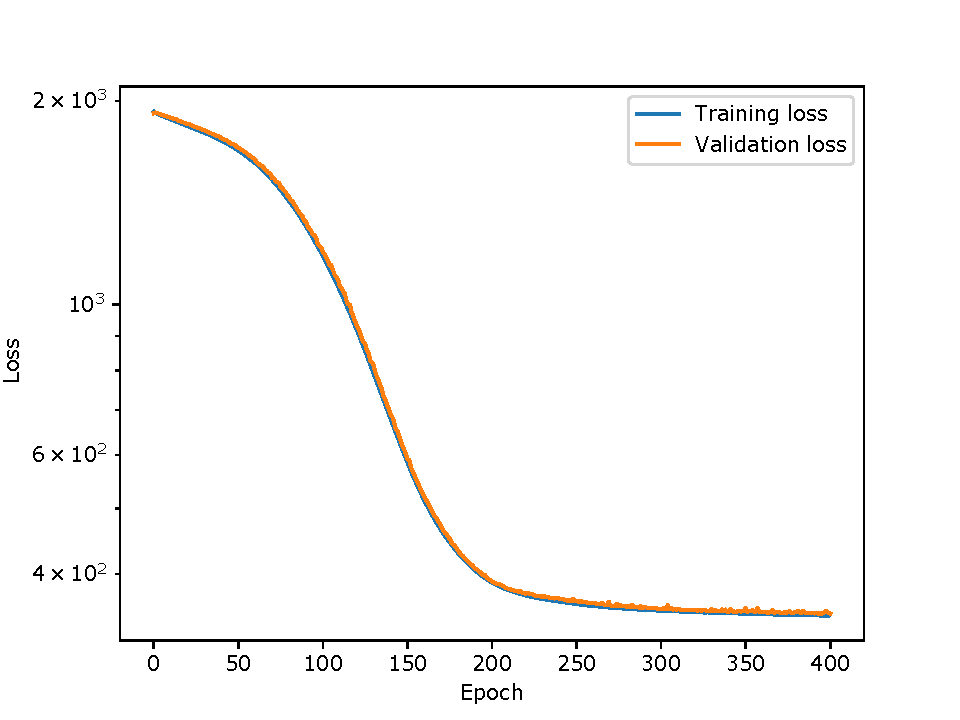
\includegraphics[width=6cm]{AIME/losses-distance.pdf}
%	\caption{Neural network architecture and loss evolution while training.}
%	\label{fig:architecture}
%	\label{fig:losses_training}
%\end{figure*}

\subsubsection{Avoiding Off-Distribution}
%We generated a training set of over 125k actions (this took five days on an NVIDIA GeForce GTX 1080).
%Despite this relatively large dataset, we have not explored exhaustively the state-actions space, and the network still lands off-distribution.
%This can easily be spotted when the predicted $Q$ value is greater than the current distance to the clinical dose; we choose to ignore those predictions, and in fact all outlier predictions.
%The justification is that our set of actions is limited, no action will suddenly drastically improve the plan.
%It is the combination of several sequential actions that allows good plan optimization.
%Therefore, while testing, we choose the action with the best prediction, while passing the outlier test just mentioned.
%
%\subsection{Results}
%Figure \ref{fig:distance} shows how the distance between our RL agents performs over five steps on 30 test patients (unseen during the training).
%A lower distance is interpreted as an improved dose, since it is closer to the best dose, which is the clinical one.
%\begin{figure*}
%	\centering
%	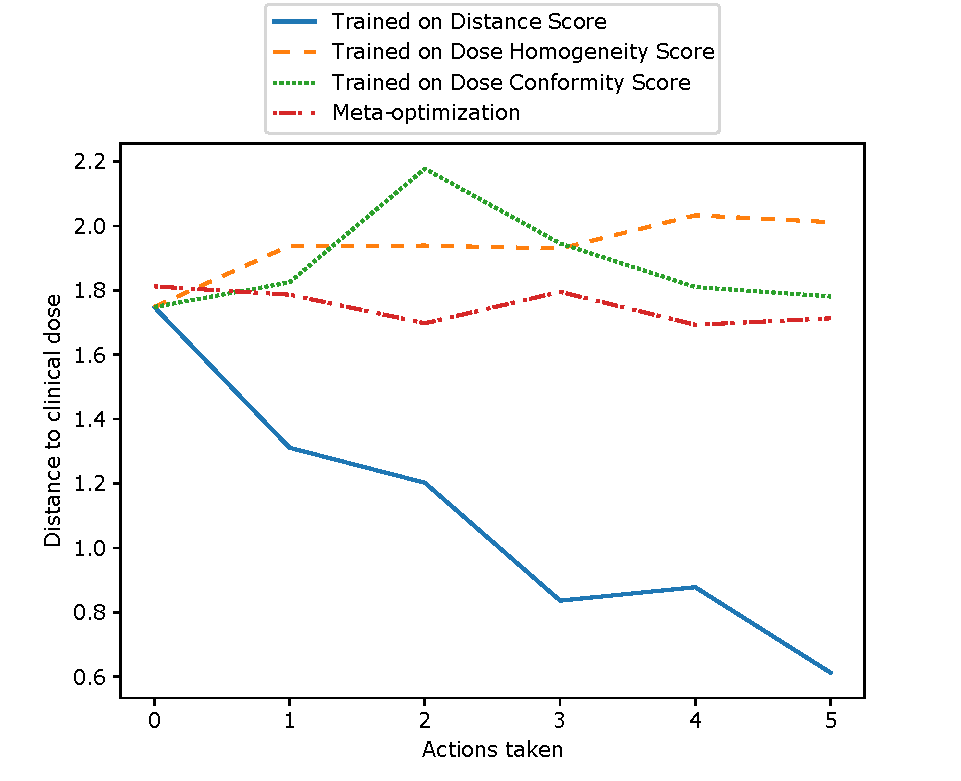
\includegraphics[width=0.6\textwidth]{AIME/DistanceToClinicalDose.pdf}
%	\caption{Average distance between RL agent's dose and clinical dose.}
%	\label{fig:distance}
%\end{figure*}


\subsubsection{Quantitative Results}
%The network converged on the training data, and validation showed minor overfitting.
%For testing, we generated 30 brand new cases that we again manually optimized.
%We then used the RL model to perform the optimization of these 30 unseen cases.
%On average, our model was able to reduce the dose distance with manually optimized dose by a factor of $~3$ (from $~1.8$ at iteration $0$ to $~0.6$ at iteration $4$), as shown in Table \ref{table:results}.
%
%We remark from the Table \ref{table:results} that the homogeneity score and conformity score give similar results.
%Classical meta-optimization performs well, but needs a metric to elect the best dose (during the test, the clinical dose is unknown, so the DVHs distance metric is not available).
%We also observe that clinical doses are not always scoring high (in this test set, a high conformity, but low homogeneity compared to automatic techniques).
%This show the difficulty to create a metric that capture all the complexity of a clinically acceptable dose.
%
%\begin{table}
%	\begin{center}
%		\begin{tabular}{| c || c | c | c |} 
%			\hline
%			Agent $\backslash$ Metric & Mean Final Distance$^*$ & Homogeneity Score$^\dagger$ & Conformity Score$^\dagger$ \\ 
%			\hline
%			RL Distance Score & \textbf{0.612} & 1.871 & 0.406 \\ 
%			RL Homogeneity Score & 2.012 & \textbf{4.387} & 0.567 \\
%			RL Conformity Score &  1.770  & 4.017 & 0.507 \\
%			Meta-optimization & N/A & 4.117 & \textbf{0.610} \\
%			\textit{Clinical doses} & \textit{0} & \textit{1.541} & \textit{0.580} \\	
%			\hline
%		\end{tabular}
%		\label{table:results}
%	\end{center}
%	\caption{
%		Average performances of four algorithms tested on DVHs distance to clinical dose, dose homogeneity-based score, and conformity-based score.\\
%		\textit{$^*$: distance is imporved performance through a lower score.} \\
%		\textit{$^\dagger$: score is imporved performance through a higher score.}
%	}
%\end{table}
%\vspace{-1.4cm}

\subsubsection{Qualitative Results}
%Figure \ref{fig:steps} shows the DVHs at each of the first four optimization steps on one of the test patients, unseen by the agent during the training.
%Our model drastically reduced the dose distance with manually optimized doses.
%Visual inspection of the DVHs plot shows that the dose optimized by the RL agent is very close to the clinical (manually fine-tuned) one.
%
%\begin{figure*}
%	\centering
%	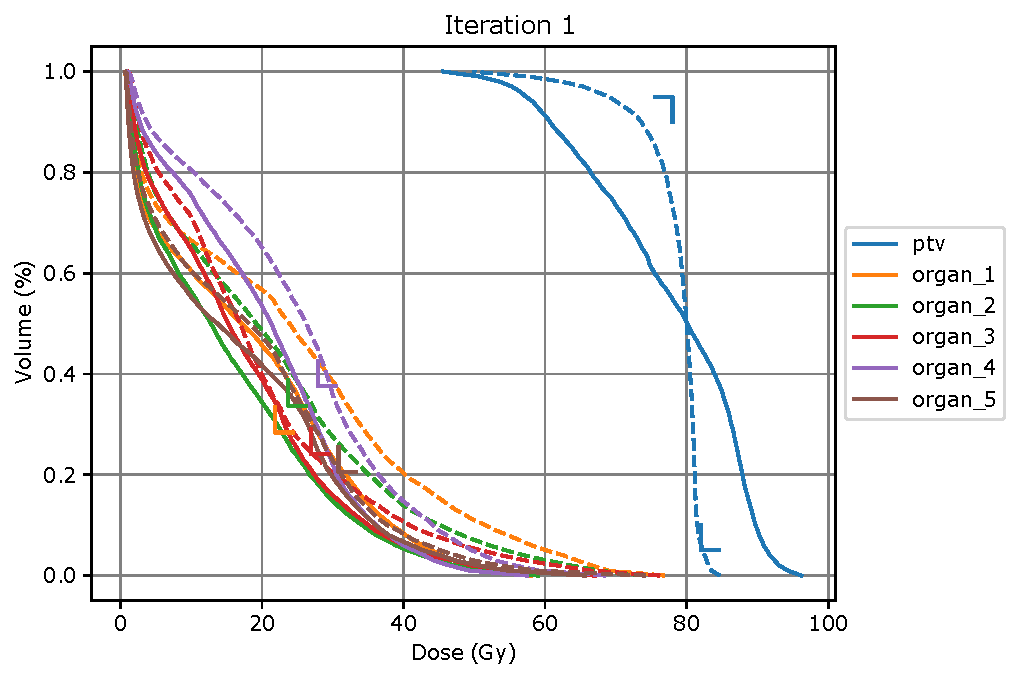
\includegraphics[width=0.49\textwidth]{AIME/distance-test-w1.pdf}	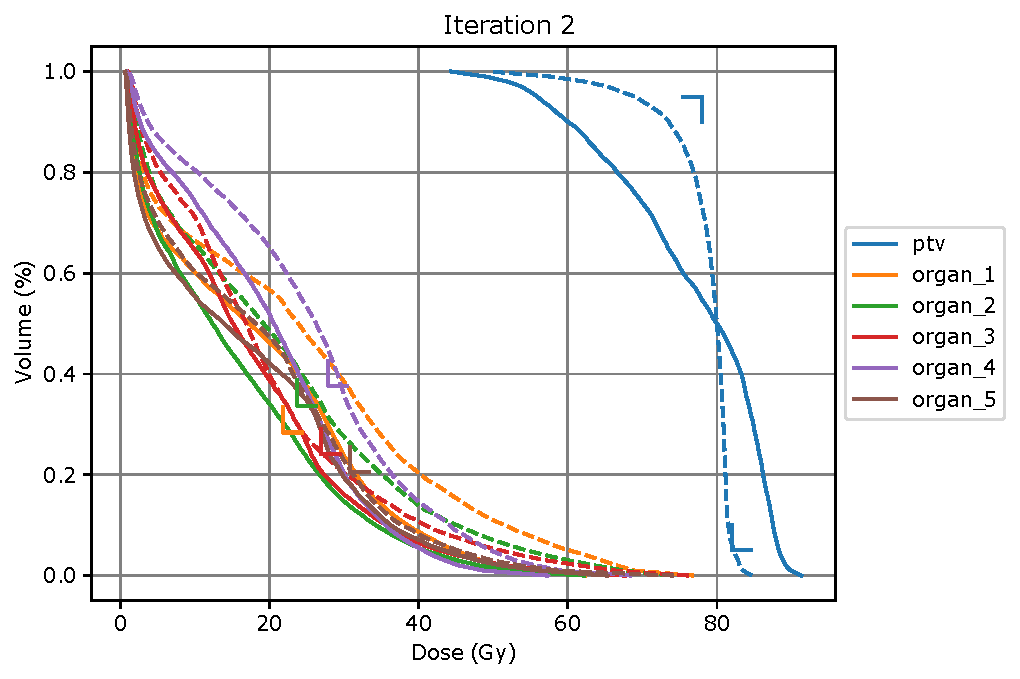
\includegraphics[width=0.49\textwidth]{AIME/distance-test-w2.pdf}	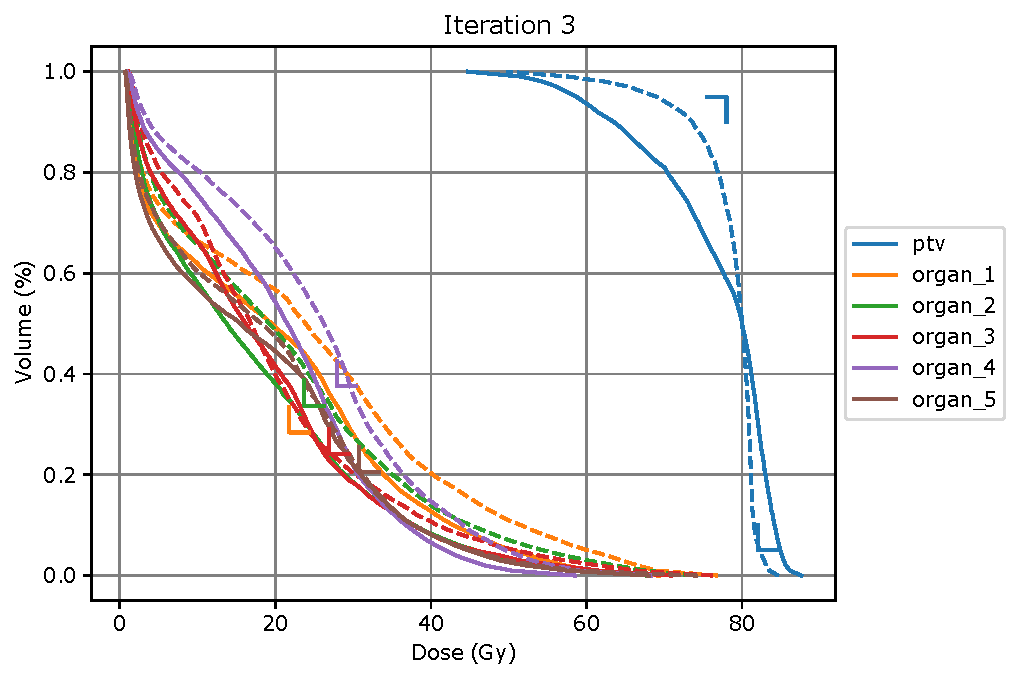
\includegraphics[width=0.49\textwidth]{AIME/distance-test-w3.pdf}	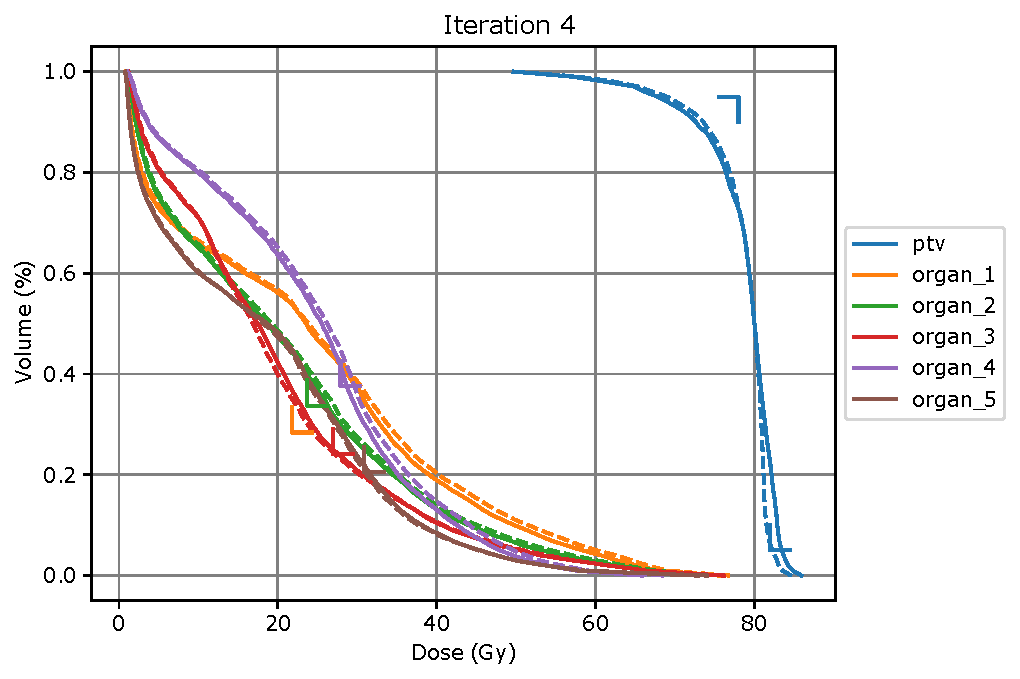
\includegraphics[width=0.49\textwidth]{AIME/distance-test-w4.pdf}
%	\caption{RL Agent DVHs after each action taken on a test (unseen) patient. Solid lines are the agent's dose DVHs; dotted ones are the reference dose DVHs (manually fine-tuned).}
%	\label{fig:steps}
%\end{figure*}

\subsection{Discussion}
%Our study demonstrates the potential of deep RL for automating radiotherapy treatment plan optimization.
%A key strength of our approach is its ability to learn from past treatment plans, capturing the complex decision-making processes of human dosimetrists.
%This data-driven approach avoids the limitations of pre-defined metrics, which may not fully capture the nuances of optimal treatment planning.
%
%However, our study also has limitations.
%The agent's performance relies on the quality and quantity of available training data.
%Cases with limited historical data or complex anatomical features may require additional strategies.
%Moreover, while the agent achieves promising results regarding dose distance reduction, the dose is not guaranteed to be clinically acceptable.
%Although this study demonstrates the promise of our RL approach in a controlled setting, one final limitation to mention is that extending it to real-world radiotherapy planning would necessitates addressing additional complexities and constraints.
%
%Several avenues exist for further research.
%Firstly, we plan to investigate strategies for incorporating additional information, such as patient characteristics and anatomical complexities, into the training process.
%Secondly, we aim to explore techniques for improving the interpretability of the agent's decision-making process, allowing for better understanding and potential clinical validation.

\subsection{Conclusion}
%Our approach differs from previous RL-based methods for radiotherapy planning in two key aspects.
%First, we avoid relying on pre-defined metrics for evaluation, which can be subjective, and limit the agent's ability to learn complex optimization strategies.
%Second, compared to traditional meta-optimization approaches, our method leverages past treatment data, potentially leading to more informed decision-making during the optimization process.
%
%This study demonstrates deep RL's feasibility and potential benefits for automating radiotherapy treatment plan optimization.
%Our approach is capable of directly predicts state evaluations, and shows promise in achieving significant improvements in efficiency and, potentially, treatment outcomes.
%Further research is needed to address limitations, improve interpretability, and ensure safe clinical integration.
%This approach could revolutionize radiotherapy planning, leading to more standardized, efficient, and improved patient care.

\subsection*{Appendix}
%As this is very new and ongoing research, we generated synthetic phantom patients and associated trustable clinical doses.
%In future work, we hope to apply this technique to real cases.

\subsubsection*{Synthetic phantom patients}
%We generated 130 patients with oval axial section bodies.
%We set the body density to water density.
%We then added an ellipsoid PTV within the body, with a slightly different density (following $\mathcal{N}(1,0.05)$).
%Likewise, we generate five organs gravitating around the PTV, aligned on the axial section.
%
%\begin{figure*}
%	\centering
%	\label{fig:main_slice-ct}
%	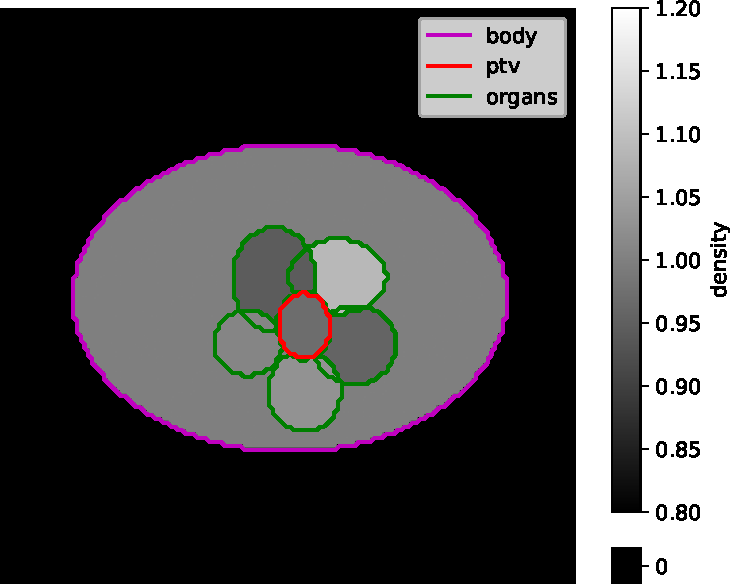
\includegraphics[height=3.5cm]{AIME/main_slice-ct.pdf}
%	\hspace{0.5cm}
%	\label{fig:main_slice-dose}
%	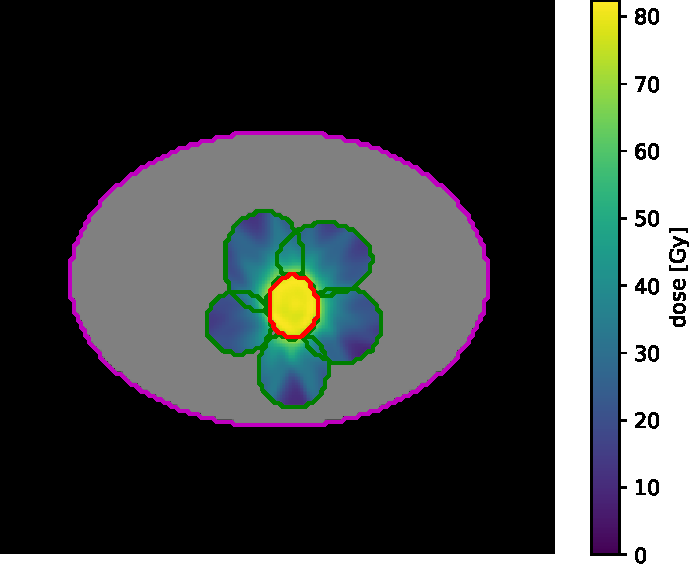
\includegraphics[height=3.5cm]{AIME/main_slice-dose.pdf}
%	%	\hspace{0.1cm}
%	\\
%	\label{fig:clinical_dvh}
%	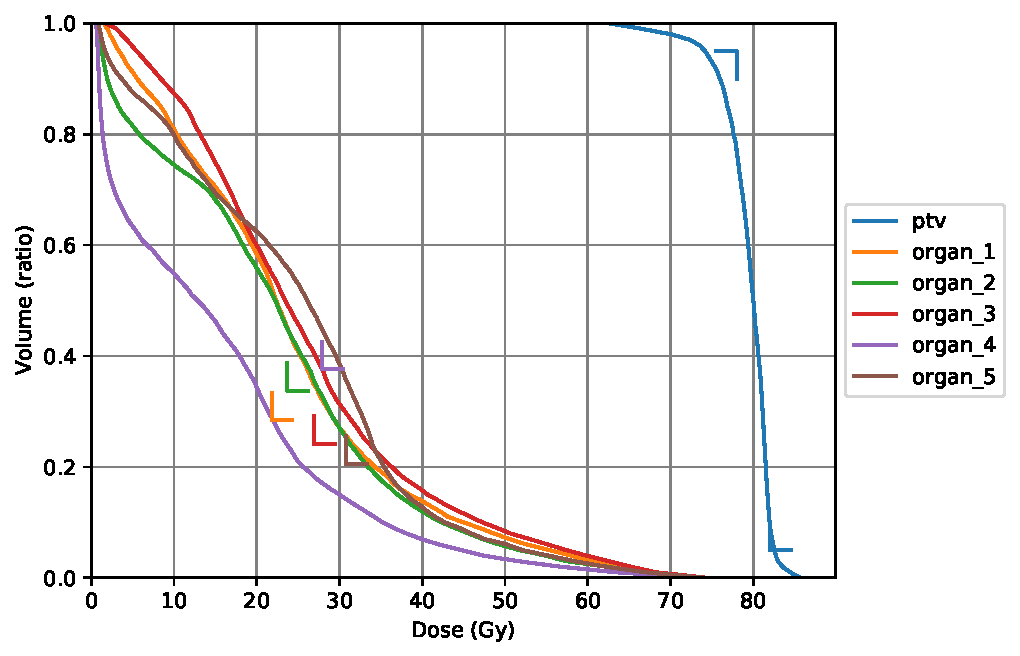
\includegraphics[width=7cm]{AIME/dvh_example.pdf}
%	\caption{
%		Example of a (generated) patient: \\
%		\textit{Left:} Main axial slice (center of the PTV) \textbf{CT}.\\
%		\textit{Right:} Main axial slice (center of the PTV) of the \textbf{clinical dose}. \\
%		\textit{Bottom:} Associated clinical dose \textbf{DVH}.
%	}
%	
%\end{figure*}
%\vspace{-1cm}

\subsubsection*{Clinical dose}
%After generating the patient's CT and structures, we needed to create a reference dose that our agent should mimic.
%We manually set weights and performed a standard optimization.
%The dose prescription is a standard 80Gy on PTV, the same across all patients.
%We used a seven-beam IMRT irradiation technique on all the cohorts.


\subsubsection*{Optimization}
%We optimize the plan using the LBFGS optimizer (shown to be the most appropriate in \cite{dubois_radiotherapy_2023}).
%For each DVH constraint (e.g. for PTV, $D_{95}>80 \ Gy$), we used a linear penalization of the overdose.



%%%%%%%%%%%%%%%%%%%%%%%%%%%%%%%%%%%%%%%%%%%%%%%%%%%%%%%%%%%%%%%%%%%%%%%%
%                                                                      %
%   %%%%%%%%%%%%%%%%%%%%%%%%%%%%%%%%%%%%%%%%%%%%%%%%%%%%%%%%%%%%%%%%   %
%   %%%%%%%%%%%%%%%%%%%%%%%%%%%%%%%%%%%%%%%%%%%%%%%%%%%%%%%%%%%%%%%%   %
%   %%%%%%%%%%%%%%%%%%%%%%%%%%%%%%%%%%%%%%%%%%%%%%%%%%%%%%%%%%%%%%%%   %
%   %%%%%%%%%%%%%%%%%%%%%%%%%%%%%%%%%%%%%%%%%%%%%%%%%%%%%%%%%%%%%%%%   %
%                                                                      %
%%%%%%%%%%%%%%%%%%%%%%%%%%%%%%%%%%%%%%%%%%%%%%%%%%%%%%%%%%%%%%%%%%%%%%%%



% Full abstract:
% https://github.com/pauldubois98/ASTRO2024/blob/main/abstract.pdf
\section{Clinically Dependent Fully Automatic Treatment Planning System (ASTRO 2024)}
\subsection{Purpose / Objective}
%Although fully automated treatment planning system (TPS) has several advantages, such as the ability to treat more patients and optimize treatments, clinics have not adopted it because there is a wide variation of practices between them.
%Additionally, dosimetrists make complex compromises while manually optimizing with a TPS, which is too complex to be captured by a metric, or not computable in a reasonable time.
%Here, we propose a solution adaptable to each clinic's practices: a reinforcement learning (RL) agent trained to mimic human dosimetrists' optimization on a cohort of previously treated patients.
%We hypothesize that by training one agent for each clinic, we ensure that guidelines specific to each of them are followed.

\subsection{Materials/Methods}
%RL agents adapt actions to situations where there are interactions with an environment.
%RL only needs a reward after performing an action.
%In the case of dose optimization, adjusting the weights of the constraints are the actions.
%The key is to find a way of rewarding the agent when making good decisions (actions) versus bad ones.
%Current RL methods in dosimetry struggle to mimic human-optimized plans.
%We propose a new reward system based on the dose distribution of past clinical cases, via calculating the DVHs differences between the agent dose, and the database dose.
%This would better guide the RL agent towards clinically-acceptable treatment plans.
%Most importantly, it also allows the optimization to fit each center's internal standard practices and guidelines.

\subsection{Results}
%We successfully trained agents to mimic the dose type of several clinics.
%We generated a cohort of 50 patients to train them and manually optimized the dose according to three guidelines.
%We then generated 20 other patients for testing purposes.
%The table shows the average difference between clinical doses and the ones optimized by our RL agents.
%Agents specializing in one type of guideline managed to mimic it, but performed poorly on others.
%Thus, for a clinically helpful, fully-automated TPS, one RL agent should be trained for each clinical guideline.

\subsection{Conclusion}
%By leveraging past clinical dose data, we have demonstrated the feasibility of training RL agents to mimic human-optimized radiotherapy plans following specific clinical guidelines.
%The results show that agents trained on specific clinic guidelines perform better in mimicking those guidelines than a single, general-purpose agent.
%This finding supports our hypothesis that a fully automatic TPS tailored to each clinic's practices is achievable.
%Future work could involve expanding the patient cohort to non-phantom cases, including modalities other than prostate cases, and real-world testing with human oversight to ensure the safety and efficacy of the RL-based TPS.
%Our research could pave the way for developing clinically-dependent automated TPS.

%Table of average DVHs distances on test cases:
%To Clinic A	To Clinic B	To Clinic C
%RL on clinic A	1.6	2.2	5.1
%RL on clinic B	2.3	1.3	2.3
%RL on clinic C	2.7	2.5	1.6

	
	\chapter{Dosimetry Automation via Mimicking}
	\begin{chapterabstract}
		\lipsum[1-2]
	\end{chapterabstract}
	\clearpage
	\localtableofcontents
	% https://github.com/pauldubois98/SFPM-JS2024
\section[DVH Guided Deep Dose]{Dose-Volume Histograms Guided Deep Dose Prediction for Radiotherapy Treatment Planning (SFPM 2024)}
\subsection{Introduction}
Traditionally, the creation of radiotherapy treatment plans has been a semi-manual process, where dosimetrists finetune importance factors assigned to structures and constraints.
A cost function is then used through a classical optimization algorithm to calculate the optimal plan.

In recent years, deep learning in treatment planning has gained attention.
Deep learning models can predict the three-dimensional dose distribution based on patient-specific anatomical data derived from medical imaging (CT scans).
While the predicted dose distribution may not directly represent a deliverable treatment plan, it serves as the basis for determining a clinically viable plan through dose mimicking.
Dose mimicking is an optimization technique that eliminates the need for manual adjustment of importance factors by dosimetrists.
Therefore, the ability to predict a clinically acceptable and near-deliverable 3D dose distribution for any patient presents significant potential for fully automating the radiotherapy planning process.
It is important to note that the successful application of dose mimicking \cite{McIntosh2017,Sun2022} requires a target dose distribution that is nearly deliverable; thus, arbitrarily setting the target dose to zero for OARs is not feasible.

However, this approach requires further adaptation to accommodate specific clinical guidelines.
A potential solution involves training individualized models for each treatment center, allowing institution-specific practices and guidelines to be incorporated.
However, deep learning dose prediction models are computationally large, and implementing separate models for each center is resource-intensive.
Furthermore, such models require substantial datasets for effective training.
Consequently, smaller treatment centers may lack the necessary data volume to train a comprehensive model adequately.
Additionally, a separate model may be required for each prescription type due to the variability in prescription doses, making manual treatment planning necessary for non-standard cases.
Finally, clinicians and dosimetrists may prefer manually adjusting treatment plans in some cases.
Such adjustments are not feasible within the current model framework.

We propose a novel approach that incorporates target DVHs directly into the input of the deep learning-based dose prediction model.
Incorporating DVHs introduces interactivity into the model, allowing adjustments to the target DVH to yield corresponding changes in dose predictions.
This methodology enables a workflow where dosimetrists can refine the predicted dose distribution according to specific clinical objectives.
Furthermore, by establishing a template target DVH tailored to each clinic, the same model can be deployed across multiple centers while generating 3D dose predictions that align with the specific practices of each institution.

\subsection{Material and Methods}
\paragraph{Data size}
We defined a bounding box of dimensions $120 \times 180 \times 180\ \text{mm}^3$ centered on the PTV, with isotropic voxels of $5 \times 5 \times 5\ \text{mm}^3$.
This box size was chosen to accommodate the PTV and the relevant OARs, namely the rectum and bladder, while maintaining a balance between computational feasibility and model accuracy.
A larger bounding box would have increased model complexity and computational time without substantial benefit.

\paragraph{Dataset and Patient Cohort}
The dataset used for model training comprised 168 patients from the Institut régional du Cancer de Montpellier radiotherapy department.
These patients were selected based on their anatomical conformity to the $120 \times 180 \times 180\ \text{mm}^3$ bounding box.
These patients received either $62\,\text{Gy}$ or $78\,\textit{Gy}$ prescribed doses to the PTV, with OARs including the bladder and rectum.
The dataset was split into training, validation, and test subsets, with 80\% used for training, 10\% for validation, and 10\% for testing.

\paragraph{Base Architecture}
The model architecture is based on a 3D U-net, a well-established neural network architecture for volumetric data.
The input to the network consisted of four elements: the patient's CT scan, the contour of the PTV, the rectum contour, and the bladder contour.
The model output was the predicted three-dimensional dose distribution.
The encoder part of the U-net consisted of four convolutional layers with residual connections to improve gradient flow during training, while the decoder section included five convolutional layers.
Skip connections were implemented between the corresponding encoder and decoder layers to preserve spatial information across the model.

\paragraph{Incorporation of DVHs}
Dose-volume histograms represent one-dimensional curves, whereas the CT images, anatomical contours, and predicted dose distributions are inherently three-dimensional data.
We employed the Direct Affine Feature Transforms (DAFT) technique to integrate these disparate data types within the neural network \cite{Polsterl2021}.
DAFT dynamically scales latent feature maps within the network, enabling the combination of imaging data with DVH information.

For this study, we incorporated the DVHs for the primary structures of interest: the PTV, rectum, and bladder.
Not all points along a DVH curve hold equal clinical significance.
Dosimetrists typically focus on regions at the beginning and end of the curve, where the volume approaches 0\% or 100\%.
To better capture these critical areas, we employed a non-uniform sampling strategy based on the Chebyshev distribution, which provides a higher density of points near the curve's extremities.
The Chebyshev points, defined in the range $\left[ -1, 1 \right]$, were remapped to the interval $\left[ 0, 1 \right]$ for this purpose.
Given their critical importance in clinical decision-making, this sampling technique allows us to prioritize accurate sampling at the curve's extremities.
The sampled points were subsequently processed by a two-layer perceptron, responsible for predicting the scaling parameters, $\alpha$ and $\beta$, used by the DAFT mechanism to modulate the feature maps.

\paragraph{Three models comparison}
We evaluated three model configurations with varying levels of DVH incorporation, the architectures of which are described in figure \ref{fig:models_ABC_architectures}.

\begin{figure}
	\centering
	\begin{subfigure}{\linewidth}
		\centering
		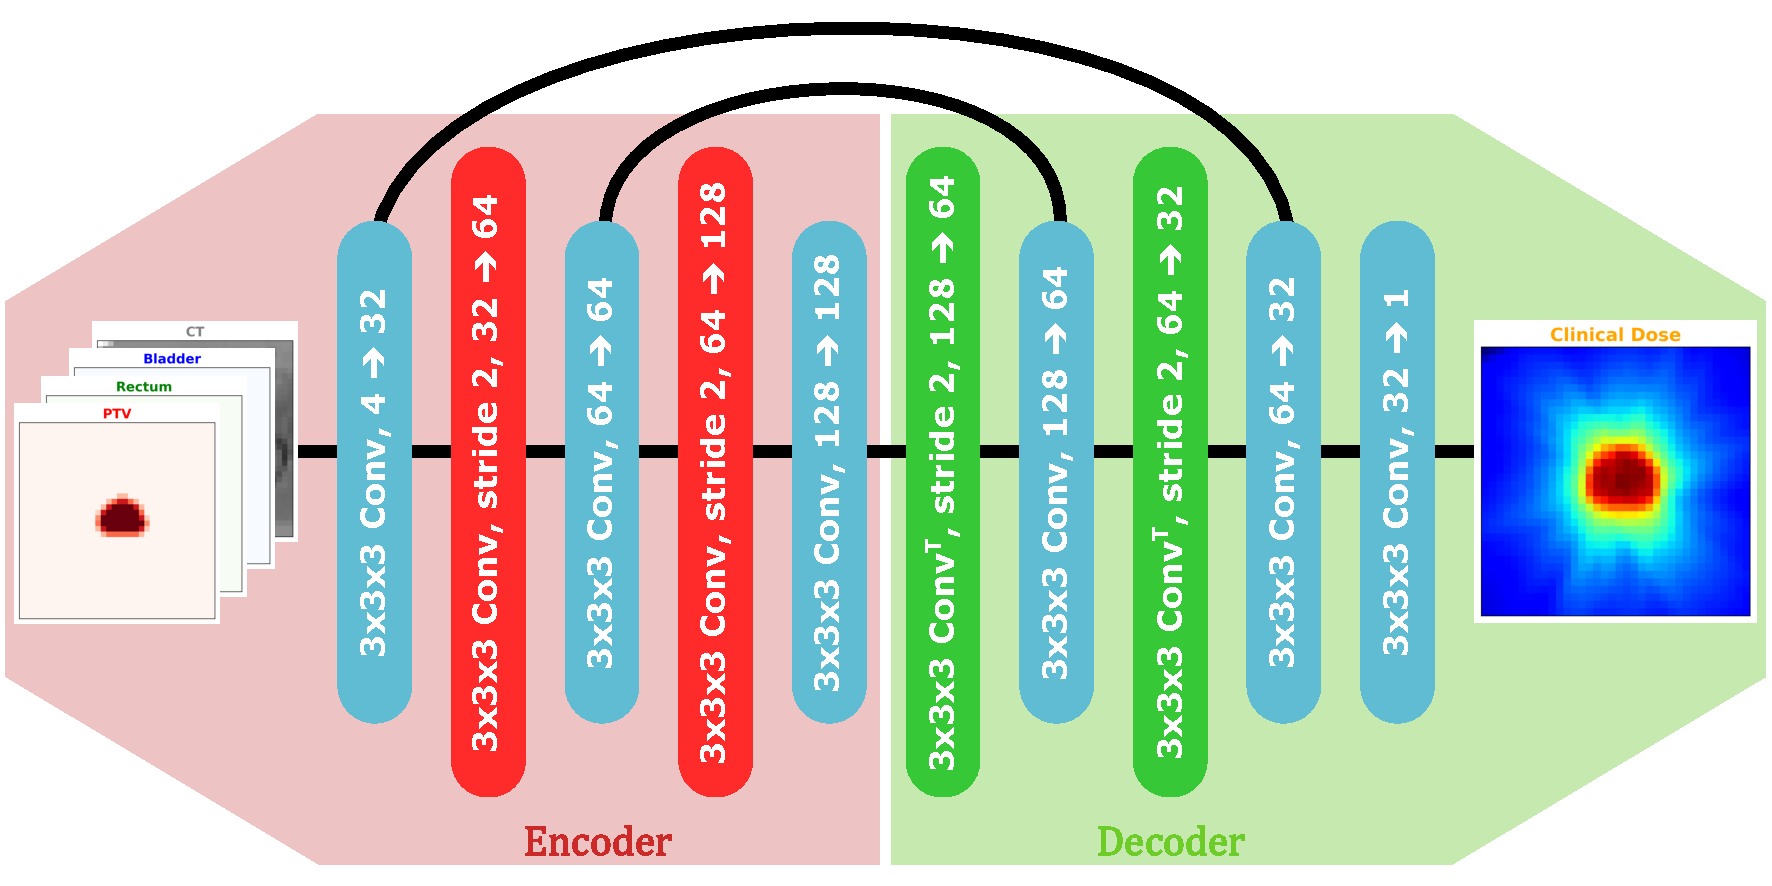
\includegraphics[width=11.5cm]{SFPM/modelC.pdf}
		\caption{Model C: No DVH data, \textbf{classical} U-net.}
		\label{fig:model_C_architecture}
	\end{subfigure}
	\begin{subfigure}{\linewidth}
		\centering
		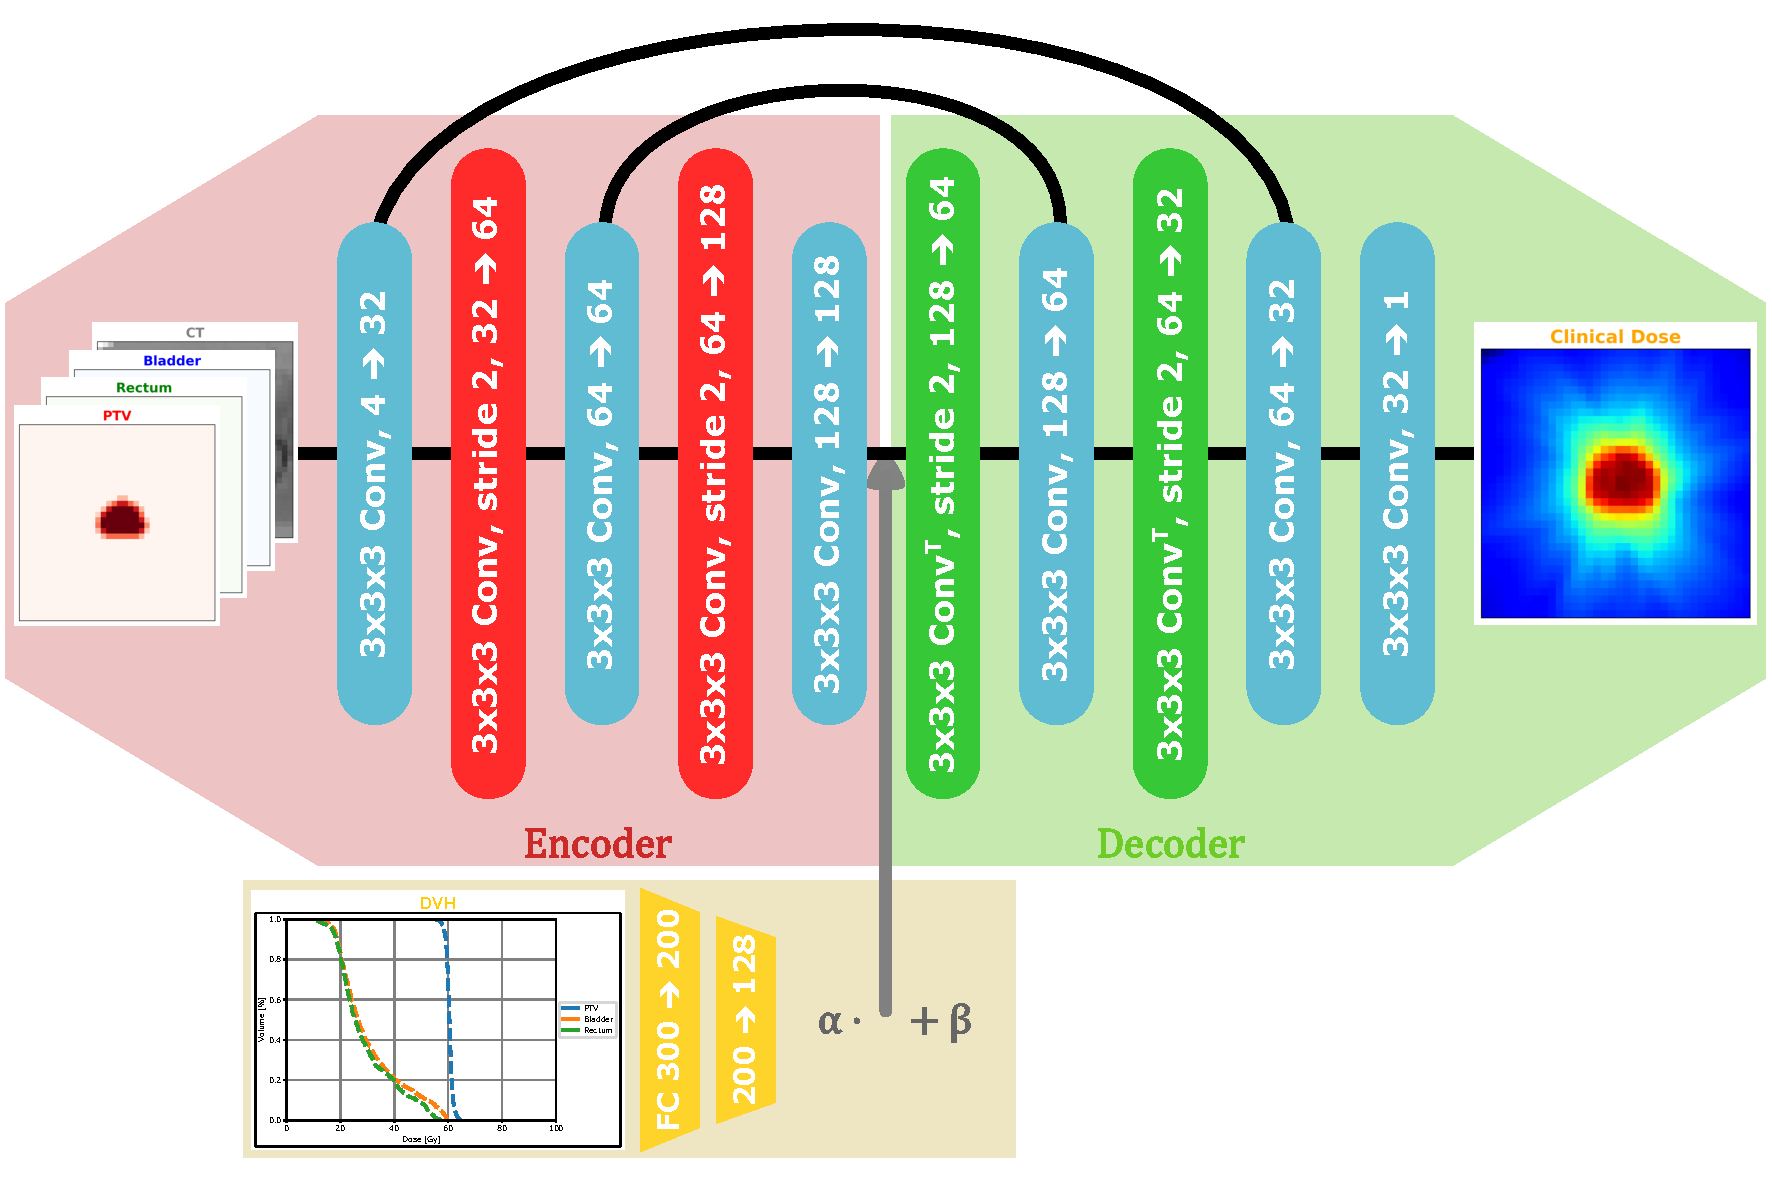
\includegraphics[width=11.5cm]{SFPM/modelB.pdf}
		\caption{Model B: DVH data using DAFT on the \textbf{bottleneck} of the U-net.}
		\label{fig:model_B_architecture}
	\end{subfigure}
	\begin{subfigure}{\linewidth}
		\centering
		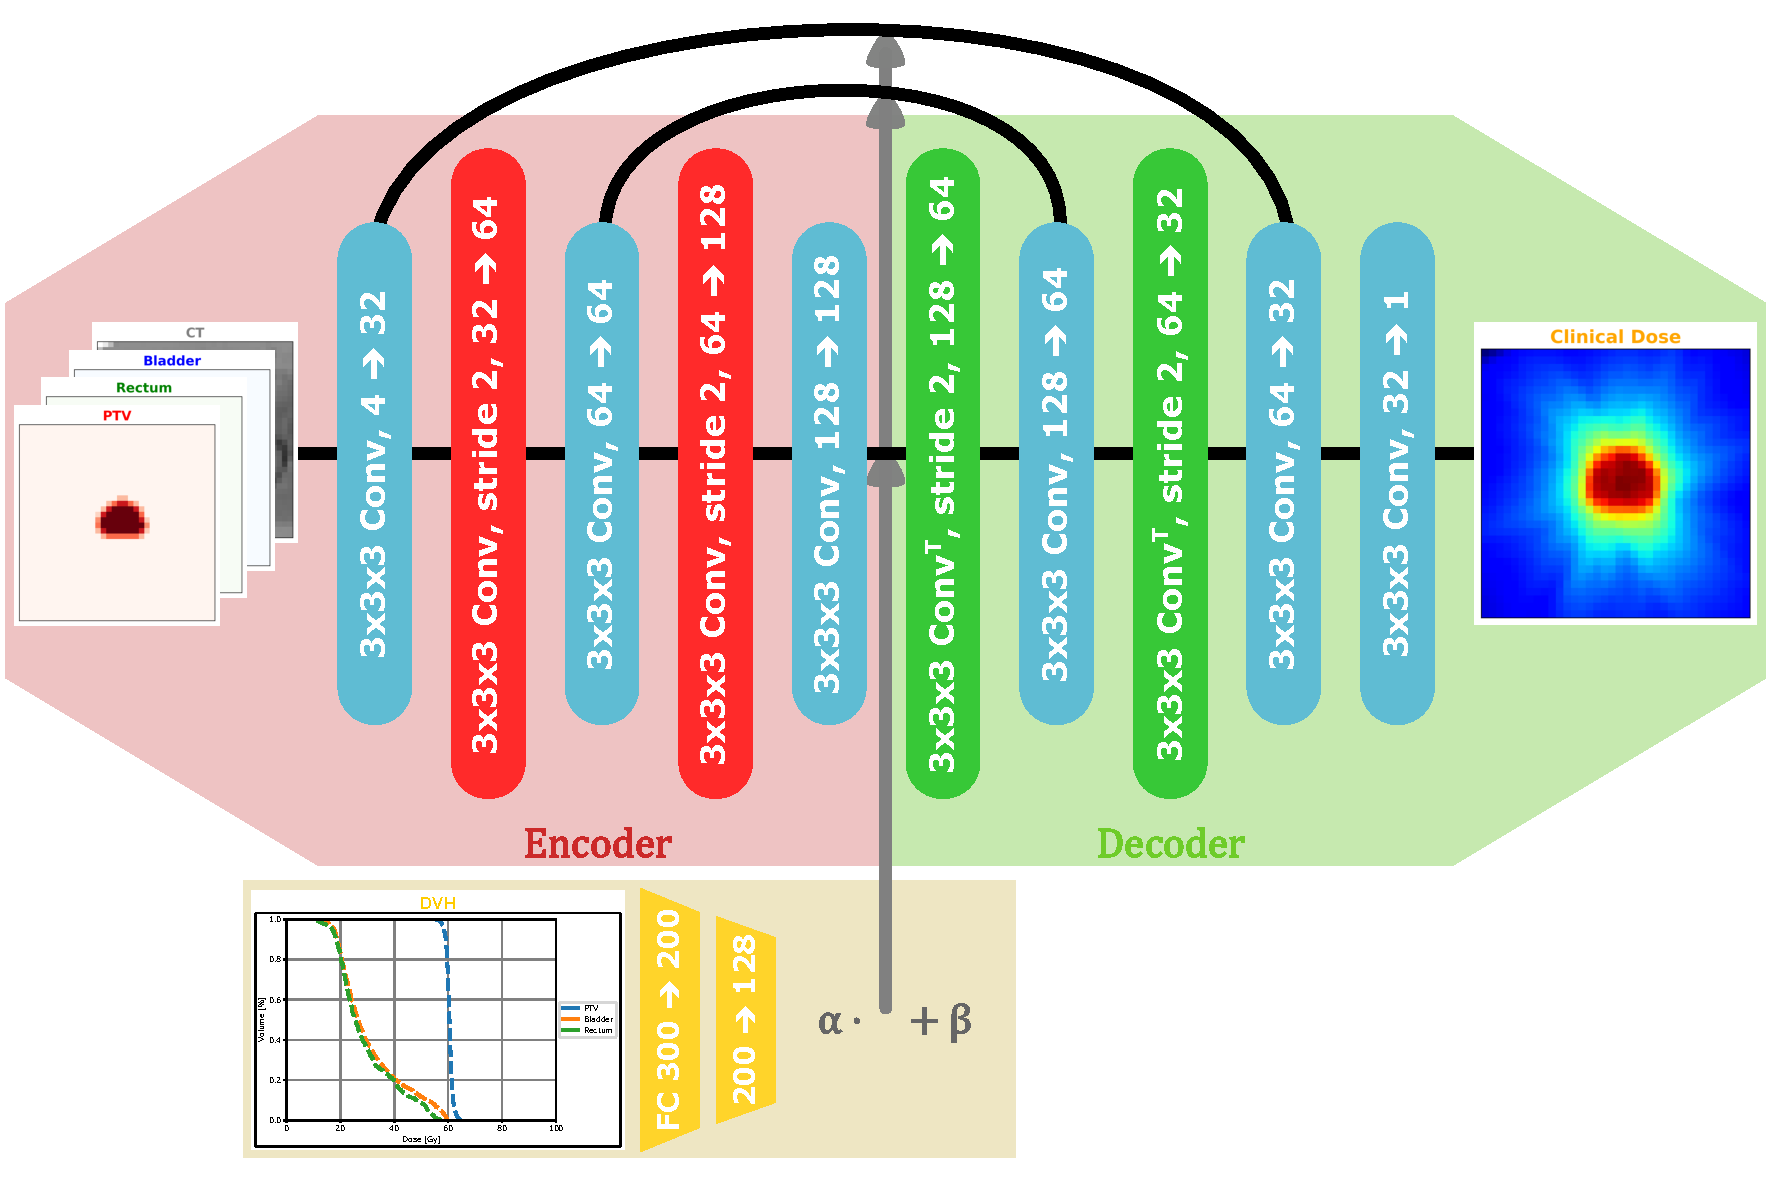
\includegraphics[width=11.5cm]{SFPM/modelA.pdf}
		\caption{Model A: DVH data using DAFT on all connections between the encoder and the decoder part of the U-net.}
		\label{fig:model_A_architecture}
	\end{subfigure}
	\caption{Architecture diagram of models A, B and C.}
	\label{fig:models_ABC_architectures}
\end{figure}

The first model referred to as "C" or the \textit{classic} model (figure \ref{fig:model_C_architecture}), consists of a standard 3D U-net architecture without any incorporation of DVH information.
The second model denoted as "B" or the \textit{bottleneck} model (figure \ref{fig:model_B_architecture}), integrates target DVH data using the DAFT technique, as described previously, at the bottleneck layer of the U-net.
In the third model, termed "A" or the \textit{all connections} model (figure \ref{fig:model_A_architecture}), DVH information is incorporated via the DAFT technique both at the bottleneck layer and across all skip connections between the encoder and decoder of the U-net.
During the model training process, the clinical DVHs corresponding to the real delivered doses were used as target DVHs for the optimization.

\subsection{Results}
Our results indicate that incorporating DVH data improves dose prediction's quantitative and qualitative aspects.

\paragraph{Quantitative Performance}
We used the Mean Absolute Error (MAE) between the predicted and ground-truth dose distributions to evaluate model performance.
The incorporation of dose-volume histogram data into the networks resulted in improved quantitative performance.
The MAE measured on the test dataset was $2.42\,\text{Gy}$ for model A, $2.58\,\text{Gy}$ for model B, and $3.18\,\text{Gy}$ for model C.

\paragraph{Prescription Adaptation}
\begin{figure}
	\centering
	\textit{(Solid line is predicted dose DVH, dotted line is target dose DVH.)}
	\begin{subfigure}{\linewidth}
		\centering
		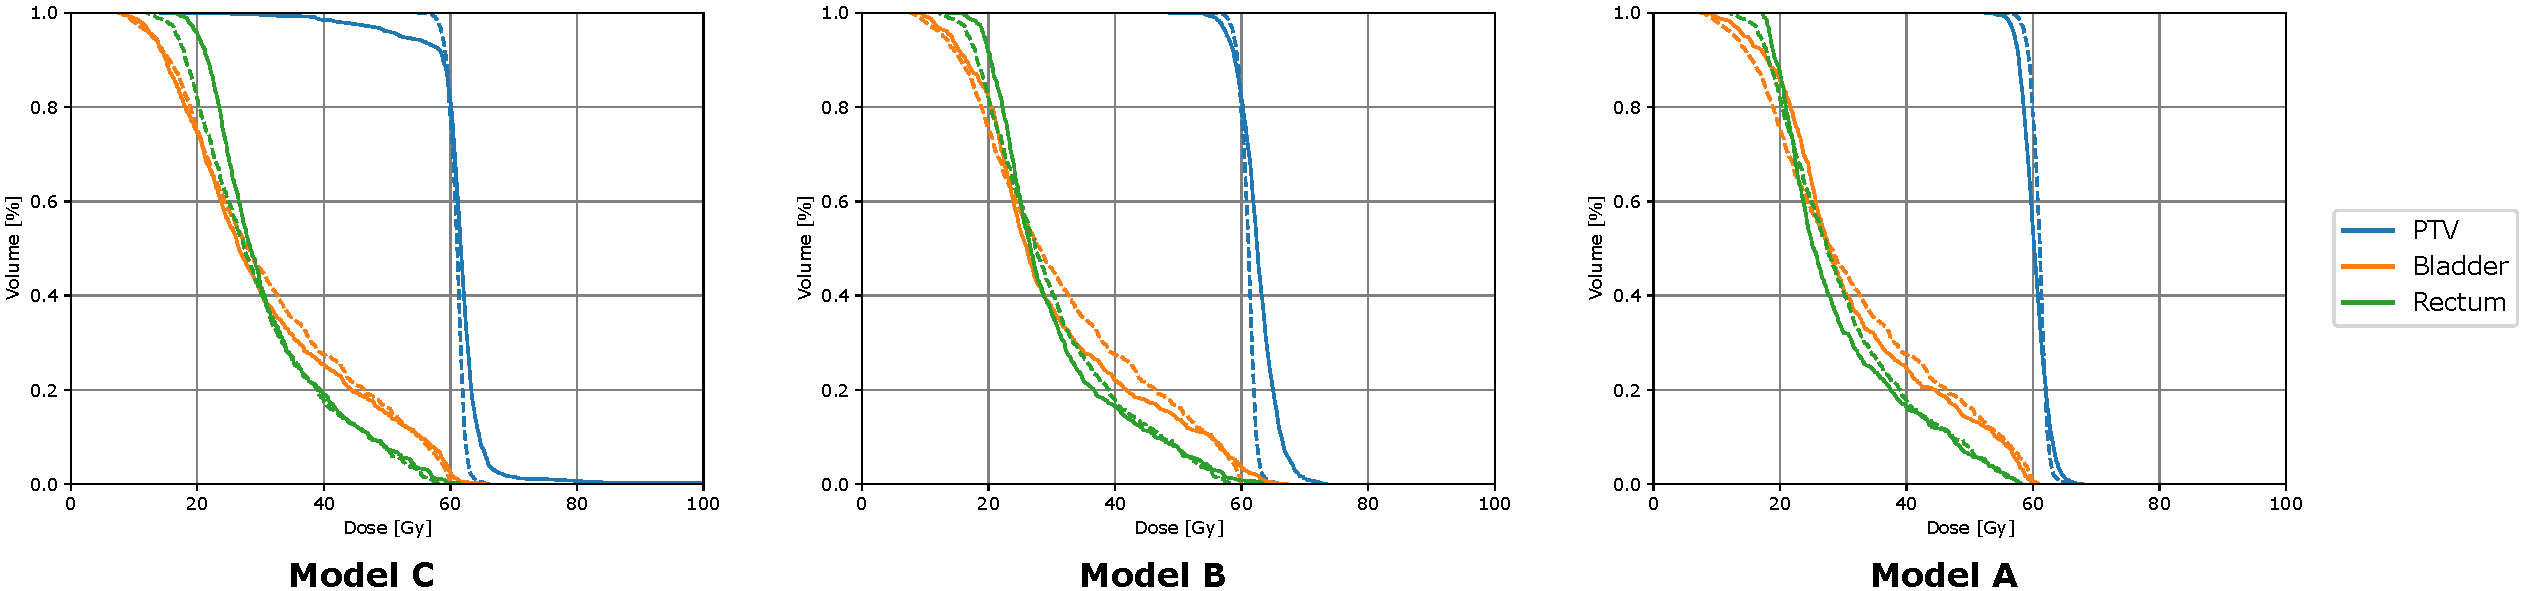
\includegraphics[width=\linewidth]{SFPM/test_patient_0.pdf}
		\caption{Patient 1, prescribed $62\,\text{Gy}$.}
		\label{fig:results_patient_1}
	\end{subfigure}
	\begin{subfigure}{\linewidth}
		\centering
		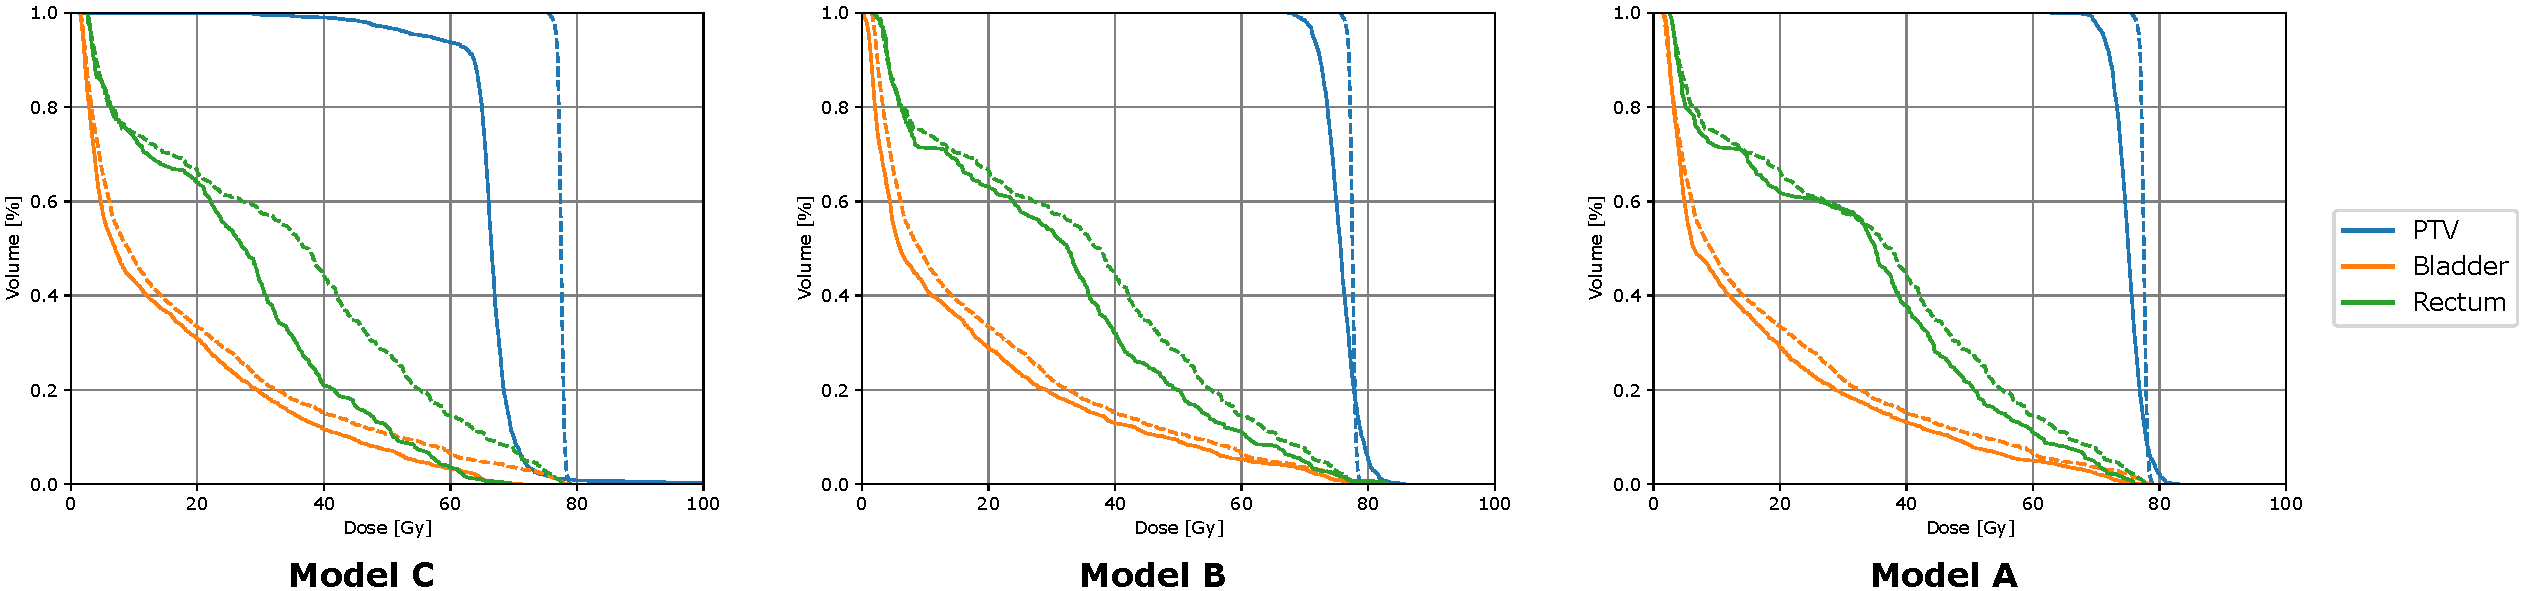
\includegraphics[width=\linewidth]{SFPM/test_patient_2.pdf}
		\caption{Patient 2, prescribed $78\,\text{Gy}$}
		\label{fig:results_patient_2}
	\end{subfigure}
	\caption{DVHs of the dose predicted by each model on two test set patients.}
	\label{fig:results_patients_12}
\end{figure}
In addition to the quantitative improvements, a qualitative analysis of the DVHs associated with the predicted dose distributions confirmed the benefit of including DVH information.
A key finding from our study was that models A and B could adapt their deep dose predictions based on the prescribed dose, with model A showing a slight advantage over model B regarding accuracy (see figure \ref{fig:results_patients_12}).
The dataset comprised patients with two distinct prescription doses: $62\,\text{Gy}$ and $78\,\text{Gy}$ to the PTV.
Model C consistently predicted dose distributions resembling a $65\,\text{Gy}$ prescription, demonstrating a lack of adaptability to the varying prescription levels (see figure \ref{fig:results_patients_12}).
In contrast, models A and B displayed greater flexibility, successfully adjusting their dose predictions following the prescribed doses for each patient.
This adaptive behavior highlights the effectiveness of incorporating DVH information, allowing the models to tailor dose predictions to specific prescription requirements.

\paragraph{Clinical Relevance}
The ability to adjust dose predictions based on DVH data demonstrates a significant advantage of our approach.
The prescription dose can vary in clinical practice depending on the tumor type, stage, and patient characteristics.
By incorporating DVH data, our models provide a more flexible and personalized approach to dose prediction, allowing the TPS to generate a plan that aligns with clinical objectives and dosimetrist input.

\subsection{Conclusions}
Our study shows the importance of incorporating DVH information into deep learning-based dose prediction models.
In this study, the target DVH links the clinical objectives defined by the dosimetrist and the predicted dose distribution.
We create a system allowing center-dependent adjustments by embedding this information into the model.
This system also allows interactive adjustment of the dose distribution when the proposed treatment plan is close to clinically acceptable.
The comparison of models A, B, and C highlights the advantages of integrating DVH data in the network.
The comparison also shows that integrating the information once at the bottleneck is sufficient.

An additional advantage of the proposed method is the capacity to generate standardized target DVH templates for treatment planning.
While averaging 3D dose distributions across multiple patients is not feasible, it is possible to compute average DVHs.
These average DVHs can be stratified by anatomical site, prescription dose, and clinical practice, providing a target for dose prediction with no effort.
Dosimetrists and doctors can further modify these templates to meet specific clinical requirements in case of non-standard patients.
Once an optimal set of DVHs is established for a given center's protocols, it can be reused for future patients with only minor adjustments.
This framework could enhance the efficiency and consistency of the treatment planning process.

Our proposed approach demonstrates the feasibility and benefits of incorporating DVH data into deep learning-based dose prediction models for radiotherapy treatment planning.
By embedding DVH information, we improve dose prediction accuracy and allow for interactive fine-tuning based on clinical objectives.
This technique opens the door to a new workflow where dosimetrists can design target DVHs, and the TPS generates the deliverable treatment plan that best matches these targets.
Further studies will explore the generalizability of our model across different cancer types and radiotherapy modalities.
Additionally, clinical validation studies will be crucial to assess the real-world impact of our proposed method on treatment outcomes and workflow efficiency.



%%%%%%%%%%%%%%%%%%%%%%%%%%%%%%%%%%%%%%%%%%%%%%%%%%%%%%%%%%%%%%%%%%%%%%%%
%                                                                      %
%   %%%%%%%%%%%%%%%%%%%%%%%%%%%%%%%%%%%%%%%%%%%%%%%%%%%%%%%%%%%%%%%%   %
%   %%%%%%%%%%%%%%%%%%%%%%%%%%%%%%%%%%%%%%%%%%%%%%%%%%%%%%%%%%%%%%%%   %
%   %%%%%%%%%%%%%%%%%%%%%%%%%%%%%%%%%%%%%%%%%%%%%%%%%%%%%%%%%%%%%%%%   %
%   %%%%%%%%%%%%%%%%%%%%%%%%%%%%%%%%%%%%%%%%%%%%%%%%%%%%%%%%%%%%%%%%   %
%                                                                      %
%%%%%%%%%%%%%%%%%%%%%%%%%%%%%%%%%%%%%%%%%%%%%%%%%%%%%%%%%%%%%%%%%%%%%%%%



% https://github.com/pauldubois98/SFRO2024
\section{Attention Mechanism on Dose-Volume Histograms for Deep Dose Predictions (SFRO 2024)}
\subsection{Introduction}
This study builds on work from the previous section
We explore using attention mechanisms to improve the incorporation of target Dose-Volume Histogram information into deep-learning models for radiotherapy dose prediction.
In traditional radiotherapy planning, DVHs are essential for assessing and optimizing dose distributions for the Principal Target Volume and Organs at Risk.
However, existing deep learning models for dose prediction, while capable of generating accurate 3D dose distributions, often fail to integrate DVH constraints fully.
This limitation reduces their utility in real-time treatment planning.

In previous work, deep learning approaches primarily focused on predicting dose distributions directly from patient imaging data, such as CT scans and anatomical contours of the PTV and OARs.
These methods typically rely on convolutional neural networks (CNNs), like the Unet, trained with voxel-wise loss functions \cite{Ronneberger2015}.
While successful in producing accurate 3D dose maps, they generally treat DVH-related information as secondary, with little attention given to adapting predictions based on these critical clinical metrics.

In the last section, we proposed integrating target DVH into the deep dose model to address this gap.
In this section, we extend prior approaches by proposing attention mechanisms to integrate target DVH information more effectively into the dose prediction process.
Attention mechanisms, widely adopted in domains such as natural language processing and image recognition, enable models to focus on relevant features within the input data selectively.
By leveraging attention, we aim to enhance the model's capacity to dynamically adapt its dose predictions following specified DVH constraints, providing a more precise and clinically responsive framework for radiotherapy treatment planning.

This work evaluates three Unet-based architectures, including a novel model using a cross-attention mechanism to incorporate DVH information into the dose prediction process directly.
Our goal is to enhance the accuracy and adaptability of deep learning models for dose prediction, ultimately enabling dosimetrists to have greater control over the treatment planning process through DVH-guided model interactions.

\subsection{Material and Methods}
\paragraph{Patient Data and Preprocessing}
We again used the cohort of 168 patients from the previous section who had undergone radiotherapy treatment.
The dataset included patients prescribed 62 Gy or 78 Gy on the PTV.
The dataset was randomly split into 80\% for training, 10\% for validation, and 10\% for testing.
We collected the CT scans, PTV contours, and OAR contours for each patient.
The CT data was resampled to a voxel size of $0.5 \times 0.5 \times 0.5 \textit{mm}^3$ to standardize inputs across patients.
As in the last section, we used the same box $120 \times 180 \times 180\ \text{mm}^3$ centered on the PTV.

\paragraph{Model Architecture and Training}
The backbone architecture for all models in this study is a 3D-convolutional Unet, a commonly used CNN for image-to-image translation tasks, such as segmentation and dose prediction.
Our U-net is of depth two, meaning it performs two levels of down-sampling and up-sampling.
The U-net outputs a 3D dose prediction for each voxel within the patient's anatomy.
Details architecture diagrams can be found in figure \ref{fig:unets012}.

\subparagraph{U-net 0 (Baseline)}
The first model, U-net 0 (architecture diagram can be found on figure \ref{fig:unet0}), serves as a baseline and does not incorporate target DVH information.
It receives the CT scan, PTV, and OAR contours as input and predicts the 3D dose distribution purely from this spatial data.

\subparagraph{U-net 1 (DVH with DAFT)}
The second model, U-net 1 (architecture diagram can be found on figure \ref{fig:unet1}), incorporates DVH data using the DAFT approach, like in the previous section.
In this model, the target DVHs are provided as additional inputs, and the model is trained to predict 3D dose distributions that match these target DVHs.

\subparagraph{U-net 2 (DVH with Cross-Attention)}
Our novel contribution, U-net 2 (architecture diagram can be found on figure \ref{fig:unet2}), integrates DVH data using a cross-attention mechanism.
In this architecture, the model takes queries from the 3D dose prediction and keys and values from the target DVHs.
The result of the 4-head attention mechanism is the same shape as that of the 3D input.
The cross-attention mechanism allows the model to adjust its dose predictions dynamically based on the desired DVH information.
The output of the attention mechanism is re-injected into the U-net during the decoding process, modifying the predicted dose map to match the target DVHs better.

\begin{figure}
	\centering
	\vspace{-0.5cm}
	\begin{subfigure}{\linewidth}
		\centering
		\includegraphics[width=12cm]{SFRO/model0.pdf}
		\caption{U-net 0: no DVH information.}
		\label{fig:unet0}
	\end{subfigure}
	\vspace{0.5cm}
	
	\begin{subfigure}{\linewidth}
		\centering
		\includegraphics[width=12cm]{SFRO/model1.pdf}
		\caption{U-net 1: DVH with DAFT.}
		\label{fig:unet1}
	\end{subfigure}
	\vspace{0.5cm}
	
	\begin{subfigure}{\linewidth}
		\centering
		\includegraphics[width=12cm]{SFRO/model2.pdf}
		\caption{U-net 2: DVHs with cross-attention.}
		\label{fig:unet2}
	\end{subfigure}
	\caption{Architecture diagrams of U-nets 0, 1 and 2.}
	\label{fig:unets012}
\end{figure}

\paragraph{Loss Function and Optimization}
The models were trained using a loss function that combines voxel-wise Mean Absolute Error (MAE) with an L1 loss on the Dose-Volume Histogram (DVH), designed to penalize deviations between the predicted and target DVHs.
Incorporating the L1 loss on DVH significantly improved the model’s convergence.
The total loss function is expressed as:
$$
\text{Total Loss} = \alpha \cdot \text{MAE}_{\text{voxel}} + \beta \cdot \text{L1}_{\text{DVH}}
$$
where $\alpha$ and $\beta$ are hyper-parameters that control the relative contribution of the two terms.
For this study, we set both $\alpha$ and $\beta$ to $1$, based on performance observed on the validation set.
However, future work could further optimize these parameters to enhance model performance.

The models were trained using the Adam optimizer with a $10^{-4}$ learning rate.
Using the validation loss criterion, early stopping was applied to prevent overfitting and ensure robust generalization.

\subsection{Results}
\paragraph{Evaluation Metrics}  
The performance of the models was assessed using two primary metrics.
The first metric was the 3D Dose Mean Absolute Error (MAE), which measures the voxel-wise MAE between the predicted dose distributions and the corresponding ground truth values.
The second metric was the Dose-Volume Histogram (DVH) deviation, calculated as the mean L1 deviation between the predicted and target DVHs for both the Principal Target Volume (PTV) and Organs at Risk (OARs).
These metrics provide a comprehensive evaluation of the models' accuracy in predicting dose distributions and adherence to clinical DVH constraints.

\paragraph{Models Performances}
The performance of the three models is summarized in Table \ref{tab:model_performance}.
Both U-net 1 and U-net 2, which incorporated DVH information, outperformed the baseline U-net 0 across all metrics.

\begin{table}
	\centering
	\begin{tabular}{|l|c|c|c|}
		\hline
		\textbf{Metric}         & \textbf{Unet-0} & \textbf{Unet-1} & \textbf{Unet-2} \\
		\hline
		3D Dose MAE (Gy)        & 3.093           & 2.254           & 2.210           \\
		\hline
		Mean DVH Deviation (Gy) & 1.942           & 1.051           & 0.930           \\
		\hline
	\end{tabular}
	\caption{Models performances comparison.}
	\label{tab:model_performance}
\end{table}

As shown, the inclusion of DVH data significantly reduced the MAE in the predicted dose distributions.
Unet-2, which used a cross-attention mechanism, showed the best overall performance, with a minor error reduction compared to U-net 1.

\paragraph{Prescription Adaptability}
The ability of the models to adapt to varying prescriptions was also evaluated.
Similarly to the last section, U-net 0 struggled to predict the correct dose when the prescription varied from its training distribution.
Regardless of the actual prescription, the model consistently predicted doses around $65\,\textit{Gy}$.
In contrast, U-net 1 and U-net 2 adapted their dose predictions to the provided DVHs, making them more versatile in clinical scenarios where the prescription may differ across patients.
There were only a few differences between the performances of U-net 1 and U-net 2.

\subsection{Conclusions}
This study re-demonstrates the feasibility of incorporating DVH data into deep-learning models for radiotherapy dose prediction.
We have marginally improved model performances and adaptability by using an attention mechanism to integrate target DVHs.
The cross-attention mechanism, in particular, offers a novel way to align predicted dose distributions with clinical goals flexibly.

Our findings indicate that this approach could facilitate the development of a more efficient radiotherapy treatment planning workflow.
In this proposed framework, dosimetrists would focus primarily on creating standardized target DVH templates rather than manually adjusting dose distributions for each patient.
These templates would serve as a foundation, requiring minimal adjustments to accommodate individual patient-specific characteristics, thereby streamlining the treatment planning process.

Designing a template for 3D dose distributions is not feasible, as 3D doses are highly patient-specific and cannot be transferred between patients.
In contrast, DVHs are more generalizable and can be applied across different patients.
This generalizability makes them suitable for the proposed workflow, where template DVHs can be established and used with deep learning-based dose prediction models guided by target DVH.
This workflow could reduce planning time and improve consistency across patients.
Future work will explore incorporating more complex DVH structures and refining the attention mechanism to enhance model interpretability and clinical usability.

%
%[1] Ronneberger, O., Fischer, P., & Brox, T. (2015). U-net: Convolutional networks for biomedical image segmentation. In *Medical Image Computing and Computer-Assisted Intervention* (pp. 234-241). Springer.
%
%[2] Chen, J., Lu, Y., & Wang, Y. (2021). Attention mechanisms in deep learning: A review. *Neurocomputing*, 461, 483-497.
%
%[3] Mahmood, R., Babier, A., McNiven, A., & Chan, M. (2020). Dose mimicking in radiotherapy planning using deep learning. *Physics in Medicine & Biology*, 65(17), 175014.
	
	\chapter{Conclusion}
	\section{Main findings}
This manuscript has explored critical advancements in radiotherapy, particularly in dose optimization.
Dosimetry remains a crucial step in RT as it directly determines the treatment plan delivered to patients.
Dosimetry optimization ensures the delivery of the prescribed radiation dose to cancerous tissues while sparing healthy structures.
However, it is also the stage where the efficacy and safety of the treatment are defined.
Thus, improvements in this step have profound clinical importance.

Through this dissertation, we have investigated various optimization techniques.
First, we focused on constructing loss functions and comparing optimization algorithms.
We have further proposed multiple avenues for automating the dosimetry process to enhance treatment efficiency and reduce manual workloads.

\paragraph{Partially Automated Clustering-based Framework}
The partially automated clustering-based framework proposes a partially automated system for dosimetry, where human intervention remains integral to the process.
The model automates most of the dose calculation but leaves room for manual adjustments by clinicians and dosimetrists.
This half-automated approach allows dosimetrists to refine or modify the treatment plan based on their expertise, maintaining the traditional workflow while benefiting from automation to save time and improve efficiency.
The clustering strategy facilitated a more profound comprehension of the interrelationships between doses.

\paragraph{Fully Automated Reinforcement Learning with Classical Optimization Approach}
The fully automated reinforcement learning combined with the classical optimization approach takes the automation further.
Within this paradigm, dosimetrists are entirely superseded, obviating the need for their input.
The system calculates and generates the optimal treatment plan based on predefined clinical constraints and objectives without requiring post-calculation adjustments by the dosimetrist.
Our innovative approach is distinguished by its direct learning from historical dose distributions.
This system eliminates the reliance on ill-defined metrics that often fail to represent the clinical acceptability of treatment plans accurately.
We have empirically demonstrated the adaptability of this framework to diverse clinical settings, only requiring retraining to work with new institutions.
This paradigm entirely obviates the need for dosimetrist intervention, streamlining the treatment planning process.

\paragraph{Fully Automated Deep Dose Based Scheme}
It is also essential to recognize that automating the dosimetry process does not mean replicating every step a human would take.
Instead, a more strategic approach involves re-engineering the workflow to optimize its suitability for machine learning or artificial intelligence models.
Automation can streamline workflows by eliminating unnecessary complexity and standardizing treatment protocols, thus making them more efficient and reliable.

The fully automated target-DVH-guided deep dose scheme approaches offer a more balanced solution by integrating deep learning models into the fully automated dosimetry process.
These systems generate dose distributions and include the flexibility for post-calculation manual adjustments via the modification of target DVHs.
The deep learning models are trained on large datasets of treatment plans and dose distributions, learning the relationships between anatomical structures, dose distribution, and dose-volume histograms.
This knowledge enables the models to make accurate dose predictions while still allowing clinically adapted dose predictions via modification of the target DVH.
Moreover, a single model is needed, and the DVH prompt can be adapted for each center instead of creating a new model from scratch, as in the fully automated scheme.

One of the key advantages of these frameworks is that they offer both full automation and clinician control.
Dosimetrists can adjust the automated dose plan when needed, providing oversight absent from the previous approaches.
We anticipate that clinicians will make frequent adjustments during the early stages of adoption.
Later, the need for manual intervention should gradually decrease, as confidence in the deep learning models grows, and dosimetrists get better prompt the model with target DVH.
Over time, clinicians may find the model's initial dose recommendations sufficiently accurate, requiring manual optimization only in exceptional cases, significantly different to the training data.

This gradual adoption mirrors the process observed with auto-contouring systems in radiotherapy.
Initially, clinicians made numerous adjustments to the auto-generated contours, but as the technology matured, they began accepting the contours with fewer and fewer modifications.
We expect a similar trajectory with automated dosimetry systems, leading to higher acceptance in the clinical community.

\section{Limitations}
\paragraph{Partially Automated Clustering-based Framework}
The partially automated clustering-based framework, while innovative, comes with a significant hurdle:
It would require a change in the current clinical workflow.
Clinicians and dosimetrists have well-established practices; altering these routines may face resistance.
Even with partial automation, shifting habits could be difficult, as it demands additional time and training.
Since radiotherapy professionals often rely on established methods they trust, adopting this hybrid model on a broad scale might be unlikely.

\paragraph{Fully Automated Reinforcement Learning with Classical Optimization Approach}
While this full automation represents a significant leap in efficiency, it also presents challenges.
The system's rigidity can become a source of frustration for clinicians, as it does not allow for minor manual adjustments to the dose distribution, which are often necessary in practice.
When clinicians encounter situations where the automated plan requires slight modifications, they must start the entire process from scratch.
This lack of flexibility could lead to dissatisfaction and reluctance to adopt the framework, as dosimetrists may value the ability to fine-tune treatment plans.
Therefore, this approach may face significant resistance in clinical practice despite its theoretical appeal.

\paragraph{Fully Automated Deep Dose Based Scheme}
The fully automated deep dose-based scheme represents a more ambitious approach, aiming at enabling full automation and human fine-tuned plan creation.
The clinical implementation and acceptance of the target DVH framework by healthcare professionals remain to be established.
Further evaluation and validation in real-world settings are necessary to ensure its effectiveness and integration into routine clinical practice.

\paragraph{From Research to Product}
While our research has introduced several promising methodologies, there are inherent limitations.
One key challenge is transitioning from prof of concept models to real-world clinical applications.
Models developed in this research, particularly those based on deep learning, are designed with a research-oriented focus and are relatively small in scale.
To realize the full potential of the target DVH deep dose frameworks, there is a clear need to transition from the current research-oriented models to high-resolution, clinically viable products.
This transformation will require collaboration between researchers, software developers, and clinical practitioners to ensure the models are scalable, robust, and compatible with existing clinical infrastructures.

\paragraph{Future work}
The target dose-volume histogram represents the most promising avenue.
Prioritizing the development and refinement of target DVH-based approaches is our recommendation for future research.

\begin{figure}
	% \centering
	\includegraphics[width=\linewidth]{frameworks.pdf}
	\textit{
		\textbf{BOO:} Beam Orientation Optimization\\
		\textbf{FMO:} Fluence maps Optimization\\
		\textbf{LS:} Leaf Sequencing
	}
	\caption{Comparison of classical versus deep dose frameworks for the creation of treatment plans.}
	\label{fig:frameworks_comparison}
\end{figure}

\section{Long-Term Impact on Radiotherapy}
\paragraph{Treatments Standardization}
The widespread adoption of automated dosimetry will benefit patients and clinicians in the long term.
By standardizing treatment planning across centers, these systems will ensure that all patients, regardless of location, have access to high-quality treatments based on the best clinical practices.
This standardization is particularly important for isolated clinics or those with limited specialist availability, where clinicians may lack experience dealing with rare or complex cases.
Ultimately, this standardization will lead to more equitable access to advanced radiotherapy treatments, improving patient outcomes on a global scale.

\paragraph{Conclusion}
The research presented in this thesis has demonstrated the importance and feasibility of automating the dosimetry process in radiotherapy.
While there are challenges in clinical adoption and model scalability, the future of radiotherapy will undoubtedly move toward more automated systems.
Among the various frameworks explored, the deep dose approach provides the most promising pathway for effective automation, offering a blend of full automation and manual adjustment flexibility.
This balance will likely encourage gradual adoption, leading to a new era in radiotherapy where treatment planning is faster, more precise, and universally accessible.

	\chapter{Perspectives}
	
	\bibliographystyle{alpha}
	\bibliography{
		1_background/1_ref.bib,
		3_dosimetry_optimization/3_ref.bib,
		3_dosimetry_optimization/optimizers_comparison.bib,
		4_doses_relations/dose_distances_refs.bib,
		4_doses_relations/dose_clustering_refs.bib,
	}
	

\end{document}
